% IDSS project report, LaTeX version (Step 14), in the format of the Word report (college format).
% Generated by scripts/build_latex.py from docs/report/*.md: edit the Markdown sources and re-run the script.
% Compile with pdfLaTeX: latexmk -pdf main.tex   (Overleaf: Menu > Compiler > pdfLaTeX)
\documentclass[12pt,a4paper,oneside]{report}

% ---- page layout
\usepackage[a4paper,top=1in,bottom=1.15in,left=1.5in,right=0.6in,footskip=0.7in]{geometry}

% ---- fonts: Times (newtx) for text and maths, EB Garamond for captions, Inconsolata for code
\usepackage[T1]{fontenc}
\usepackage[utf8]{inputenc}
\usepackage{newtxtext}
\usepackage[lining]{ebgaramond}  % after newtxtext (both define \sufigures); only used for captions
\renewcommand*{\rmdefault}{ntxtlf}  % ebgaramond switches the roman family: Times stays the body font
\usepackage{newtxmath}
\usepackage[varqu,scaled=0.95]{zi4}
\usepackage{pifont}  % \ding{51} check mark, \ding{55} cross
\IfFileExists{tfrupee.sty}{\usepackage{tfrupee}}{}
\providecommand{\rupee}{Rs.\,}  % fallback if the tfrupee font is not installed
\usepackage{microtype}

% ---- spacing: 1.5 lines, justified, 1 cm first-line indent (none after a heading)
\usepackage{setspace}
\onehalfspacing
\setlength{\parindent}{1cm}
\setlength{\emergencystretch}{2em}

% ---- headings
\usepackage{titlesec}
\titleformat{\chapter}[display]
  {\normalfont\bfseries\fontsize{16}{19}\selectfont\filleft}
  {\chaptertitlename\ \thechapter}{6pt}{}
  [{\vspace{4pt}\titlerule[2.25pt]\vspace{6pt}}]
\titleformat{name=\chapter,numberless}[block]
  {\normalfont\bfseries\fontsize{20}{24}\selectfont\filcenter}{}{0pt}{}
\titlespacing*{\chapter}{0pt}{0pt}{18pt}
\titleformat{\section}{\normalfont\bfseries\fontsize{18}{22}\selectfont}{\thesection}{0.5em}{}
\titlespacing*{\section}{0pt}{12pt plus 2pt minus 1pt}{6pt}
\titleformat{\subsection}{\normalfont\bfseries\fontsize{14}{17}\selectfont}{\thesubsection}{0.5em}{}
\titlespacing*{\subsection}{0pt}{12pt plus 2pt minus 1pt}{6pt}
\setcounter{secnumdepth}{2}
\setcounter{tocdepth}{1}

% ---- lists
\usepackage{enumitem}
\setlist{itemsep=0pt,parsep=0pt,topsep=4pt,partopsep=0pt}

% ---- colours, tables, figures
\usepackage[table]{xcolor}
\definecolor{tableheader}{HTML}{D9D9D9}
\definecolor{codebg}{HTML}{F2F2F2}
\definecolor{codeframe}{HTML}{808080}
\usepackage{array}
\usepackage{longtable}
\setlength{\LTcapwidth}{\linewidth}
\usepackage{graphicx}
\usepackage{float}
\usepackage{placeins}  % \FloatBarrier before every section keeps figures in their section
\renewcommand{\topfraction}{0.9}
\renewcommand{\bottomfraction}{0.8}
\renewcommand{\textfraction}{0.07}
\renewcommand{\floatpagefraction}{0.75}
\setcounter{topnumber}{3}
\setcounter{totalnumber}{4}

% ---- captions: EB Garamond bold 12 pt, centred, "Figure 4.1:"; figures below, tables above
\usepackage{caption}
\DeclareCaptionFont{idsscaption}{\ebgaramond}
\captionsetup{font={idsscaption,bf,normalsize,stretch=1},labelsep=colon,justification=centering,skip=6pt}
\captionsetup[figure]{position=bottom}
\captionsetup[table]{position=top}

% ---- code listings: Inconsolata 10 pt, single spacing, light grey box
\usepackage{listings}
\lstset{basicstyle=\linespread{1}\ttfamily\fontsize{10}{12}\selectfont, columns=fixed, basewidth=0.5em,
  keepspaces=true, showstringspaces=false, frame=single, framesep=4pt, framerule=0.4pt,
  rulecolor=\color{codeframe}, backgroundcolor=\color{codebg}, xleftmargin=4.4pt, xrightmargin=4.4pt,
  breaklines=true, escapeinside={(*@}{@*)}, aboveskip=8pt, belowskip=8pt, captionpos=t, tabsize=4}
\captionsetup[lstlisting]{position=top}
\newcommand{\code}[1]{\texttt{#1}}

% ---- footer: college name and the centred page number
\usepackage{fancyhdr}
\newcommand{\footerblock}[1]{\parbox[b]{\linewidth}{\centering\fontsize{10}{12}\selectfont
  G H Raisoni College of Engineering and Management, Jalgaon\par\vspace{2pt}{\normalsize #1}}}
\fancypagestyle{idss}{\fancyhf{}\renewcommand{\headrulewidth}{0pt}\renewcommand{\footrulewidth}{0pt}%
  \fancyfoot[C]{\footerblock{\thepage}}}
\fancypagestyle{plain}{\fancyhf{}\renewcommand{\headrulewidth}{0pt}\renewcommand{\footrulewidth}{0pt}%
  \fancyfoot[C]{\footerblock{\thepage}}}
\fancypagestyle{collegeonly}{\fancyhf{}\renewcommand{\headrulewidth}{0pt}\renewcommand{\footrulewidth}{0pt}%
  \fancyfoot[C]{\footerblock{}}}

% ---- page index and lists of figures / tables as in the Word report: "Chapter | Title | Page No."
\usepackage{etoolbox}
\makeatletter
\patchcmd{\l@chapter}{1.5em}{5em}{}{}
\renewcommand*{\l@section}{\@dottedtocline{1}{6.8em}{2.5em}}
\renewcommand*{\l@figure}{\@dottedtocline{1}{0em}{5em}}
\renewcommand*{\l@table}{\@dottedtocline{1}{0em}{5em}}
\newcommand{\indexheader}[2]{\noindent\makebox[5em][l]{\textbf{#1}}\textbf{#2}\hfill\textbf{Page No.}\par
  \vspace{6pt}}
\newcommand{\frontentry}[1]{\phantomsection\addcontentsline{toc}{chapter}{\protect\numberline{}#1}}
\newcommand{\indexbody}[1]{{\linespread{1}\selectfont\setlength{\parskip}{2pt plus 1pt}\@starttoc{#1}}}
\renewcommand{\contentsname}{Page Index}
\renewcommand{\bibname}{References}
\renewcommand{\tableofcontents}{\chapter*{\contentsname}\frontentry{\contentsname}%
  \indexheader{Chapter}{Title}\indexbody{toc}}
\renewcommand{\listoffigures}{\chapter*{\listfigurename}\frontentry{\listfigurename}%
  \indexheader{Sr. No.}{Figure Name}\indexbody{lof}}
\renewcommand{\listoftables}{\chapter*{\listtablename}\frontentry{\listtablename}%
  \indexheader{Sr. No.}{Table Name}\indexbody{lot}}
\makeatother

% ---- links (no coloured boxes in print); pseudo-code after hyperref
\usepackage[hyphens]{url}
\urlstyle{same}
\usepackage[hidelinks,bookmarksnumbered]{hyperref}
\hypersetup{pdftitle={Intelligent Decision Support System Using Generative AI and Machine Learning}, pdfauthor={Raj Vishwas Patil, Bhavesh Vinod Patil, Chaitany Rajesh Naval, Varun Darshan Patil}, pdfsubject={B.Tech CSE (Data Science) project report, G H Raisoni College of Engineering and Management, Jalgaon}}
\usepackage[chapter]{algorithm}
\floatstyle{plaintop}
\restylefloat{algorithm}
\captionsetup[algorithm]{position=top}
\usepackage{algpseudocode}

\begin{document}
% Front matter in the page sequence of the Word report. Generated by scripts/build_latex.py
% from docs/report/00_front_matter.md and the team details in scripts/report_common.py.

% ---- title page (not numbered)
\pagenumbering{Alph}
\begin{titlepage}
\centering
\linespread{1.15}\selectfont
{\fontsize{12}{14}\selectfont A\par}
{\fontsize{16}{19}\selectfont\bfseries Project Report\par}
{\fontsize{12}{14}\selectfont on\par}
\vspace{6pt}
{\fontsize{20}{24}\selectfont\bfseries INTELLIGENT DECISION SUPPORT SYSTEM USING GENERATIVE AI AND MACHINE LEARNING\par}
\vspace{12pt}
{\fontsize{12}{14}\selectfont submitted for Partial Fulfillment of\par}
{\fontsize{12}{14}\selectfont the Requirements of the Degree\par}
{\fontsize{12}{14}\selectfont of\par}
{\fontsize{16}{19}\selectfont\bfseries Bachelor of Technology\par}
{\fontsize{12}{14}\selectfont in\par}
{\fontsize{16}{19}\selectfont\bfseries CSE (Data Science)\par}
{\fontsize{12}{14}\selectfont to\par}
{\fontsize{16}{19}\selectfont\bfseries G H Raisoni College of Engineering and Management, Jalgaon\par}
\vspace{12pt}
{\fontsize{12}{14}\selectfont Submitted by\par}
\vspace{4pt}
{\fontsize{14}{17}\selectfont\bfseries Raj Vishwas Patil\par}
{\fontsize{14}{17}\selectfont\bfseries Bhavesh Vinod Patil\par}
{\fontsize{14}{17}\selectfont\bfseries Chaitany Rajesh Naval\par}
{\fontsize{14}{17}\selectfont\bfseries Varun Darshan Patil\par}
\vspace{12pt}
{\fontsize{12}{14}\selectfont Under the Guidance of\par}
\vspace{4pt}
{\fontsize{14}{17}\selectfont\bfseries Dr. Arjun Jadhaw\par}
\vfill
% College logo: put the image in figures/, uncomment the next line and delete the \vspace* below it.
% \includegraphics[height=3cm]{figures/college_logo.png}\par
\vspace*{3cm}
\vfill
{\fontsize{12}{14}\selectfont\bfseries Department of Data Science\par}
{\fontsize{14}{17}\selectfont G H Raisoni College of Engineering and Management,\par}
{\fontsize{14}{17}\selectfont Jalgaon -- 425002 (MS)\par}
{\fontsize{14}{17}\selectfont 2026--2027\par}
\end{titlepage}

% ---- certificate (page i, number not printed)
\pagestyle{idss}
\pagenumbering{roman}
\thispagestyle{collegeonly}
\begin{center}
\linespread{1}\selectfont
{\fontsize{16}{19}\selectfont\bfseries G H Raisoni College of Engineering and Management, Jalgaon\par}
\vspace{6pt}
{\fontsize{12}{14}\selectfont\bfseries Department of Data Science\par}
\vspace{30pt}
{\fontsize{20}{24}\selectfont\bfseries CERTIFICATE\par}
\end{center}
\vspace{18pt}
\noindent This is to certify that the project entitled ``\textbf{\textit{Intelligent Decision Support System Using Generative AI and Machine Learning}}'', submitted by\par
\vspace{6pt}
{\centering\linespread{1.3}\selectfont\bfseries
Raj Vishwas Patil\par
Bhavesh Vinod Patil\par
Chaitany Rajesh Naval\par
Varun Darshan Patil\par
}
\vspace{6pt}
\noindent in partial fulfillment of the degree of \textit{Bachelor of Technology} in \textit{CSE (Data Science)} has been satisfactorily carried out under my guidance as per the requirement of G H Raisoni College of Engineering and Management, Jalgaon.\par
\vspace{12pt}
\noindent\textbf{Date:} \rule{4.5cm}{0.4pt}\par
\noindent\textbf{Place:} Jalgaon\par
\vspace{60pt}
\noindent\begin{tabular}{@{}>{\centering}p{0.48\linewidth}@{\hspace{0.04\linewidth}}>{\centering\arraybackslash}p{0.48\linewidth}@{}}
\rule{5.5cm}{0.4pt} & \rule{5.5cm}{0.4pt} \\
\textbf{Dipak Patil} & \textbf{Dr. Arjun Jadhaw} \\
Head of Department & Project Guide \\
Department of Data Science & Department of Data Science \\
\end{tabular}
\clearpage

% ---- acknowledgement (page ii)
\chapter*{Acknowledgement}
\begingroup
\setlength{\parindent}{0pt}\setlength{\parskip}{12pt}
We would like to express our sincere gratitude to all those who supported and guided us throughout the successful completion of this group project titled ``Intelligent Decision Support System Using Generative AI and Machine Learning''.

First and foremost, we are deeply thankful to our project guide, Dr. Arjun Jadhaw, for the constant support, valuable feedback and encouragement we received during every stage of the project. Dr. Jadhaw's guidance greatly enhanced the quality of our work.

We are also grateful to Dipak Patil, Head of the Department of Data Science of G H Raisoni College of Engineering and Management, Jalgaon, for providing us with the necessary resources and a conducive learning environment. We thank the faculty and staff of the department for their help during the project weeks.

Finally, we would like to thank our families and friends for their constant encouragement and support. Thank you all.

\par\endgroup
\vspace{12pt}
{\renewcommand{\arraystretch}{1.3}
\noindent\hspace*{3.4in}\begin{tabular}[t]{@{}l@{}}
Raj Vishwas Patil \\
Bhavesh Vinod Patil \\
Chaitany Rajesh Naval \\
Varun Darshan Patil \\
\end{tabular}\par}

% ---- page index and the lists of figures and tables (each starts a new page)
\tableofcontents
\listoffigures
\listoftables

% ---- abbreviations and nomenclature
\chapter*{Abbreviations}
\frontentry{Abbreviations and Nomenclature}
\begingroup
\linespread{1}\selectfont\renewcommand{\arraystretch}{1.25}
\begin{longtable}{@{}p{1.5in}p{\dimexpr\linewidth-1.5in-2\tabcolsep\relax}@{}}
\textbf{Abbreviation} & \textbf{Full form} \\[2pt]
\endfirsthead
\textbf{Abbreviation} & \textbf{Full form} \\[2pt]
\endhead
AI & Artificial Intelligence \\
API & Application Programming Interface \\
ARI & Adjusted Rand Index \\
AST & Abstract Syntax Tree \\
AUC & Area Under the (ROC) Curve \\
AutoML & Automated Machine Learning \\
COCOMO & Constructive Cost Model \\
CPU & Central Processing Unit \\
CS & Comprehensive Score \\
CSV & Comma-Separated Values \\
DFD & Data Flow Diagram \\
DSS & Decision Support System \\
EM & Expectation--Maximisation \\
F1 & F1 score (harmonic mean of precision and recall) \\
FR & Functional Requirement \\
GenAI & Generative Artificial Intelligence \\
HoD & Head of Department \\
HPO & Hyperparameter Optimisation \\
HTTP & Hypertext Transfer Protocol \\
IDSS & Intelligent Decision Support System \\
JSON & JavaScript Object Notation \\
KLOC & Thousand (Kilo) Lines of Code \\
KPI & Key Performance Indicator \\
LLM & Large Language Model \\
ML & Machine Learning \\
NFR & Non-Functional Requirement \\
NPS & Normalised Performance Score \\
PDF & Portable Document Format \\
RAG & Retrieval-Augmented Generation \\
REST & Representational State Transfer \\
RI & Rand Index \\
RMSE & Root Mean Squared Error \\
RMSLE & Root Mean Squared Logarithmic Error \\
ROC & Receiver Operating Characteristic \\
SDLC & Software Development Life Cycle \\
SHAP & SHapley Additive exPlanations \\
SR & Success Rate \\
SRS & Software Requirements Specification \\
TF-IDF & Term Frequency--Inverse Document Frequency \\
TPE & Tree-structured Parzen Estimator \\
UI & User Interface \\
UML & Unified Modeling Language \\
\end{longtable}
\endgroup
\vspace{24pt}
{\centering\normalfont\bfseries\fontsize{20}{24}\selectfont Nomenclature\par}
\vspace{18pt}
\begingroup
\linespread{1}\selectfont\renewcommand{\arraystretch}{1.25}
\begin{longtable}{@{}p{1.5in}p{\dimexpr\linewidth-1.5in-2\tabcolsep\relax}@{}}
\textbf{Symbol} & \textbf{Meaning} \\[2pt]
\endfirsthead
\textbf{Symbol} & \textbf{Meaning} \\[2pt]
\endhead
\textit{t} & Decision threshold on the predicted probability of the positive class (default 0.5) \\
\textit{p} & Predicted probability of the positive class \\
\textit{\ensuremath{\varphi}}\textit{\textsubscript{j}} & SHAP value (contribution) of feature \textit{j} to one prediction \\
\textit{E} & Development effort in person-months (COCOMO) \\
\textit{D} & Development time in months (COCOMO) \\
\textit{P} & Average number of persons (\textit{E} / \textit{D}) \\
\textit{k} & Number of knowledge passages retrieved for a query \\
\textit{n} & Number of rows (records) \\
\textit{y}, \textit{\ensuremath{\hat{y}}} & True and predicted value of the target \\
\textit{g} & Train--test gap of a 0--1 metric used by the overfitting check \\
\end{longtable}
\endgroup

% ---- abstract (Arabic page numbers from here)
\clearpage
\pagenumbering{arabic}
\frontentry{Abstract}
\begin{center}
{\normalfont\bfseries\fontsize{14}{17}\selectfont ABSTRACT\par}
\end{center}
\vspace{28pt}
\noindent \textit{Many organisations hold data but lack the skills to turn it into decisions. This project presents an Intelligent Decision Support System (IDSS) that accepts a business problem in plain language together with a tabular dataset and returns a verified machine-learning model with explained, actionable decisions. Inspired by the AutoML-Agent framework, a resumable orchestrator coordinates seven LLM agents that interpret the request, plan, verify and explain, while deterministic code profiles the data, tunes scikit-learn, XGBoost and LightGBM models with Optuna, and computes SHAP explanations, what-if simulations, risk tiers and a PDF report. Every agent has an offline fallback. A FastAPI backend and a Streamlit interface make the system usable by non-experts. On five synthetic datasets with three seeds, every run completed (SR = 1.00), with NPS = 0.800 and CS = 0.900; the system beat a trivial baseline on all five datasets and passed verification in 14 of 15 runs.}\par
\vspace{12pt}
\noindent \textbf{Keywords:} Decision Support System, Generative AI, Large Language Model Agents, Automated Machine Learning, Explainable AI, SHAP, What-if Analysis\par

% Generated by scripts/build_latex.py from docs/report/ch1_introduction.md: edit the Markdown, not this file.
\chapter{Introduction}\label{ch:1}

Organisations make many decisions that depend on data: which customers to contact before they leave, how much stock to order, what price to expect for a crop, or which shipments will arrive late. The data is often already available in spreadsheets and databases; what is missing is the expertise to turn it into a reliable model, and the model into a clear recommendation. This project, the \textbf{Intelligent Decision Support System (IDSS)}, addresses that gap. A user describes a business problem in plain language and uploads a table of data; a team of Large Language Model (LLM) agents turns the request into a validated machine-learning pipeline, deterministic code trains and verifies the models, and the system returns explained, actionable decisions together with a PDF report.

\FloatBarrier
\section{Background and Motivation}\label{sec:1.1}

\subsection{Background}\label{sec:1.1.1}

\textbf{Decision support systems.} A decision support system (DSS) is a computer-based system that helps people use data, models and knowledge to solve semi-structured decision problems \cite{ref1}. Classical model-driven DSS needed an analyst to build each model by hand, and most dashboards describe what \textit{has} happened rather than predict what \textit{will} happen or suggest what to do.

\textbf{Machine learning and AutoML.} Libraries such as scikit-learn \cite{ref2}, XGBoost \cite{ref3} and LightGBM \cite{ref4} make strong predictive models available to everyone, but a trustworthy model still requires many expert decisions: the target and metric, cleaning and splitting, leakage prevention, model choice and tuning, and a fair test on unseen data. AutoML systems such as Auto-sklearn \cite{ref5} automate model selection and hyperparameter optimisation, often with the Tree-structured Parzen Estimator (TPE) \cite{ref6} as implemented in Optuna \cite{ref7}. They still expect a precisely specified problem and stop at a trained model.

\textbf{LLM agents.} Large language models can read a request in everyday language, ask clarifying questions, plan multi-step work and explain results; agent frameworks combine an LLM with tools in a loop of reasoning and acting \cite{ref8}. AutoML-Agent by Trirat, Jeong and Hwang \cite{ref9} showed that a team of specialised LLM agents can take a natural-language request all the way to a deployable model, using retrieval-augmented planning and multi-stage verification. IDSS is inspired by this work. We did not invent the idea of a multi-agent LLM framework for AutoML; our contribution is a different division of labour between the LLM and deterministic code, and a decision layer on top of the model (Section~\ref{sec:2.7}).

\subsection{Motivation}\label{sec:1.1.2}

\begin{enumerate}
  \item \textbf{The skills gap.} Small businesses, retailers and logistics teams can state their question (``Which customers are likely to leave, and what should we do?'') but rarely employ data scientists to answer it.
  \item \textbf{Accuracy is not a decision.} A good F1 score does not tell a manager what to do. Decision makers need the key drivers, the effect of possible actions, a list of whom to act on first and an honest statement of how far to trust the result. Explanation methods such as SHAP \cite{ref10} and counterfactual explanations \cite{ref11} provide these answers but are seldom packaged for non-experts.
  \item \textbf{LLMs are good with language and weak with numbers.} An LLM that writes its own training code can produce scripts that fail, leak test data or report numbers that were never computed --- unacceptable in a decision support tool.
\end{enumerate}

These points led to the guiding rule of IDSS: \textbf{the LLM plans and explains, deterministic code computes.} Agents interpret the request, rank models from a fixed list, review results and write the brief; profiling, training, evaluation, explanation and simulation are done by tested Python code, and every agent has a deterministic fallback, so the whole pipeline also runs without an LLM.

\FloatBarrier
\section{Problem Definition}\label{sec:1.2}

Given a tabular dataset \textit{D} (CSV, Excel, JSON or Parquet, up to 50 MB) and a business question \textit{q} in plain language, build a system that:

\begin{enumerate}
  \item decides whether \textit{q} can be answered from \textit{D} and asks short clarifying questions when information is missing;
  \item converts \textit{q} into a validated requirement --- task type, target column, metrics and constraints --- consistent with \textit{D};
  \item prepares the data, searches and tunes candidate models within a time budget and evaluates the chosen model exactly once on a held-out test split;
  \item verifies the result against the requirement and simple baselines, re-planning once if a check fails;
  \item explains the model, simulates what-if scenarios and derives risk tiers, actions or a forecast;
  \item writes a decision brief whose numbers are all grounded in computed facts, and a PDF / Markdown report; and
  \item offers all of this through a web interface with resumable runs, never sending raw rows, file paths or keys to the LLM.
\end{enumerate}

\FloatBarrier
\section{Scope and Objectives}\label{sec:1.3}

\subsection{Scope}\label{sec:1.3.1}

\textbf{In scope:} one table per analysis (\ensuremath{\leq} 50 MB); binary and multi-class classification, regression, single-series forecasting and clustering; a fixed model zoo built on scikit-learn, XGBoost and LightGBM tuned with Optuna; SHAP explanations, what-if simulation, risk tiers and counterfactual actions; an optional LLM through any OpenAI-compatible provider or a local Ollama model, and a fully offline mode; a FastAPI backend, an SQLite index and an eight-page Streamlit interface on one machine, listening on localhost only.

\textbf{Out of scope:} images, audio or free text as the main signal; joins across tables; multi-series forecasting; deep learning; multi-user accounts; deploying models as production services. Chapter~\ref{ch:8} returns to these limits.

\subsection{Objectives}\label{sec:1.3.2}

\begin{enumerate}
  \item To design a multi-agent architecture in which LLM agents interpret, plan, review and explain while deterministic engines perform every computation, with an offline fallback for each agent.
  \item To turn a plain-language question into a structured requirement, repaired against the data, with clarifying questions when information is missing.
  \item To build an AutoML engine that searches a fixed model zoo within budgets and constraints, tunes the decision threshold for binary classification and reads the test split exactly once.
  \item To verify every model with rule-based checks and re-plan once when a check fails.
  \item To provide decision support: key drivers, what-if simulation, risk tiers, counterfactual actions, forecasts, a grounded decision brief and a PDF report.
  \item To make the system usable by non-experts through a REST API and a web interface with resumable runs.
  \item To keep data private and the system safe: aggregates only to the LLM, keys only in \code{.env}, LLM-written code only in a sandbox, bounded loops and retries.
  \item To evaluate the system honestly with the SR, NPS and CS scores of AutoML-Agent \cite{ref9}, an ablation and a robustness study, and to test it with an automated test suite.
\end{enumerate}

\FloatBarrier
\section{Selection of Life Cycle Model for Development}\label{sec:1.4}

Table~\ref{tab:1.1} compares four software development life cycle (SDLC) models against the needs of the project.

\begin{table}[H]
\centering
\linespread{1}\small
\setlength{\tabcolsep}{4pt}
\caption{Comparison of life cycle models for IDSS}\label{tab:1.1}
\begin{tabular}{|>{\raggedright\arraybackslash\hspace{0pt}}p{\dimexpr 0.2304\linewidth-2\tabcolsep-2\arrayrulewidth\relax}|>{\raggedright\arraybackslash\hspace{0pt}}p{\dimexpr 0.3746\linewidth-2\tabcolsep-2\arrayrulewidth\relax}|>{\raggedright\arraybackslash\hspace{0pt}}p{\dimexpr 0.3951\linewidth-2\tabcolsep-2\arrayrulewidth\relax}|}
\hline
\rowcolor{tableheader}\textbf{Model} & \textbf{Main idea} & \textbf{Fit for IDSS} \\
\hline
Waterfall & Each phase is finished before the next begins & Poor: model quality and LLM behaviour can only be judged on running code, which would come late \\ \hline
Spiral & Repeated cycles driven by risk analysis & Partial: useful risk focus, but heavy for an eight-week student project \\ \hline
Agile / Scrum & Short sprints, backlog, customer reviews & Partial: we used weekly cycles but had no external product owner or daily stand-ups \\ \hline
\textbf{Iterative and incremental} & Build the system in increments, each adding a working, tested layer & \textbf{Selected}: matches the layered architecture and gives working software every week \\ \hline
\end{tabular}
\end{table}

We selected the \textbf{iterative and incremental model with one increment per week}:

\begin{itemize}
  \item \textbf{Layered architecture.} Foundation \ensuremath{\rightarrow} data \ensuremath{\rightarrow} requirements and orchestration \ensuremath{\rightarrow} AutoML \ensuremath{\rightarrow} verification \ensuremath{\rightarrow} decision layer \ensuremath{\rightarrow} API and UI \ensuremath{\rightarrow} evaluation; each layer depends only on the layers below it.
  \item \textbf{Working software every week.} Each increment ended with a runnable result (a demo script, a benchmark, an offline end-to-end run or UI pages), automated tests and a Git commit, so integration problems surfaced in the same week.
  \item \textbf{Learning from measurements.} For example, in a single demo run (seed 42) the week-4 benchmark recorded an F1 score of 0.558 on the churn data at the default 0.5 cut-off, and the decision-threshold tuning added in week 5 raised it to 0.623 on the same split; over the three evaluation seeds churn F1 rises from 0.561 to 0.649 (Section~\ref{sec:7.6}).
  \item \textbf{Fixed duration.} Eight weeks map directly to eight increments (Table~\ref{tab:3.3}).
\end{itemize}

Each increment followed the same cycle: plan the layer, design its interfaces as Pydantic schemas, implement, test, run the full suite, demonstrate and commit.

\FloatBarrier
\section{Organization of Report}\label{sec:1.5}

Chapter~\ref{ch:2} reviews decision support systems, AutoML, LLM agents, retrieval-augmented generation and explainable AI, and identifies the research gap. Chapter~\ref{ch:3} covers feasibility, risks, scheduling, effort allocation and a COCOMO cost estimate. Chapter~\ref{ch:4} specifies the requirements and presents the architecture, data flow diagrams, UML diagrams and the database. Chapter~\ref{ch:5} gives the algorithms, the modules, code extracts and the user interface. Chapter~\ref{ch:6} describes testing, Chapter~\ref{ch:7} the results and their discussion, and Chapter~\ref{ch:8} concludes with future scope. References, publications and two appendices (a short user manual and the weekly progress) follow.

\FloatBarrier
\section{Summary}\label{sec:1.6}

This chapter introduced IDSS, which turns a plain-language business question and a data table into a verified model and explained decisions. The motivation --- a skills gap, the need for decisions rather than only accuracy, and the weakness of LLMs with numbers --- led to the rule ``the LLM plans and explains, deterministic code computes''. We defined the problem, the scope and eight objectives, and justified the iterative and incremental life cycle with one tested increment per week.

% Generated by scripts/build_latex.py from docs/report/ch2_literature_review.md: edit the Markdown, not this file.
\chapter{Literature Review}\label{ch:2}

This chapter reviews the work on which IDSS builds: the evolution of decision support systems, automated machine learning, LLM agents, retrieval-augmented generation, explainable AI and counterfactual explanations. It then describes AutoML-Agent, the framework that inspired IDSS, compares related work and identifies the research gap.

\FloatBarrier
\section{Evolution of Decision Support Systems}\label{sec:2.1}

Power defines a decision support system as an interactive computer-based system that helps decision makers use communication technologies, data, documents, knowledge and models to identify and solve problems \cite{ref1}. He groups such systems by their dominant component into \textbf{data-driven}, \textbf{model-driven}, \textbf{knowledge-driven}, \textbf{document-driven} and \textbf{communication-driven} systems \cite{ref1}. Table~\ref{tab:2.1} summarises, in broad terms, how decision support has evolved. Each stage made more data and stronger models available, but each still kept an expert in the loop to build the model, write the query or configure the dashboard.

\begingroup
\linespread{1}\small
\setlength{\tabcolsep}{4pt}
\begin{longtable}{|>{\raggedright\arraybackslash\hspace{0pt}}p{\dimexpr 0.2425\linewidth-2\tabcolsep-2\arrayrulewidth\relax}|>{\raggedright\arraybackslash\hspace{0pt}}p{\dimexpr 0.2619\linewidth-2\tabcolsep-2\arrayrulewidth\relax}|>{\raggedright\arraybackslash\hspace{0pt}}p{\dimexpr 0.2870\linewidth-2\tabcolsep-2\arrayrulewidth\relax}|>{\raggedright\arraybackslash\hspace{0pt}}p{\dimexpr 0.2086\linewidth-2\tabcolsep-2\arrayrulewidth\relax}|}
\caption{Broad stages in the evolution of decision support}\label{tab:2.1}\\
\hline
\rowcolor{tableheader}\textbf{Stage} & \textbf{Typical tools} & \textbf{What the user receives} & \textbf{Who builds the analysis} \\
\hline
\endfirsthead
\hline
\rowcolor{tableheader}\textbf{Stage} & \textbf{Typical tools} & \textbf{What the user receives} & \textbf{Who builds the analysis} \\
\endhead
Model-driven DSS & Spreadsheet, optimisation and simulation models & Answers from one hand-built model & Analyst \\ \hline
Data-driven DSS and BI & Data warehouses, OLAP, reports, dashboards & Descriptions of what has happened & BI developers \\ \hline
Knowledge-driven DSS & Rule-based expert systems & Rule-based recommendations & Knowledge engineers \\ \hline
Predictive analytics & Machine-learning models \cite{ref2}, \cite{ref3}, \cite{ref4} & Predictions with accuracy figures & Data scientists \\ \hline
Automated ML & AutoML systems \cite{ref5} & A tuned model for a specified task & Users who can specify target, metric and data \\ \hline
LLM-assisted DSS (this project) & LLM agents + deterministic AutoML + explanations & Verified model, explanations, actions and a report from a plain-language question & The system, with the user answering questions \\ \hline
\end{longtable}
\endgroup

IDSS belongs to the last stage. It is model-driven at its core --- every recommendation comes from a trained and verified model --- but it uses an LLM for the parts that used to need an expert to talk to the user: understanding the question, asking for missing information and explaining the result.

\FloatBarrier
\section{Automated Machine Learning and Hyperparameter Optimisation}\label{sec:2.2}

\textbf{Auto-sklearn} framed AutoML as combined algorithm selection and hyperparameter optimisation over scikit-learn pipelines, using Bayesian optimisation, meta-learning to warm-start the search and an ensemble of the models found \cite{ref5}. It matches or beats manual model building on many tabular datasets, but the user must still specify the features, target, task and metric in code, and the output is a model, not a decision.

\textbf{TPE} models the hyperparameter densities of good and bad trials separately and proposes the configuration that maximises their ratio; it handles conditional, mixed search spaces cheaply \cite{ref6}. \textbf{Optuna} offers a \textit{define-by-run} API, efficient samplers such as TPE and pruners that stop unpromising trials early \cite{ref7}. IDSS uses Optuna's TPE sampler with a median pruner.

The IDSS model zoo is built from \textbf{scikit-learn}, with its consistent \code{fit} / \code{predict} interface and pipelines \cite{ref2}, \textbf{XGBoost}, which made gradient tree boosting scalable through a regularised objective and sparsity-aware split finding \cite{ref3}, and \textbf{LightGBM}, which made it faster with histogram-based, leaf-wise growth, gradient-based one-side sampling and exclusive feature bundling \cite{ref4}.

\textbf{Gap:} AutoML automates the \textit{search}, not the \textit{framing} of the problem or the \textit{use} of the result.

\FloatBarrier
\section{Large Language Model Agents}\label{sec:2.3}

An LLM agent uses a language model to decide the next step, calls tools and reads their results. \textbf{ReAct} interleaves reasoning traces with actions, so the model can plan, act, observe and correct itself, which reduces hallucination compared with reasoning alone \cite{ref8}. \textbf{AutoGen} lets several conversable agents cooperate through messages, with a human in the loop and execution of the code they write \cite{ref12}. \textbf{Data Interpreter} decomposes data-science tasks into a graph of sub-tasks and writes and executes code for each step, revising the plan when execution fails \cite{ref13}.

These systems show that LLMs can drive multi-step analyses, but also the weakness that matters most for decision support: the reported numbers come from code written during the run, which may be wrong in ways a non-expert cannot detect. IDSS therefore lets agents \textit{choose and explain} but not \textit{compute}: they pick models only from a fixed, tested zoo, and the one place where LLM-written code runs (\textit{Ask Your Data}) is isolated in a sandbox.

\FloatBarrier
\section{Retrieval-Augmented Generation}\label{sec:2.4}

Retrieval-augmented generation (RAG) combines a generator with a non-parametric memory: a retriever fetches relevant passages from an indexed corpus and the generator conditions on them, which improves factual accuracy and lets knowledge be updated without retraining \cite{ref14}. IDSS uses a lightweight, offline form of RAG for \textit{planning}: ten best-practice notes written by the team are split into chunks of about 500 characters, indexed with TF-IDF and cached; the Knowledge Agent retrieves the four most relevant passages (at most two per note) and condenses them into a brief for the Model Agent. Web search is used only when a key is configured, so retrieval stays deterministic, fast and auditable.

\FloatBarrier
\section{Explainable AI}\label{sec:2.5}

\textbf{LIME} explains one prediction by fitting a simple model to the black-box model's behaviour on perturbed samples around that record \cite{ref15}. \textbf{SHAP} unifies additive feature attributions under Shapley values and is the only additive attribution with local accuracy, missingness and consistency \cite{ref10}. A SHAP value \textit{\ensuremath{\varphi}}\textit{\textsubscript{j}} is the contribution of feature \textit{j} to moving one prediction away from the average prediction; the mean absolute values give a global ranking. IDSS uses SHAP's tree explainer for tree ensembles and the linear explainer for logistic and ridge regression (permutation importance otherwise), sums the values of derived features back to the user's original columns --- \code{contract\_\allowbreak{}type} instead of \code{cat\_\allowbreak{}\_\allowbreak{}contract\_\allowbreak{}type\_\allowbreak{}Month-\allowbreak{}to-\allowbreak{}month} --- and orients binary explanations to the positive class, so a positive value always means ``raises the risk''.

\FloatBarrier
\section{Counterfactual Explanations and What-if Analysis}\label{sec:2.6}

Wachter, Mittelstadt and Russell proposed counterfactual explanations: the smallest change to the input that would change the model's decision \cite{ref11}. Unlike feature importances, counterfactuals directly suggest an action. IDSS implements the idea twice: a \textbf{what-if simulator} that changes inputs for one record or a segment and shows the prediction before and after, and a \textbf{counterfactual search} that finds at most three changes to actionable columns, using values observed in the data, that bring a high-risk record below the decision threshold. As in the literature, these statements describe the \textit{model}, not causal effects in the real world.

\FloatBarrier
\section{AutoML-Agent and What IDSS Changes}\label{sec:2.7}

\textbf{AutoML-Agent} \cite{ref9} is a multi-agent LLM framework for full-pipeline AutoML. An agent manager receives the request, a prompt agent turns it into a structured specification, retrieval-augmented planning produces candidate plans, data and model agents carry them out, an operation agent writes and runs the code, and verification is applied to the request, the execution and the implementation. The framework is evaluated with a success rate (SR), a normalised performance score (NPS) and a comprehensive score (CS = 0.5 \ensuremath{\cdot} SR + 0.5 \ensuremath{\cdot} NPS). We read the reference implementation for ideas only; no code was copied. Tables~\ref{tab:2.2} and~\ref{tab:2.3} list what we kept and what we changed.

\begingroup
\linespread{1}\small
\setlength{\tabcolsep}{4pt}
\begin{longtable}{|>{\raggedright\arraybackslash\hspace{0pt}}p{\dimexpr 0.2708\linewidth-2\tabcolsep-2\arrayrulewidth\relax}|>{\raggedright\arraybackslash\hspace{0pt}}p{\dimexpr 0.3393\linewidth-2\tabcolsep-2\arrayrulewidth\relax}|>{\raggedright\arraybackslash\hspace{0pt}}p{\dimexpr 0.3899\linewidth-2\tabcolsep-2\arrayrulewidth\relax}|}
\caption{Ideas kept from AutoML-Agent}\label{tab:2.2}\\
\hline
\rowcolor{tableheader}\textbf{Idea} & \textbf{In AutoML-Agent} & \textbf{In IDSS} \\
\hline
\endfirsthead
\hline
\rowcolor{tableheader}\textbf{Idea} & \textbf{In AutoML-Agent} & \textbf{In IDSS} \\
\endhead
Multi-agent decomposition & Manager with prompt, data, model and operation agents & Orchestrator with Requirement, Data, Knowledge, Model, Verifier, Analysis and Insight agents, each with typed (Pydantic) inputs and outputs \\ \hline
Structured requirement parsing & Prompt agent produces a JSON specification & Requirement Agent produces a \code{UserRequirement} and repairs it against the data \\ \hline
Retrieval-augmented planning & Plans informed by retrieved knowledge & Model Agent ranks candidates with a brief retrieved from best-practice notes \\ \hline
Multi-stage verification & Request, execution and implementation verified & Relevance and sufficiency checks; audited single use of the test split; seven result checks with one re-plan \\ \hline
Evaluation metrics & SR, NPS, CS & Reproduced offline; adjusted Rand index instead of Rand index for clustering (Section~\ref{sec:7.7}) \\ \hline
\end{longtable}
\endgroup

\begin{table}[H]
\centering
\linespread{1}\small
\setlength{\tabcolsep}{4pt}
\caption{Design decisions changed in IDSS}\label{tab:2.3}
\begin{tabular}{|>{\raggedright\arraybackslash\hspace{0pt}}p{\dimexpr 0.5043\linewidth-2\tabcolsep-2\arrayrulewidth\relax}|>{\raggedright\arraybackslash\hspace{0pt}}p{\dimexpr 0.4957\linewidth-2\tabcolsep-2\arrayrulewidth\relax}|}
\hline
\rowcolor{tableheader}\textbf{Change} & \textbf{Reason} \\
\hline
The LLM only ranks names from a fixed model zoo; tested code trains, tunes, selects and evaluates & Every run that starts can finish; results are reproducible; the test split provably stays untouched; works without an LLM \\ \hline
Offline RAG over ten curated notes (TF-IDF, cached); web search only with a key & No network dependency; no data leaves the machine; auditable retrieval \\ \hline
Sandbox for the only LLM-written code (\textit{Ask Your Data}) & LLM-generated code is untrusted input \\ \hline
Decision layer: drivers on original columns, what-if, risk tiers, counterfactual actions, grounded brief, PDF report & Decision makers need to know \textit{what to do}, not only how accurate a model is \\ \hline
Persistent, resumable runs with a REST API and a web UI & Non-experts use a browser; runs survive restarts and can wait for answers \\ \hline
Fast / full budgets and parsed constraints (latency, training time, explainability) & Predictable runtime on a laptop; constraints are enforced, not only mentioned \\ \hline
\end{tabular}
\end{table}

\FloatBarrier
\section{Comparison of Related Work}\label{sec:2.8}

\begingroup
\linespread{1}\small
\setlength{\tabcolsep}{4pt}
\begin{longtable}{|>{\raggedright\arraybackslash\hspace{0pt}}p{\dimexpr 0.1870\linewidth-2\tabcolsep-2\arrayrulewidth\relax}|>{\raggedright\arraybackslash\hspace{0pt}}p{\dimexpr 0.2130\linewidth-2\tabcolsep-2\arrayrulewidth\relax}|>{\raggedright\arraybackslash\hspace{0pt}}p{\dimexpr 0.2130\linewidth-2\tabcolsep-2\arrayrulewidth\relax}|>{\raggedright\arraybackslash\hspace{0pt}}p{\dimexpr 0.1739\linewidth-2\tabcolsep-2\arrayrulewidth\relax}|>{\raggedright\arraybackslash\hspace{0pt}}p{\dimexpr 0.2130\linewidth-2\tabcolsep-2\arrayrulewidth\relax}|}
\caption{Comparison of related work with IDSS}\label{tab:2.4}\\
\hline
\rowcolor{tableheader}\textbf{Work} & \textbf{Approach} & \textbf{Strengths} & \textbf{Limitations} & \textbf{How IDSS differs} \\
\hline
\endfirsthead
\hline
\rowcolor{tableheader}\textbf{Work} & \textbf{Approach} & \textbf{Strengths} & \textbf{Limitations} & \textbf{How IDSS differs} \\
\endhead
Model- and data-driven DSS \cite{ref1} & Hand-built models, reports, dashboards & Trusted, domain-specific & Each new question needs an analyst; mostly descriptive & Builds a predictive model per plain-language question \\ \hline
Auto-sklearn \cite{ref5} & Bayesian optimisation over pipelines, meta-learning, ensembles & Strong automatic search on tabular data & Problem specified in code; output is a model & Parses the question; adds verification and decisions \\ \hline
TPE / Optuna \cite{ref6}, \cite{ref7} & Model-based hyperparameter search with pruning & Efficient, flexible & A library: objective and models must be written & Used as the tuning engine of a tested model zoo \\ \hline
ReAct \cite{ref8} & Interleaved reasoning and tool use & General; grounds reasoning in tool results & No notion of splits, baselines or model quality & Fixed state machine with bounded loops; tools are tested engines \\ \hline
AutoGen \cite{ref12} & Conversing agents that run code & Flexible workflows, human in the loop & Results depend on generated code; hard to bound & Typed hand-offs, \ensuremath{\leq} 2 clarification rounds, 1 re-plan \\ \hline
Data Interpreter \cite{ref13} & Task graph with code per step & End-to-end data analyses & Numbers come from code generated during the run & Numbers only from deterministic code; LLM code sandboxed \\ \hline
AutoML-Agent \cite{ref9} & Multi-agent LLM framework, request to deployable model & Full pipeline, systematic verification & Generated training code can fail; stops at the model & Deterministic engine, offline fallbacks, decision layer, UI \\ \hline
SHAP / LIME \cite{ref10}, \cite{ref15} & Post-hoc feature attributions & Well-founded explanations & Expert libraries; engineered feature names & Built in, on original columns, in plain language \\ \hline
\end{longtable}
\endgroup

\FloatBarrier
\section{Research Gap}\label{sec:2.9}

AutoML systems automate model search but need a precisely framed problem and return only a model. LLM agents understand plain language but compute their numbers with code generated during the run. Explanation and counterfactual methods exist but are rarely combined with model building in a tool for non-experts. We found few systems that (1) accept a plain-language question and repair it against the data, (2) compute every number with deterministic, tested code and work without an LLM, (3) audit their own evaluation and say when a result is not verified, (4) turn the model into decisions with a brief whose numbers are checked against computed facts, and (5) run as a resumable web application on a single laptop. IDSS is designed to fill this gap; its contribution is the combination and the division of labour, not a new learning algorithm.

\FloatBarrier
\section{Summary}\label{sec:2.10}

This chapter traced decision support from hand-built models to AutoML and LLM agents and reviewed RAG, SHAP, LIME and counterfactual explanations. We described AutoML-Agent, listed the ideas we kept and the decisions we changed, compared related work and identified the gap that IDSS addresses: a decision support system that is conversational at the front, deterministic in its computation, self-verifying and decision-oriented.

% Generated by scripts/build_latex.py from docs/report/ch3_planning_management.md: edit the Markdown, not this file.
\chapter{Project Planning and Management}\label{ch:3}

This chapter examines whether the project was feasible and which risks threatened it, and presents the eight-week schedule, the allocation of work among the four members and an estimate of effort and cost based on the real size of the code.

\FloatBarrier
\section{Feasibility Study and Risk Analysis}\label{sec:3.1}

\subsection{Feasibility Study}\label{sec:3.1.1}

\textbf{Technical feasibility.} Every computational part rests on mature open-source libraries --- pandas, scikit-learn \cite{ref2}, XGBoost \cite{ref3}, LightGBM \cite{ref4}, Optuna \cite{ref7}, SHAP \cite{ref10}, FastAPI, Streamlit, SQLAlchemy and reportlab --- so the work was integration rather than invention. One OpenAI-compatible client reaches OpenAI, Groq, Google Gemini or a local Ollama model, and every agent has a fallback, so no provider is required. Tabular datasets of a few thousand rows train in seconds to minutes on a laptop CPU within the \textit{fast} budget (3 models \ensuremath{\times} 15 Optuna trials, at most 180 s in total); no GPU is needed.

\textbf{Economic feasibility.} All software is free and open source and the hardware is the team's own laptops. The only possible running cost is the optional LLM API, and prompts carry aggregates only, which keeps them short.

\textbf{Operational feasibility.} The users are business users who cannot program. The system therefore offers a browser interface, plain-language questions with examples, a one-click Demo Mode, stage-by-stage progress, clarifying questions instead of error messages and results explained in words. Runs are saved after every step, so a restart loses no work.

\textbf{Schedule feasibility.} The architecture splits into eight layers that each depend only on the layers below, which allowed one layer per week. Each week's scope was kept small enough to be implemented \textit{and} tested; features that did not fit were declared out of scope. Table~\ref{tab:3.1} summarises the study.

\begin{table}[H]
\centering
\linespread{1}\small
\setlength{\tabcolsep}{4pt}
\caption{Feasibility summary}\label{tab:3.1}
\begin{tabular}{|>{\raggedright\arraybackslash\hspace{0pt}}p{\dimexpr 0.1823\linewidth-2\tabcolsep-2\arrayrulewidth\relax}|>{\raggedright\arraybackslash\hspace{0pt}}p{\dimexpr 0.2392\linewidth-2\tabcolsep-2\arrayrulewidth\relax}|>{\raggedright\arraybackslash\hspace{0pt}}p{\dimexpr 0.2101\linewidth-2\tabcolsep-2\arrayrulewidth\relax}|>{\raggedright\arraybackslash\hspace{0pt}}p{\dimexpr 0.3684\linewidth-2\tabcolsep-2\arrayrulewidth\relax}|}
\hline
\rowcolor{tableheader}\textbf{Aspect} & \textbf{Question} & \textbf{Assessment} & \textbf{Basis} \\
\hline
Technical & Can the team build and run it? & Feasible & Mature libraries; provider-independent LLM client; laptop-scale workloads \\ \hline
Economic & Can it be built without a budget? & Feasible & Open-source software; own laptops; LLM optional \\ \hline
Operational & Can non-experts use it? & Feasible & Browser UI, plain language, clarifying questions, Demo Mode \\ \hline
Schedule & Does it fit eight weeks? & Feasible with strict scope & One tested layer per week; explicit out-of-scope list \\ \hline
\end{tabular}
\end{table}

\subsection{Risk Analysis}\label{sec:3.1.2}

We identified the risks below at the start of the project and reviewed them weekly. Probability (P) and impact (I) are rated Low, Medium or High; the mitigations are implemented in the final system (Table~\ref{tab:3.2}).

\begingroup
\linespread{1}\small
\setlength{\tabcolsep}{4pt}
\begin{longtable}{|>{\raggedright\arraybackslash\hspace{0pt}}p{\dimexpr 0.0733\linewidth-2\tabcolsep-2\arrayrulewidth\relax}|>{\raggedright\arraybackslash\hspace{0pt}}p{\dimexpr 0.3120\linewidth-2\tabcolsep-2\arrayrulewidth\relax}|>{\raggedright\arraybackslash\hspace{0pt}}p{\dimexpr 0.1142\linewidth-2\tabcolsep-2\arrayrulewidth\relax}|>{\raggedright\arraybackslash\hspace{0pt}}p{\dimexpr 0.1142\linewidth-2\tabcolsep-2\arrayrulewidth\relax}|>{\raggedright\arraybackslash\hspace{0pt}}p{\dimexpr 0.3864\linewidth-2\tabcolsep-2\arrayrulewidth\relax}|}
\caption{Risk analysis}\label{tab:3.2}\\
\hline
\rowcolor{tableheader}\textbf{ID} & \textbf{Risk} & \textbf{P} & \textbf{I} & \textbf{Mitigation implemented} \\
\hline
\endfirsthead
\hline
\rowcolor{tableheader}\textbf{ID} & \textbf{Risk} & \textbf{P} & \textbf{I} & \textbf{Mitigation implemented} \\
\endhead
R1 & LLM unavailable, slow or not configured & High & High & Timeout on every call (60 s default), at most 3 retries with backoff, deterministic fallback in every agent; the pipeline runs offline \\ \hline
R2 & Hallucinated numbers in the decision brief & Medium & High & Brief built from computed facts only; grounding check rejects unsupported numbers; one regeneration, then a grounded template \\ \hline
R3 & Unsafe LLM-written code & Medium & High & Code runs only in the sandbox: AST guard, isolated child process, restricted built-ins, 20 s timeout, no secrets \\ \hline
R4 & Data leakage or reuse of the test split & Medium & High & Splits fixed before training; tuning sees only train and validation; audited single test read; leakage warning at correlation \ensuremath{\geq} 0.98 \\ \hline
R5 & LLM usage limits, rate limits or cost & Medium & Medium & Aggregates only in prompts; capped retries; LLM optional; tests use a fake LLM \\ \hline
R6 & Malformed JSON from the LLM & High & Medium & Pydantic validation with the error fed back for a retry; fallback after the retry cap \\ \hline
R7 & Requirement misunderstood & Medium & High & Deterministic repair of target, task type and metrics against the data; repairs shown; clarifying questions \\ \hline
R8 & Training too slow on a laptop & Medium & Medium & Budgets with per-model and total time limits; median pruning; one training at a time \\ \hline
R9 & Over-fitting or a model no better than trivial & Medium & High & Baseline on the same test split; train--test gap check (\textless{} 0.15); one re-plan; failures flagged ``not verified'' \\ \hline
R10 & Endless agent loops & Low & High & At most 2 clarification rounds, 1 re-plan and 50 steps per call; errors end in FAILED \\ \hline
R11 & Raw data or keys leaking; path traversal & Low & High & Profile-only prompts; keys only in \code{.env}; validated uploads, ids and paths; localhost only \\ \hline
R12 & Scope creep in eight weeks & Medium & High & One layer per week; out-of-scope list; every increment closed with tests and a commit \\ \hline
\end{longtable}
\endgroup

\FloatBarrier
\section{Project Scheduling}\label{sec:3.2}

The project was scheduled as eight one-week increments, with testing, review and integration running throughout. Figure~\ref{fig:3.1} shows the Gantt chart and Table~\ref{tab:3.3} the milestones and the evidence that closed each week.

\begin{figure}[htbp]
  \centering
  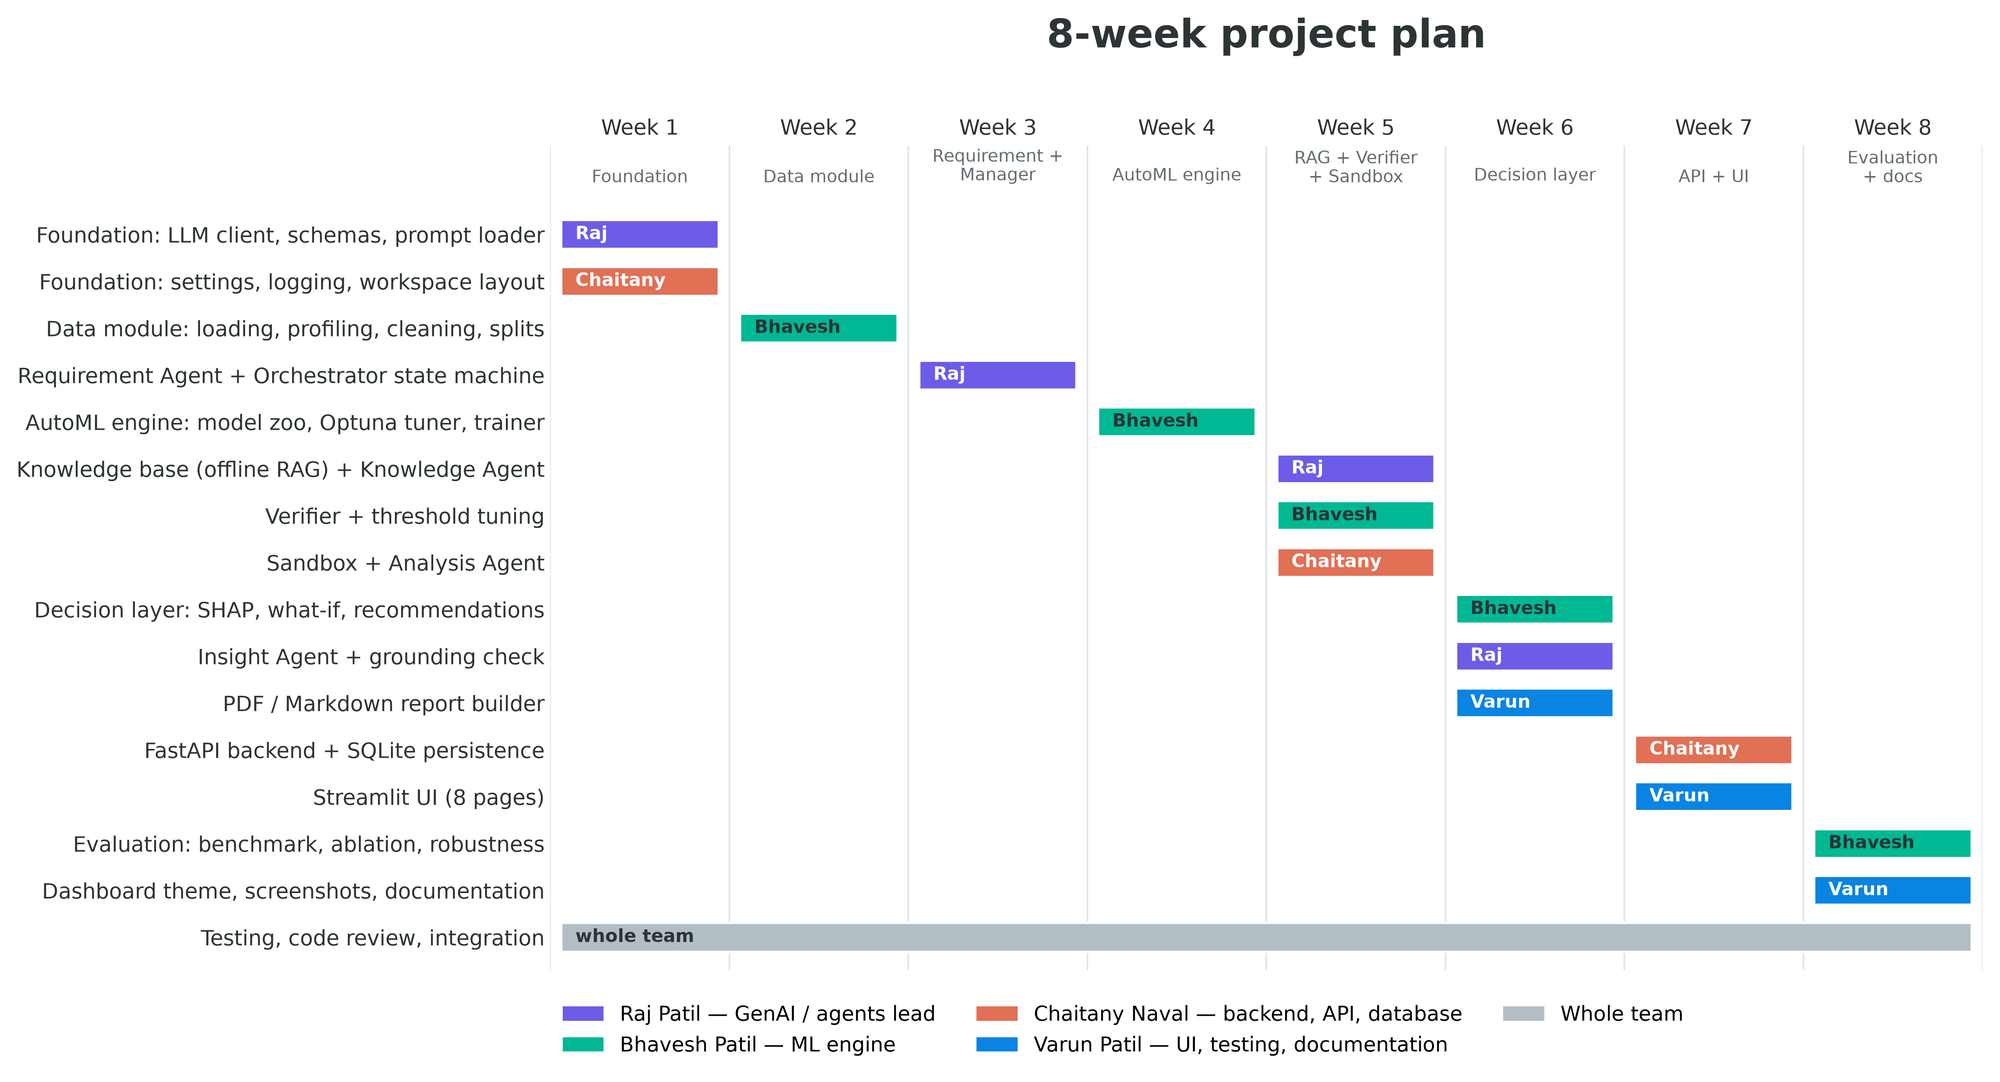
\includegraphics[width=\linewidth,height=7.3in,keepaspectratio]{figures/eight_week_timeline.png}
  \caption{Eight-week project plan (Gantt chart)}\label{fig:3.1}
\end{figure}

\begingroup
\linespread{1}\small
\setlength{\tabcolsep}{4pt}
\begin{longtable}{|>{\raggedright\arraybackslash\hspace{0pt}}p{\dimexpr 0.0869\linewidth-2\tabcolsep-2\arrayrulewidth\relax}|>{\raggedright\arraybackslash\hspace{0pt}}p{\dimexpr 0.2565\linewidth-2\tabcolsep-2\arrayrulewidth\relax}|>{\raggedright\arraybackslash\hspace{0pt}}p{\dimexpr 0.3616\linewidth-2\tabcolsep-2\arrayrulewidth\relax}|>{\raggedright\arraybackslash\hspace{0pt}}p{\dimexpr 0.2950\linewidth-2\tabcolsep-2\arrayrulewidth\relax}|}
\caption{Project schedule and milestones}\label{tab:3.3}\\
\hline
\rowcolor{tableheader}\textbf{Week} & \textbf{Milestone} & \textbf{Key tasks} & \textbf{Closing evidence} \\
\hline
\endfirsthead
\hline
\rowcolor{tableheader}\textbf{Week} & \textbf{Milestone} & \textbf{Key tasks} & \textbf{Closing evidence} \\
\endhead
W1 & Foundation & Settings, logging, LLM client, schemas, prompt loader, test harness & Foundation tests; commits \code{146b1cf}, \code{417219c} \\ \hline
W2 & Data module & Loader, profiler, cleaning, 70/20/10 splits, preprocessing; sample datasets & Data tests; commit \code{cd2b765} \\ \hline
W3 & Requirement Agent + Orchestrator & Relevance, parsing, repair, clarifying questions; resumable state machine & Live LLM demo; commit \code{53ce937} \\ \hline
W4 & AutoML engine & Model zoo, Optuna tuner, evaluator, trainer, Model Agent & Step 4 benchmark; commit \code{9f8d017} \\ \hline
W5 & RAG + Verifier + Sandbox & Knowledge index and agent; threshold tuning; seven checks; sandbox & Updated benchmark; commit \code{eea311a} \\ \hline
W6 & Decision layer & SHAP, what-if, recommender, grounded insight, PDF / Markdown report & Two offline end-to-end runs; commit \code{aa24eed} \\ \hline
W7 & FastAPI + Streamlit UI & 17-endpoint API, worker, SQLite; eight UI pages & API and UI tests; commits \code{29007c0}, \code{7f13403} \\ \hline
W8 & Evaluation + documentation & Benchmark, ablation, robustness; diagrams, manuals; theme, screenshots & \code{evaluation.md}; commits \code{a3aefd2}, \code{3965778} \\ \hline
\end{longtable}
\endgroup

\FloatBarrier
\section{Effort Allocation and Cost Estimation}\label{sec:3.3}

\subsection{Effort Allocation}\label{sec:3.3.1}

Each member led one area of the system (Table~\ref{tab:3.4}); testing, review and integration were shared. Table~\ref{tab:3.5} gives the \textbf{planned} split of work per member and week. It was derived from the roles of Table~\ref{tab:3.4} and the weekly milestones of Table~\ref{tab:3.3}, with an equal share for every member: one person-week per member per week, so 8 person-weeks per member and 32 person-weeks in total.

\begin{table}[H]
\centering
\linespread{1}\small
\setlength{\tabcolsep}{4pt}
\caption{Team roles}\label{tab:3.4}
\begin{tabular}{|>{\raggedright\arraybackslash\hspace{0pt}}p{\dimexpr 0.2240\linewidth-2\tabcolsep-2\arrayrulewidth\relax}|>{\raggedright\arraybackslash\hspace{0pt}}p{\dimexpr 0.2041\linewidth-2\tabcolsep-2\arrayrulewidth\relax}|>{\raggedright\arraybackslash\hspace{0pt}}p{\dimexpr 0.5718\linewidth-2\tabcolsep-2\arrayrulewidth\relax}|}
\hline
\rowcolor{tableheader}\textbf{Member} & \textbf{Role} & \textbf{Main areas} \\
\hline
Raj Vishwas Patil & GenAI / Agents Lead & LLM client, prompts, Requirement, Knowledge, Model and Insight agents \\ \hline
Bhavesh Vinod Patil & ML Engine & Data module, model zoo, tuner, trainer, Verifier, explanations, recommender, evaluation \\ \hline
Chaitany Rajesh Naval & Backend / API / DB & Settings, logging, state persistence, sandbox, FastAPI, worker, SQLite \\ \hline
Varun Darshan Patil & UI / Testing / Docs & Test harness, samples, report builder, Streamlit UI, theme, documentation \\ \hline
\end{tabular}
\end{table}

\begingroup
\linespread{1}\small
\setlength{\tabcolsep}{4pt}
\begin{longtable}{|>{\raggedright\arraybackslash\hspace{0pt}}p{\dimexpr 0.1005\linewidth-2\tabcolsep-2\arrayrulewidth\relax}|>{\raggedright\arraybackslash\hspace{0pt}}p{\dimexpr 0.2141\linewidth-2\tabcolsep-2\arrayrulewidth\relax}|>{\raggedright\arraybackslash\hspace{0pt}}p{\dimexpr 0.2401\linewidth-2\tabcolsep-2\arrayrulewidth\relax}|>{\raggedright\arraybackslash\hspace{0pt}}p{\dimexpr 0.2174\linewidth-2\tabcolsep-2\arrayrulewidth\relax}|>{\raggedright\arraybackslash\hspace{0pt}}p{\dimexpr 0.2278\linewidth-2\tabcolsep-2\arrayrulewidth\relax}|}
\caption{Planned effort allocation per member per week (one person-week per cell)}\label{tab:3.5}\\
\hline
\rowcolor{tableheader}\textbf{Week} & \textbf{Raj Vishwas Patil} & \textbf{Bhavesh Vinod Patil} & \textbf{Chaitany Rajesh Naval} & \textbf{Varun Darshan Patil} \\
\hline
\endfirsthead
\hline
\rowcolor{tableheader}\textbf{Week} & \textbf{Raj Vishwas Patil} & \textbf{Bhavesh Vinod Patil} & \textbf{Chaitany Rajesh Naval} & \textbf{Varun Darshan Patil} \\
\endhead
W1 & LLM client, schemas, prompt loader & Library selection for data and ML & Settings, logging, workspace layout & pytest harness and fixtures \\ \hline
W2 & Data Agent summary prompt and fallback & Loader, profiler, splits, preprocessing & Run ids and run folders & Sample datasets, data tests \\ \hline
W3 & Requirement Agent and prompts & Task metrics, target / task suggestions & State machine persistence, resume & State-machine tests, demo script \\ \hline
W4 & Model Agent and constraint parsing & Model zoo, tuner, evaluator, trainer & TRAIN state integration, artefacts & AutoML tests, benchmark report \\ \hline
W5 & Knowledge notes, index, Knowledge Agent & Verifier, threshold tuning, baselines & Sandbox, Analysis Agent & Retrieval, verifier and sandbox tests \\ \hline
W6 & Insight Agent and grounding check & SHAP, what-if, recommender & EXPLAIN / INSIGHT / REPORT states & PDF / Markdown report builder \\ \hline
W7 & Ask Your Data and LLM-optional API paths & Result endpoints (explanations, what-if) & FastAPI app, worker, SQLite repository & Streamlit UI, API client, page tests \\ \hline
W8 & Evaluation review, report writing & Evaluation script and studies & Lint / coverage set-up, run scripts, API docs & Theme, screenshots, user manual, diagrams \\ \hline
\textbf{Total} & \textbf{8 person-weeks} & \textbf{8 person-weeks} & \textbf{8 person-weeks} & \textbf{8 person-weeks} \\ \hline
\end{longtable}
\endgroup

Four members working for eight weeks gives 32 person-weeks, about 7.4 person-months at 4.33 weeks per month --- in round figures, 4 members \ensuremath{\times} about 2 months \ensuremath{\approx} 8 person-months of actual effort.

\subsection{Size of the Software}\label{sec:3.3.2}

We wrote \code{scripts/\allowbreak{}count\_\allowbreak{}loc.\allowbreak{}py}, which reads every Python file with Python's tokenizer and counts a line as code when it holds at least one token that is not a comment or a docstring; the read-only reference folder and the virtual environment are excluded (Table~\ref{tab:3.6}).

\begin{table}[H]
\centering
\linespread{1}\small
\setlength{\tabcolsep}{4pt}
\caption{Source lines of code (Python)}\label{tab:3.6}
\begin{tabular}{|>{\raggedright\arraybackslash\hspace{0pt}}p{\dimexpr 0.5780\linewidth-2\tabcolsep-2\arrayrulewidth\relax}|>{\raggedleft\arraybackslash\hspace{0pt}}p{\dimexpr 0.1005\linewidth-2\tabcolsep-2\arrayrulewidth\relax}|>{\raggedleft\arraybackslash\hspace{0pt}}p{\dimexpr 0.1809\linewidth-2\tabcolsep-2\arrayrulewidth\relax}|>{\raggedleft\arraybackslash\hspace{0pt}}p{\dimexpr 0.1405\linewidth-2\tabcolsep-2\arrayrulewidth\relax}|}
\hline
\rowcolor{tableheader}\textbf{Package} & \textbf{Files} & \textbf{Physical lines} & \textbf{Code lines} \\
\hline
\code{idss/} (agents, ML engine, decision layer, knowledge, sandbox, storage) & 40 & 7,463 & 5,751 \\ \hline
\code{api/} (FastAPI backend) & 4 & 803 & 573 \\ \hline
\code{ui/} (Streamlit interface) & 15 & 2,278 & 1,719 \\ \hline
\code{configs/} (settings) & 2 & 87 & 61 \\ \hline
\code{scripts/} (evaluation, samples, diagrams, demos) & 8 & 3,180 & 2,579 \\ \hline
\textbf{Delivered code (without tests)} & \textbf{69} & \textbf{13,811} & \textbf{10,683} \\ \hline
\code{tests/} (reported separately) & 15 & 3,938 & 2,983 \\ \hline
\end{tabular}
\end{table}

The application (\code{idss}, \code{api}, \code{ui}, \code{configs}) has 8,104 code lines; with the scripts the delivered code is \textbf{10.683 KLOC}.

\subsection{Cost Estimation with Basic COCOMO}\label{sec:3.3.3}

We used basic COCOMO \cite{ref16} in \textbf{organic mode} (a small team, familiar kind of software, flexible requirements):

\begin{quote}
\textit{E} = 2.4 \ensuremath{\cdot} (KLOC)\textsuperscript{1.05} person-months, \textit{D} = 2.5 \ensuremath{\cdot} \textit{E}\textsuperscript{0.38} months, \textit{P} = \textit{E} / \textit{D} persons.
\end{quote}

For KLOC = 10.683: \textit{E} = 2.4 \ensuremath{\times} 10.683\textsuperscript{1.05} = \textbf{28.86 person-months}, \textit{D} = 2.5 \ensuremath{\times} 28.86\textsuperscript{0.38} = \textbf{8.97 months} and \textit{P} = 28.86 / 8.97 = \textbf{3.22 persons}. Table~\ref{tab:3.7} compares the estimates with the actual effort.

\begin{table}[H]
\centering
\linespread{1}\small
\setlength{\tabcolsep}{4pt}
\caption{Basic COCOMO (organic) estimate and actual effort}\label{tab:3.7}
\begin{tabular}{|>{\raggedright\arraybackslash\hspace{0pt}}p{\dimexpr 0.2543\linewidth-2\tabcolsep-2\arrayrulewidth\relax}|>{\raggedleft\arraybackslash\hspace{0pt}}p{\dimexpr 0.2333\linewidth-2\tabcolsep-2\arrayrulewidth\relax}|>{\raggedleft\arraybackslash\hspace{0pt}}p{\dimexpr 0.2088\linewidth-2\tabcolsep-2\arrayrulewidth\relax}|>{\raggedleft\arraybackslash\hspace{0pt}}p{\dimexpr 0.3035\linewidth-2\tabcolsep-2\arrayrulewidth\relax}|}
\hline
\rowcolor{tableheader}\textbf{Quantity} & \textbf{Application only (8.104 KLOC)} & \textbf{Delivered code (10.683 KLOC)} & \textbf{Actual project} \\
\hline
Effort \textit{E} (person-months) & 21.59 & 28.86 & \ensuremath{\approx} 8 (4 members \ensuremath{\times} \textasciitilde{}2 months; 32 person-weeks = 7.4) \\ \hline
Duration \textit{D} (months) & 8.04 & 8.97 & \ensuremath{\approx} 1.8 (8 weeks) \\ \hline
Average staff \textit{P} (persons) & 2.69 & 3.22 & 4 \\ \hline
\end{tabular}
\end{table}

\textbf{Why the actual effort is lower than the estimate.} COCOMO estimates 28.86 person-months for the delivered code, while the actual effort was about 8 person-months (4 members \ensuremath{\times} about 2 months), roughly 3.6 times less. We report this difference instead of adjusting the estimate. Basic COCOMO assumes traditional development in which every line is designed, written and debugged by hand; it was calibrated on industrial projects of the late 1970s \cite{ref16} and assumes a full industrial lifecycle with formal reviews, documentation and maintenance that a fixed-scope student project does not have. Our project differed in two ways. First, it reuses mature open-source libraries heavily: training, tuning, SHAP, the web server, the UI, the database and PDF generation are not our code. Second, we used an AI coding assistant (Claude Code) to help generate and refactor code, which shortened the time from a design decision to working, tested code; the design, integration, testing and evaluation were still carried out and verified by the team. The COCOMO figure is therefore best read as the effort the same code would need if it were written entirely by hand, and as confirmation that the scope was ambitious for eight weeks.

\subsection{Actual Cost}\label{sec:3.3.4}

\begin{table}[H]
\centering
\linespread{1}\small
\setlength{\tabcolsep}{4pt}
\caption{Actual cost}\label{tab:3.8}
\begin{tabular}{|>{\raggedright\arraybackslash\hspace{0pt}}p{\dimexpr 0.3840\linewidth-2\tabcolsep-2\arrayrulewidth\relax}|>{\raggedright\arraybackslash\hspace{0pt}}p{\dimexpr 0.2533\linewidth-2\tabcolsep-2\arrayrulewidth\relax}|>{\raggedright\arraybackslash\hspace{0pt}}p{\dimexpr 0.3626\linewidth-2\tabcolsep-2\arrayrulewidth\relax}|}
\hline
\rowcolor{tableheader}\textbf{Resource} & \textbf{Use} & \textbf{Cost} \\
\hline
Python and open-source libraries (pandas, scikit-learn, XGBoost, LightGBM, Optuna, SHAP, FastAPI, Streamlit, SQLAlchemy, reportlab, matplotlib, pytest, ruff, Playwright) & Development, testing, evaluation & \rupee{}0 (open-source licences) \\ \hline
Git, SQLite & Version control, database & \rupee{}0 (open-source licences) \\ \hline
Team laptops (Windows) & Development and evaluation & \rupee{}0 (already owned) \\ \hline
LLM API (OpenAI-compatible) & Optional language tasks & Within the provider's free tier; the tests and the evaluation use no LLM \\ \hline
\end{tabular}
\end{table}

The software licence cost of the project is therefore \rupee{}0, and LLM usage stayed within the free tier of the provider.

\FloatBarrier
\section{Summary}\label{sec:3.4}

The project was technically, economically, operationally and schedule-wise feasible with a strict scope. Twelve risks --- including LLM unavailability, hallucinated numbers, unsafe code, data leakage and usage limits --- were identified and mitigated in the final system. The work was scheduled as eight weekly increments and divided among four members by area. Basic COCOMO on the real code size (10.683 KLOC) estimates 28.86 person-months, about 3.6 times the roughly 8 person-months actually spent, because COCOMO assumes manual development while we reused open-source libraries and used an AI coding assistant; the licence cost was \rupee{}0 and LLM usage stayed within the free tier.

% Generated by scripts/build_latex.py from docs/report/ch4_analysis_design.md: edit the Markdown, not this file.
\chapter{System Analysis and Design}\label{ch:4}

This chapter specifies what IDSS must do --- functional, non-functional, data, hardware and software requirements, summarised as an SRS --- and how it is designed: the architecture, the data flow diagrams, the UML diagrams and the database.

\FloatBarrier
\section{Requirement Collection and Identification}\label{sec:4.1}

\subsection{Requirement Collection}\label{sec:4.1.1}

Requirements came from four sources: (1) the project brief discussed with our guide --- a system in which a user states a business problem in plain language and receives a validated model with explained, actionable decisions; (2) the literature, especially AutoML-Agent \cite{ref9} (Chapter~\ref{ch:2}); (3) five representative business scenarios --- customer churn, crop price, daily store sales, delivery delays and customer segments --- for which we generated synthetic datasets and walked through each question from the user's side; and (4) the risks of LLM-based systems (Section~\ref{sec:3.1.2}), which became non-functional requirements. The stakeholders are the \textbf{business user}, who needs answers without programming; the \textbf{team member or evaluator}, who runs tests, the evaluation and the tooling; the \textbf{guide and examiners}, who need evidence that results are correct and honestly verified; and the \textbf{LLM provider}, an optional external system that receives aggregates only.

\subsection{Functional Requirements}\label{sec:4.1.2}

\begingroup
\linespread{1}\small
\setlength{\tabcolsep}{4pt}
\begin{longtable}{|>{\raggedright\arraybackslash\hspace{0pt}}p{\dimexpr 0.1005\linewidth-2\tabcolsep-2\arrayrulewidth\relax}|>{\raggedright\arraybackslash\hspace{0pt}}p{\dimexpr 0.5708\linewidth-2\tabcolsep-2\arrayrulewidth\relax}|>{\raggedright\arraybackslash\hspace{0pt}}p{\dimexpr 0.3286\linewidth-2\tabcolsep-2\arrayrulewidth\relax}|}
\caption{Functional requirements}\label{tab:4.1}\\
\hline
\rowcolor{tableheader}\textbf{ID} & \textbf{The system shall \ldots{}} & \textbf{Implemented in} \\
\hline
\endfirsthead
\hline
\rowcolor{tableheader}\textbf{ID} & \textbf{The system shall \ldots{}} & \textbf{Implemented in} \\
\endhead
FR-01 & accept CSV, Excel, JSON or Parquet files of at most 50 MB, store them under a sanitised name and list them & \code{api/\allowbreak{}main.py}, \code{data\_\allowbreak{}loader.py} \\ \hline
FR-02 & profile each dataset: types, missing values, distinct counts, suggested target and task, leakage and imbalance warnings & \code{profiler.py} \\ \hline
FR-03 & check whether a question can be answered from data and reply politely, without training, when it cannot & Requirement Agent \\ \hline
FR-04 & convert the question into a structured requirement and repair it against the data profile & Requirement Agent \\ \hline
FR-05 & ask clarifying questions when information is missing (at most two rounds) and continue with the answers & Requirement Agent, Orchestrator \\ \hline
FR-06 & clean the data and split it 70/20/10 (stratified, or chronological for time series) & \code{preprocess.py}, Data Agent \\ \hline
FR-07 & retrieve best-practice knowledge and plan models only from a fixed zoo, honouring latency, training-time and explainability constraints & Knowledge and Model agents \\ \hline
FR-08 & tune candidates within the budget, select on the validation split, tune the decision threshold (binary), refit and evaluate once on the test split with a baseline & \code{tuner.py}, \code{trainer.py} \\ \hline
FR-09 & verify results with rule-based checks, re-plan once on failure and flag results that still fail & Verifier, Orchestrator \\ \hline
FR-10 & explain the model globally and per record in the original column names & \code{explain.py} \\ \hline
FR-11 & simulate what-if changes for a record and for a filtered segment, validated against the profile & \code{what\_\allowbreak{}if.py} \\ \hline
FR-12 & produce risk tiers and counterfactual actions, lever effects, forecasts with an interval or segment profiles & \code{recommender.py}, \code{explain.py} \\ \hline
FR-13 & write a decision brief whose numbers all appear in the computed facts & Insight Agent \\ \hline
FR-14 & generate downloadable PDF and Markdown reports with charts & \code{report\_\allowbreak{}builder.py} \\ \hline
FR-15 & answer ad-hoc data questions with LLM-written code run in a sandbox (LLM required) & Analysis Agent, sandbox \\ \hline
FR-16 & show run progress (state, percentage, events) and resume runs after a restart & Orchestrator, Run Monitor \\ \hline
FR-17 & store datasets, runs and events in a database and list and filter runs & \code{idss/\allowbreak{}storage/} \\ \hline
FR-18 & expose every function through a REST API with a uniform error format & \code{api/} \\ \hline
FR-19 & complete the whole pipeline without an LLM & Every agent's fallback \\ \hline
FR-20 & offer a one-click demonstration on a sample dataset & Home page (Demo Mode) \\ \hline
\end{longtable}
\endgroup

\subsection{Non-functional Requirements}\label{sec:4.1.3}

\begingroup
\linespread{1}\small
\setlength{\tabcolsep}{4pt}
\begin{longtable}{|>{\raggedright\arraybackslash\hspace{0pt}}p{\dimexpr 0.1142\linewidth-2\tabcolsep-2\arrayrulewidth\relax}|>{\raggedright\arraybackslash\hspace{0pt}}p{\dimexpr 0.2456\linewidth-2\tabcolsep-2\arrayrulewidth\relax}|>{\raggedright\arraybackslash\hspace{0pt}}p{\dimexpr 0.6403\linewidth-2\tabcolsep-2\arrayrulewidth\relax}|}
\caption{Non-functional requirements}\label{tab:4.2}\\
\hline
\rowcolor{tableheader}\textbf{ID} & \textbf{Category} & \textbf{Requirement} \\
\hline
\endfirsthead
\hline
\rowcolor{tableheader}\textbf{ID} & \textbf{Category} & \textbf{Requirement} \\
\endhead
NFR-01 & Performance & Fast budget: \ensuremath{\leq} 3 models \ensuremath{\times} 15 trials, \ensuremath{\leq} 60 s per model, \ensuremath{\leq} 180 s in total; the UI refreshes progress every 2 s \\ \hline
NFR-02 & Reliability & Every LLM call has a timeout and \ensuremath{\leq} 3 retries with backoff; a failing step ends the run in FAILED, never crashes it \\ \hline
NFR-03 & Bounded behaviour & \ensuremath{\leq} 2 clarification rounds, 1 re-plan and 50 steps per call; one training run at a time \\ \hline
NFR-04 & Degradation & Every agent has a deterministic fallback; the system works without an LLM \\ \hline
NFR-05 & Privacy & Prompts carry names, types, aggregates, metrics and facts only --- never raw rows, paths or keys; localhost only \\ \hline
NFR-06 & Security & Keys only in \code{.env}; LLM code only in the sandbox; uploads, ids and paths validated \\ \hline
NFR-07 & Validity & Test split read exactly once; baselines on the same split; reproducible with a seed \\ \hline
NFR-08 & Transparency & Recommendations carry evidence; repairs, checks and tier cut-offs are shown \\ \hline
NFR-09 & Usability & A non-programmer completes an analysis in the browser; clear empty states and backend-down messages \\ \hline
NFR-10 & Durability & Run state saved atomically after every transition; a database error never stops a run \\ \hline
NFR-11 & Maintainability & Type hints, Pydantic v2 schemas at module boundaries, modular packages, linting, one logger \\ \hline
NFR-12 & Testability & An automated test suite that runs offline without network calls \\ \hline
NFR-13 & Portability & Windows 10 / 11, Python 3.12; any OpenAI-compatible provider or local Ollama \\ \hline
\end{longtable}
\endgroup

\subsection{Data and Behavioural Requirements}\label{sec:4.1.4}

\begin{table}[H]
\centering
\linespread{1}\small
\setlength{\tabcolsep}{4pt}
\caption{Data requirements}\label{tab:4.3}
\begin{tabular}{|>{\raggedright\arraybackslash\hspace{0pt}}p{\dimexpr 0.2614\linewidth-2\tabcolsep-2\arrayrulewidth\relax}|>{\raggedright\arraybackslash\hspace{0pt}}p{\dimexpr 0.7386\linewidth-2\tabcolsep-2\arrayrulewidth\relax}|}
\hline
\rowcolor{tableheader}\textbf{Item} & \textbf{Requirement} \\
\hline
Structure and format & One table with a header row; \code{.csv} (delimiter and encoding detected), \code{.xlsx}, \code{.json} (incl. JSON lines), \code{.parquet} \\ \hline
Size & \ensuremath{\leq} 50 MB; at least 10 rows to split; the Verifier requires \ensuremath{\geq} 30 test rows (10\% of the data) \\ \hline
Target & A numeric, categorical or boolean column with more than one value; identifiers, dates and free text cannot be targets \\ \hline
Time series & A date column and a numeric target; chronological split; features from earlier rows only \\ \hline
Clustering & No target; an optional ground-truth column is used only for scoring \\ \hline
\end{tabular}
\end{table}

The behaviour of a run is the state machine of Section~\ref{sec:4.5.4}: INIT \ensuremath{\rightarrow} PARSE \ensuremath{\rightarrow} VALIDATE \ensuremath{\rightarrow} PROFILE \ensuremath{\rightarrow} PLAN \ensuremath{\rightarrow} TRAIN \ensuremath{\rightarrow} VERIFY \ensuremath{\rightarrow} EXPLAIN \ensuremath{\rightarrow} INSIGHT \ensuremath{\rightarrow} REPORT \ensuremath{\rightarrow} DONE, with NEEDS\_INPUT while waiting for an answer and FAILED on an error.

\subsection{Software Requirements Specification (Summary)}\label{sec:4.1.5}

\begin{itemize}
  \item \textbf{Purpose and users.} IDSS turns a plain-language question and a data table into a verified model, explanations, actions, what-if simulations and a report, for business users (web interface) and technical users (REST API, scripts).
  \item \textbf{Functions and qualities.} FR-01 to FR-20 (Table~\ref{tab:4.1}) and NFR-01 to NFR-13 (Table~\ref{tab:4.2}).
  \item \textbf{Environment.} One Windows 10 / 11 machine with Python 3.12 and a web browser; optionally an OpenAI-compatible LLM endpoint or a local Ollama server.
  \item \textbf{Interfaces.} Eight Streamlit pages; a REST API with 17 endpoints on \code{localhost:8000}; the OpenAI-compatible chat-completions API; files and an SQLite database under \code{workspace/}.
  \item \textbf{Constraints and assumptions.} The LLM never writes training code; secrets only in \code{.env}; retries capped at 3; data fits in memory; one user runs one training at a time.
\end{itemize}

\FloatBarrier
\section{Hardware and Software Requirements}\label{sec:4.2}

Table~\ref{tab:4.4} gives the minimum hardware for running IDSS and, for comparison, the machine on which it was developed and evaluated (details in Table~\ref{tab:5.2}). More CPU cores shorten tuning; no GPU is used.

\begin{table}[H]
\centering
\linespread{1}\small
\setlength{\tabcolsep}{4pt}
\caption{Hardware requirements}\label{tab:4.4}
\begin{tabular}{|>{\raggedright\arraybackslash\hspace{0pt}}p{\dimexpr 0.1819\linewidth-2\tabcolsep-2\arrayrulewidth\relax}|>{\raggedright\arraybackslash\hspace{0pt}}p{\dimexpr 0.4284\linewidth-2\tabcolsep-2\arrayrulewidth\relax}|>{\raggedright\arraybackslash\hspace{0pt}}p{\dimexpr 0.3897\linewidth-2\tabcolsep-2\arrayrulewidth\relax}|}
\hline
\rowcolor{tableheader}\textbf{Component} & \textbf{Minimum requirement} & \textbf{Development machine (used)} \\
\hline
Processor & 64-bit multi-core CPU (4 cores) & Intel Core i7-11800H, 8 cores / 16 logical processors, 2.30 GHz \\ \hline
Memory & 8 GB RAM & 16 GB RAM \\ \hline
Storage & About 5 GB free: the virtual environment takes about 1.2 GB, plus datasets and run folders & 1 TB NVMe SSD \\ \hline
GPU & Not required & NVIDIA GeForce RTX 3050 Ti Laptop GPU (present, not used by IDSS) \\ \hline
Network & Only for package installation, an external LLM or web search & Same \\ \hline
Operating system & Windows 10 / 11, 64-bit & Windows 11 Home Single Language, 64-bit \\ \hline
\end{tabular}
\end{table}

\begingroup
\linespread{1}\small
\setlength{\tabcolsep}{4pt}
\begin{longtable}{|>{\raggedright\arraybackslash\hspace{0pt}}p{\dimexpr 0.3307\linewidth-2\tabcolsep-2\arrayrulewidth\relax}|>{\raggedright\arraybackslash\hspace{0pt}}p{\dimexpr 0.2549\linewidth-2\tabcolsep-2\arrayrulewidth\relax}|>{\raggedright\arraybackslash\hspace{0pt}}p{\dimexpr 0.4144\linewidth-2\tabcolsep-2\arrayrulewidth\relax}|}
\caption{Software requirements}\label{tab:4.5}\\
\hline
\rowcolor{tableheader}\textbf{Software} & \textbf{Version} & \textbf{Purpose} \\
\hline
\endfirsthead
\hline
\rowcolor{tableheader}\textbf{Software} & \textbf{Version} & \textbf{Purpose} \\
\endhead
Windows & 10 / 11 & Operating system (the Python code is portable) \\ \hline
Python & 3.12 & Runtime \\ \hline
pandas, NumPy, PyArrow, openpyxl & 3.0.6, 2.5.3, 25.0.1, 3.1.5 & Data handling \\ \hline
scikit-learn, XGBoost, LightGBM & 1.9.1, 3.4.1, 4.7.0 & Models \\ \hline
Optuna, SHAP & 5.0.0, 0.52.0 & Tuning, explanations \\ \hline
Pydantic, pydantic-settings & 2.13.5, 2.15.0 & Schemas, settings \\ \hline
openai & 3.24.0 & Client for any OpenAI-compatible LLM \\ \hline
FastAPI, Uvicorn & 0.142.2, 0.54.0 & REST API \\ \hline
Streamlit, Plotly, requests & 1.65.0, 7.1.0, 2.34.2 & User interface \\ \hline
SQLAlchemy (SQLite) & 2.1.3 & Persistence \\ \hline
reportlab, matplotlib, loguru & 5.0.1, 3.11.2, 0.7.3 & Reports, charts, logging \\ \hline
Web browser & Current version & Access to \code{http:/\allowbreak{}/\allowbreak{}localhost:8501} \\ \hline
\end{longtable}
\endgroup

\FloatBarrier
\section{System Architecture}\label{sec:4.3}

Figure~\ref{fig:4.1} shows the layered architecture (Table~\ref{tab:4.6}). \textbf{LLM agents plan and explain, deterministic engines compute}, and every layer also works without an LLM. A request flows downwards: the UI calls the API; the API hands the run to the RunWorker thread, which drives the Orchestrator; the Orchestrator calls one agent per state; agents use the engines for all computation and, when configured, the LLM client for language tasks. The architecture keeps the multi-agent decomposition, structured requirements, retrieval-augmented planning and multi-stage verification of AutoML-Agent \cite{ref9}, replaces LLM-written training code with a deterministic engine and adds the decision layer, sandbox, persistence, API and UI (Tables~\ref{tab:2.2} and~\ref{tab:2.3}).

\begin{figure}[htbp]
  \centering
  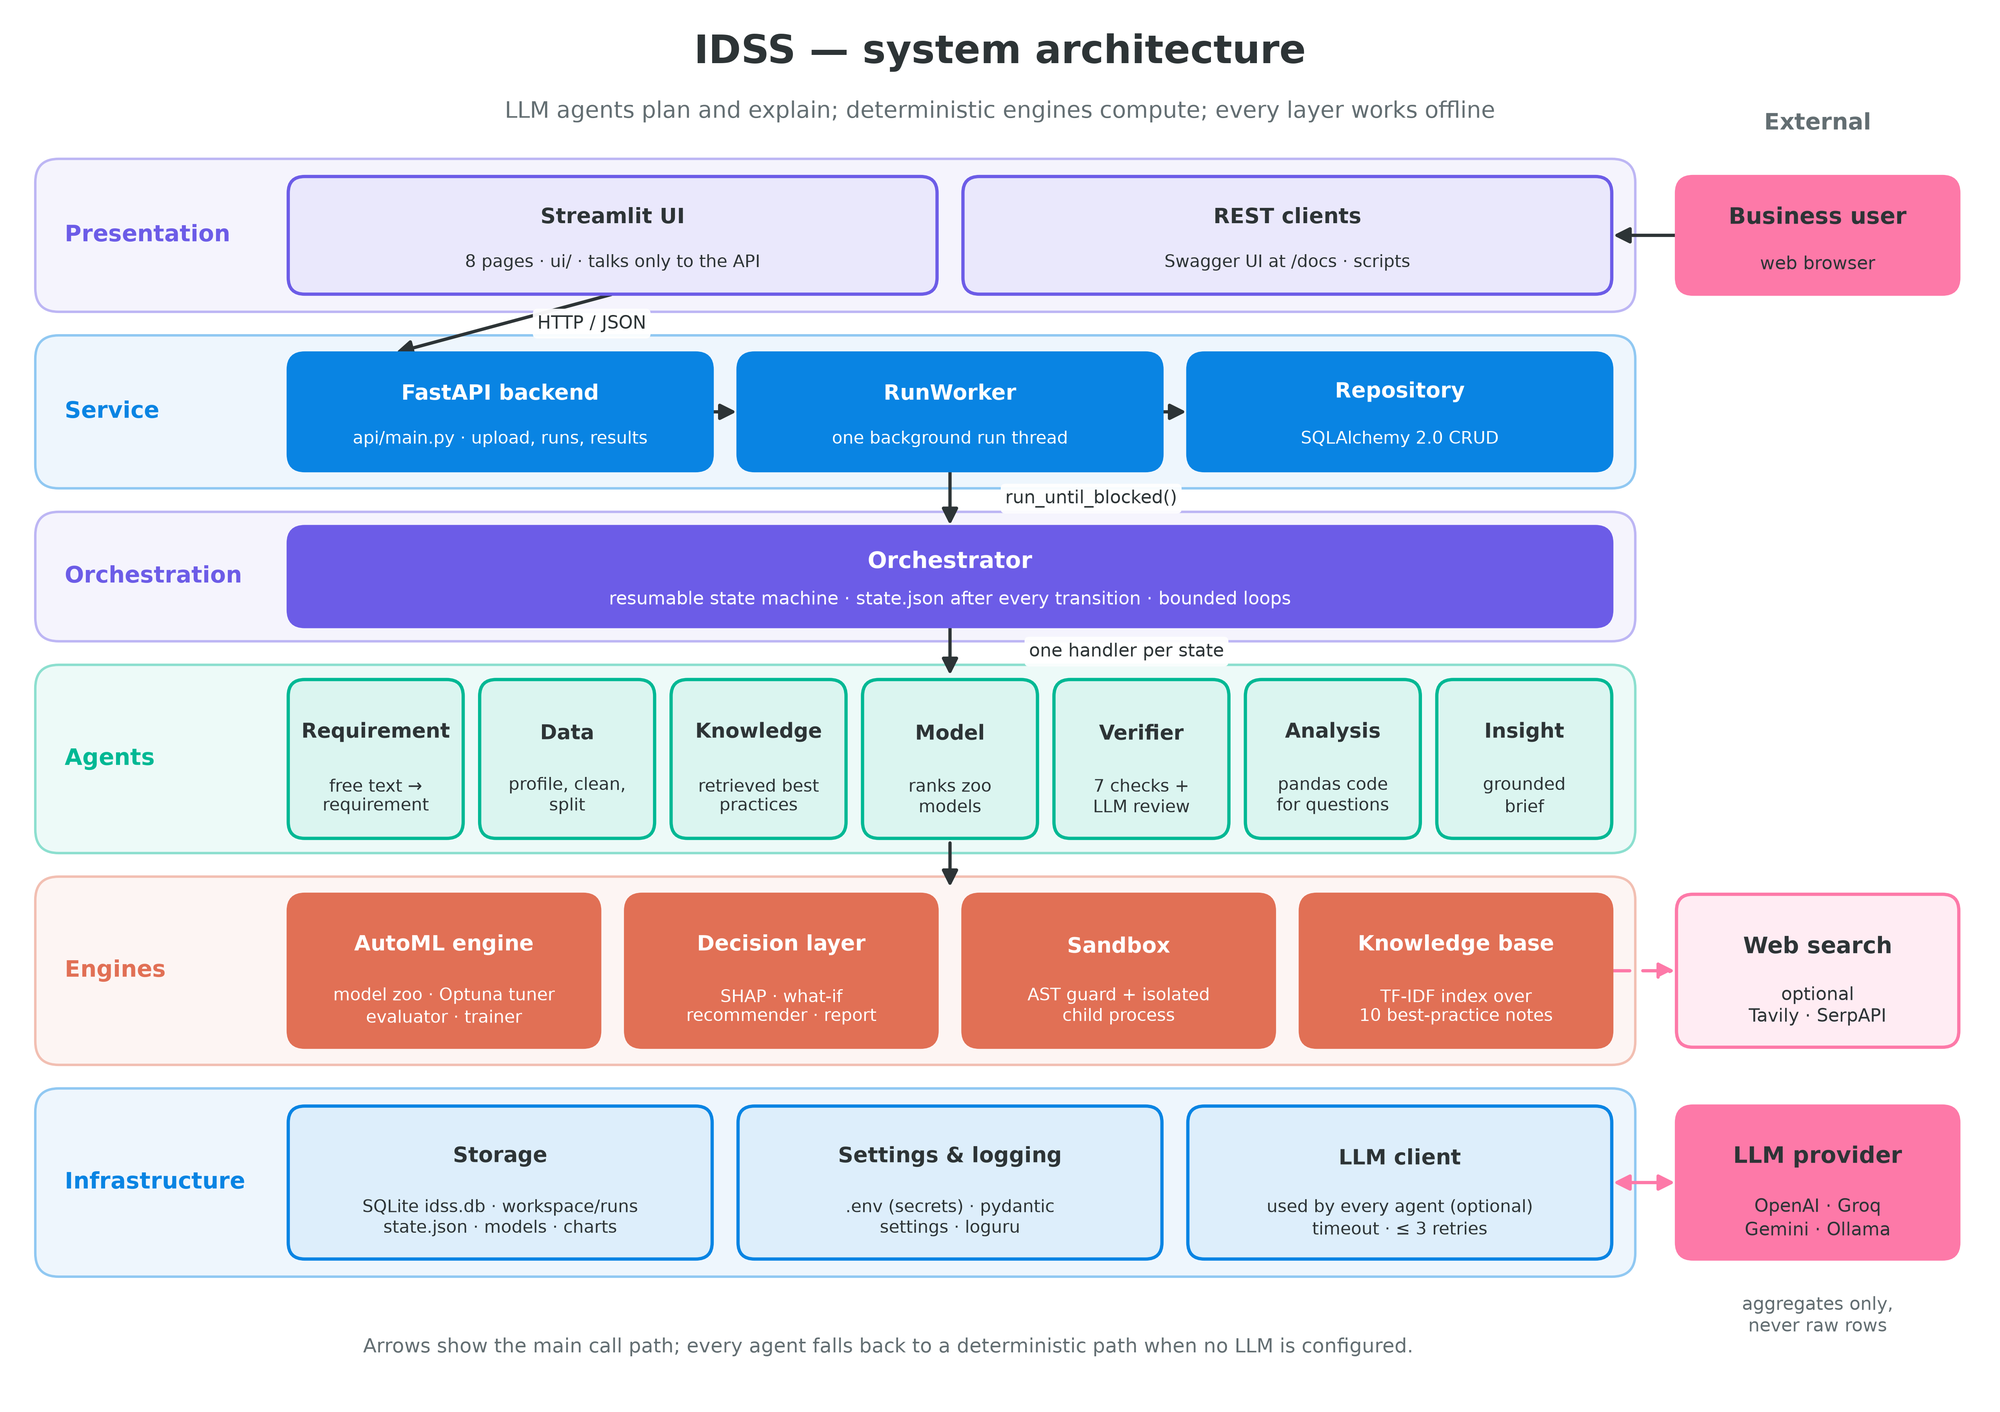
\includegraphics[width=\linewidth,height=7.3in,keepaspectratio]{figures/system_architecture.png}
  \caption{System architecture of IDSS}\label{fig:4.1}
\end{figure}

\begin{table}[H]
\centering
\linespread{1}\small
\setlength{\tabcolsep}{4pt}
\caption{Architectural layers}\label{tab:4.6}
\begin{tabular}{|>{\raggedright\arraybackslash\hspace{0pt}}p{\dimexpr 0.2231\linewidth-2\tabcolsep-2\arrayrulewidth\relax}|>{\raggedright\arraybackslash\hspace{0pt}}p{\dimexpr 0.3897\linewidth-2\tabcolsep-2\arrayrulewidth\relax}|>{\raggedright\arraybackslash\hspace{0pt}}p{\dimexpr 0.3872\linewidth-2\tabcolsep-2\arrayrulewidth\relax}|}
\hline
\rowcolor{tableheader}\textbf{Layer} & \textbf{Components} & \textbf{Code} \\
\hline
Presentation & Streamlit UI (8 pages), talks only to the API & \code{ui/} \\ \hline
Service & FastAPI backend, RunWorker thread, repository & \code{api/}, \code{idss/\allowbreak{}storage/} \\ \hline
Orchestration & Resumable state machine, one handler per state & \code{idss/\allowbreak{}agents/\allowbreak{}manager.\allowbreak{}py} \\ \hline
Agents & Requirement, Data, Knowledge, Model, Verifier, Analysis, Insight & \code{idss/\allowbreak{}agents/} \\ \hline
Engines & AutoML engine, decision layer, knowledge base, sandbox & \code{idss/\allowbreak{}ml/}, \code{idss/\allowbreak{}decision/}, \code{idss/\allowbreak{}knowledge/}, \code{idss/\allowbreak{}execution/} \\ \hline
Infrastructure & LLM client, SQLite and run workspace, settings, logging & \code{idss/\allowbreak{}core/}, \code{idss/\allowbreak{}storage/}, \code{configs/} \\ \hline
\end{tabular}
\end{table}

\FloatBarrier
\section{Data Flow Diagrams}\label{sec:4.4}

\textbf{Level 0.} Figure~\ref{fig:4.2} shows IDSS as one process and its external entities. The business user sends a dataset, a question, answers and what-if changes, and receives the profile, progress, clarifying questions, results, actions and the report. The optional LLM provider receives prompts with aggregates only and returns structured JSON; the optional web search service receives queries and returns snippets. Without an LLM, these flows are skipped.

\begin{figure}[htbp]
  \centering
  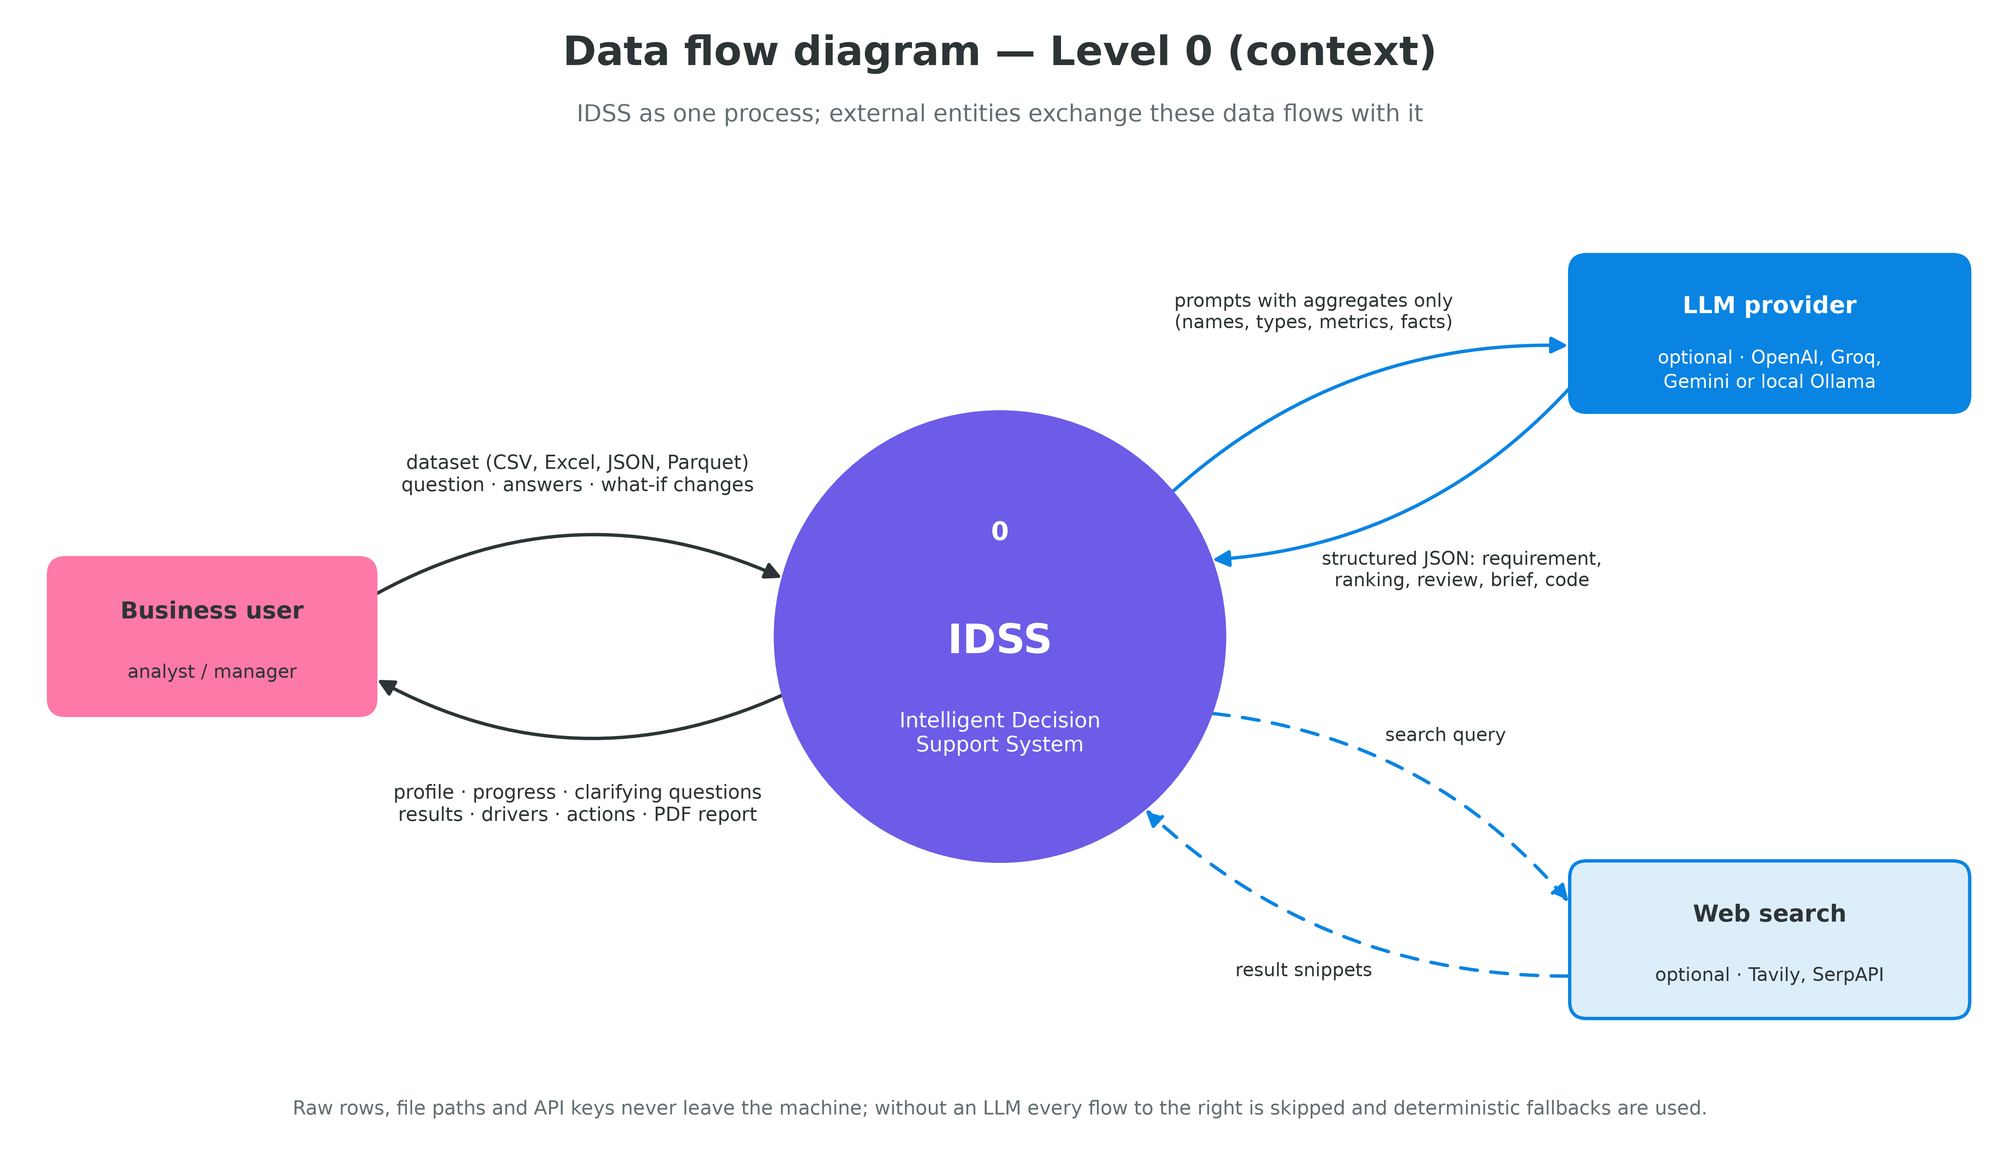
\includegraphics[width=\linewidth,height=7.3in,keepaspectratio]{figures/dfd_level0.png}
  \caption{Data flow diagram, Level 0 (context diagram)}\label{fig:4.2}
\end{figure}

\textbf{Level 1.} Figure~\ref{fig:4.3} decomposes the process. The file is loaded and profiled, cleaned, split 70/20/10 and preprocessed. Candidate models are tuned on the train and validation splits, the best compliant one is selected (with its decision threshold), refitted on train + validation and scored \textbf{once} on the held-out test split with a baseline, then verified and explained. Finally the system derives decisions, writes the grounded insight and builds the report. The run folder stores state, splits, model, charts and reports; SQLite indexes datasets, runs and events.

\begin{figure}[htbp]
  \centering
  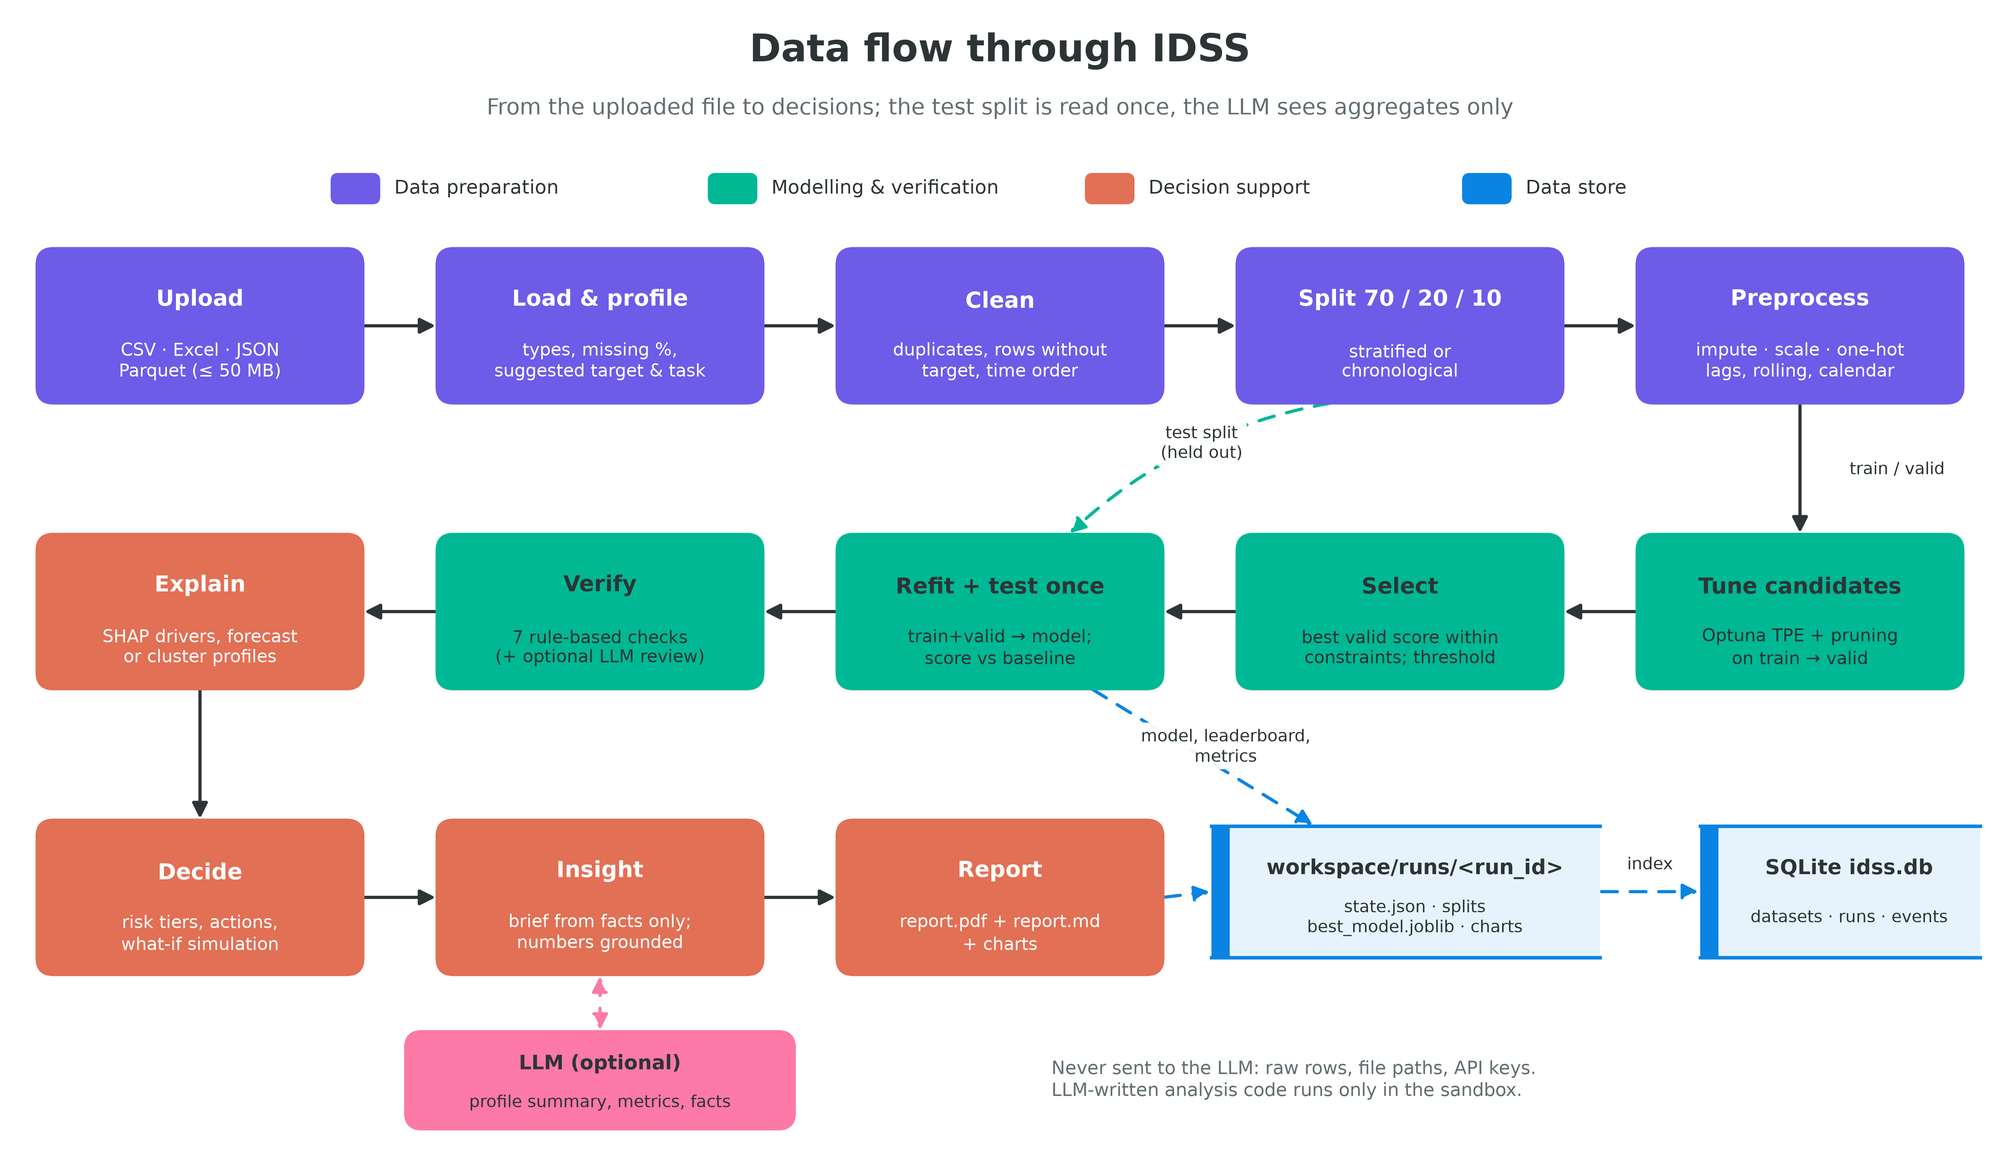
\includegraphics[width=\linewidth,height=7.3in,keepaspectratio]{figures/data_flow.png}
  \caption{Data flow diagram, Level 1}\label{fig:4.3}
\end{figure}

\FloatBarrier
\section{UML Diagrams}\label{sec:4.5}

\subsection{Use Case Diagram}\label{sec:4.5.1}

The business user uploads and profiles data, describes the problem (extended by answering clarifying questions), monitors runs, views results and verification, explores drivers, reviews recommendations and risk tiers, simulates what-if scenarios, asks questions about the data and downloads reports. A team member runs the evaluation and the tests and regenerates samples and diagrams. The LLM provider is an optional external system (Figure~\ref{fig:4.4}).

\begin{figure}[htbp]
  \centering
  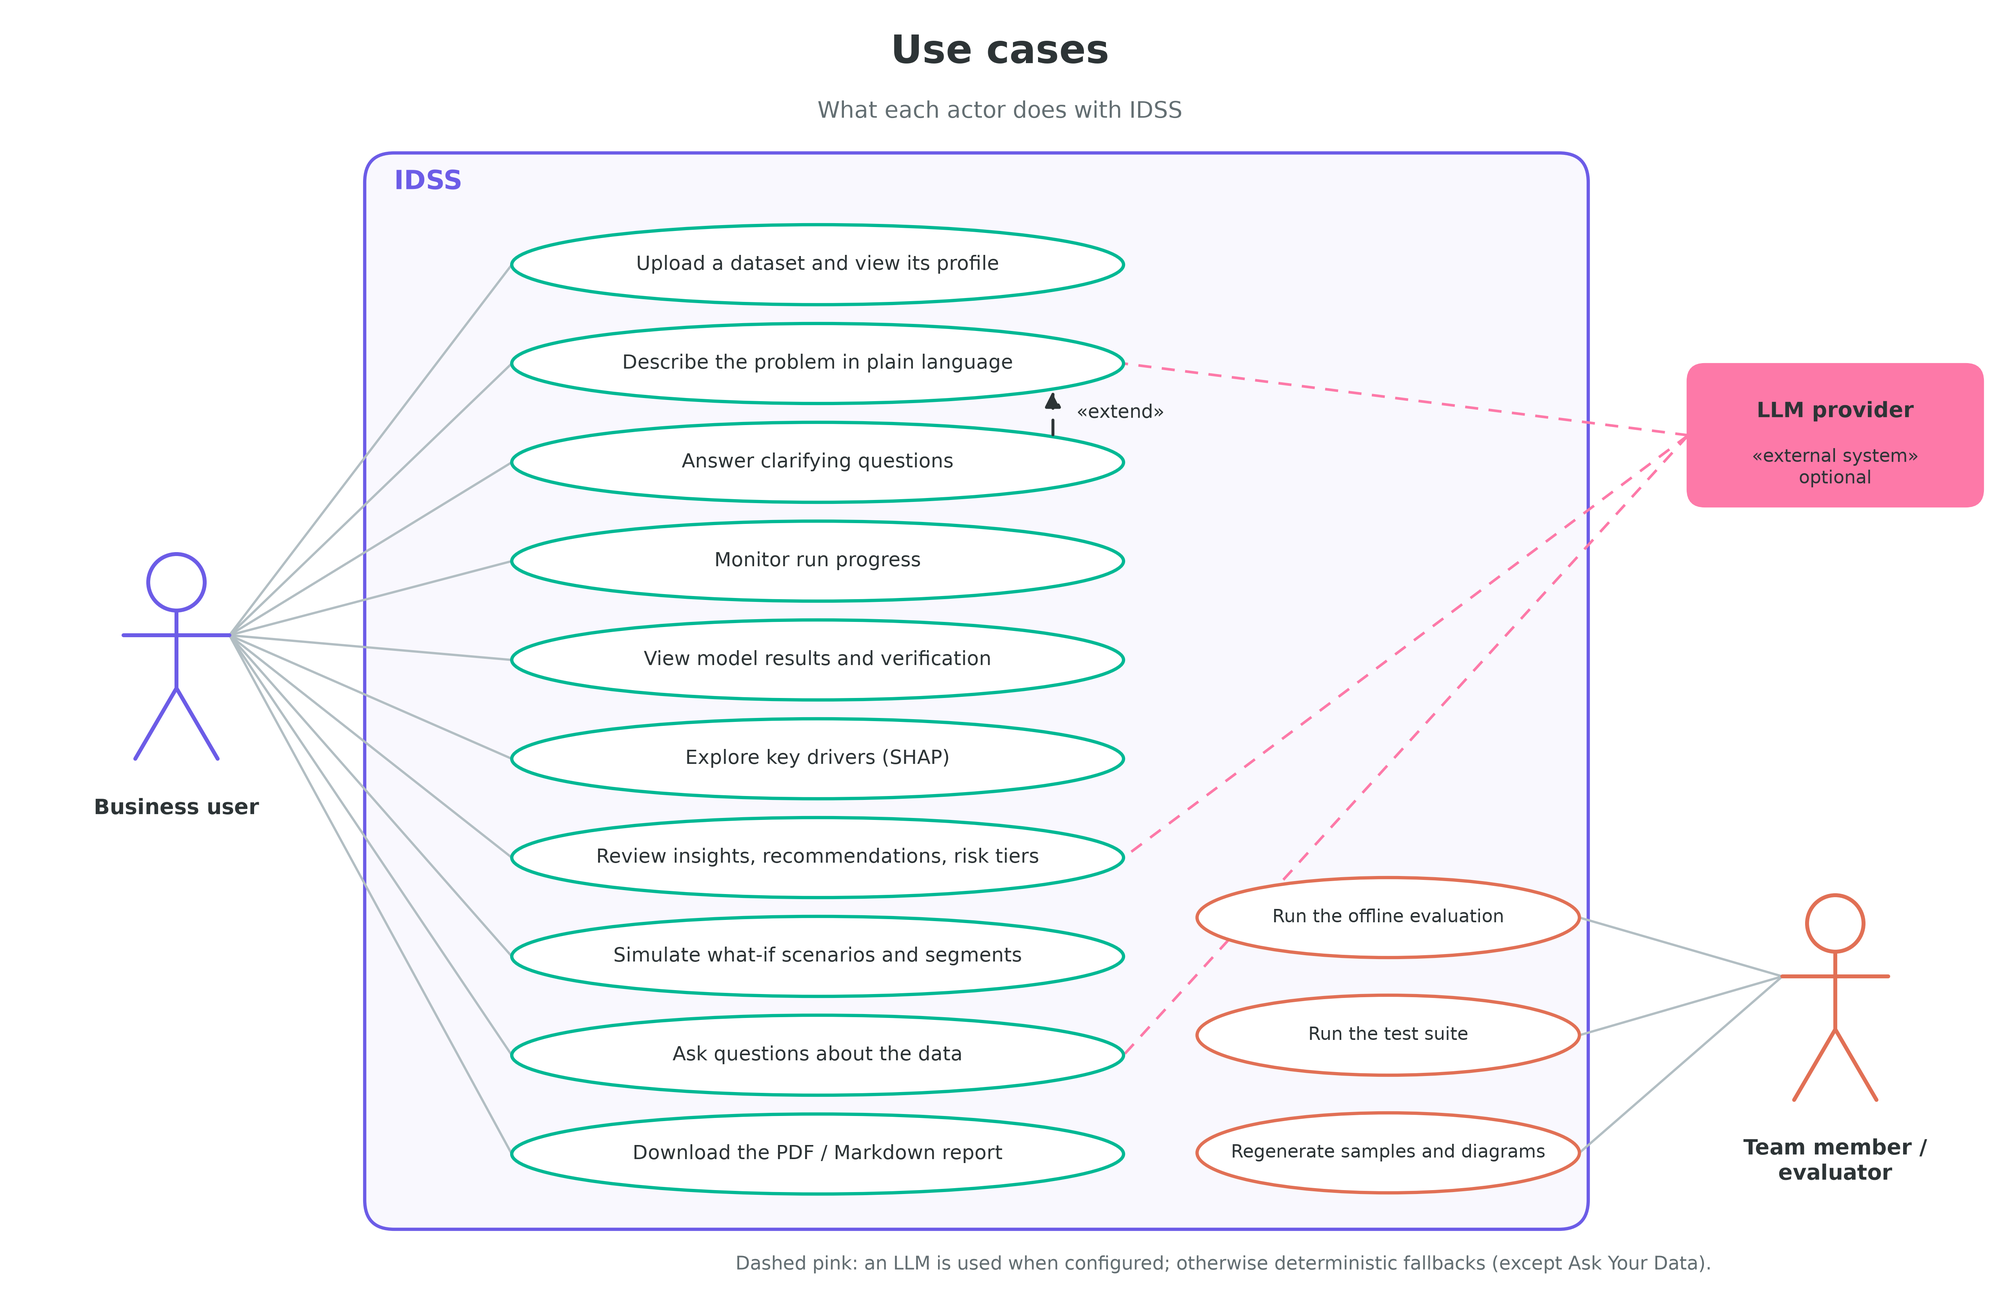
\includegraphics[width=\linewidth,height=7.3in,keepaspectratio]{figures/use_case.png}
  \caption{Use case diagram}\label{fig:4.4}
\end{figure}

\subsection{Class Diagram}\label{sec:4.5.2}

The \textbf{Orchestrator} owns one instance of each agent and the current \textbf{RunContext}, which holds the whole state of a run and is saved as \code{state.json}; it mirrors every transition into the \textbf{Repository} and is driven by the API's \textbf{RunWorker}. Every agent holds an optional \textbf{LLMClient}. The \textbf{KnowledgeAgent} queries the \textbf{KnowledgeIndex}; in the TRAIN state the \textbf{AutoMLTrainer} creates a \textbf{TrainedModel} and reads the test split through the \textbf{Holdout}, whose access log proves a single read; the \textbf{ModelExplainer} explains a TrainedModel (Figure~\ref{fig:4.5}).

\begin{figure}[htbp]
  \centering
  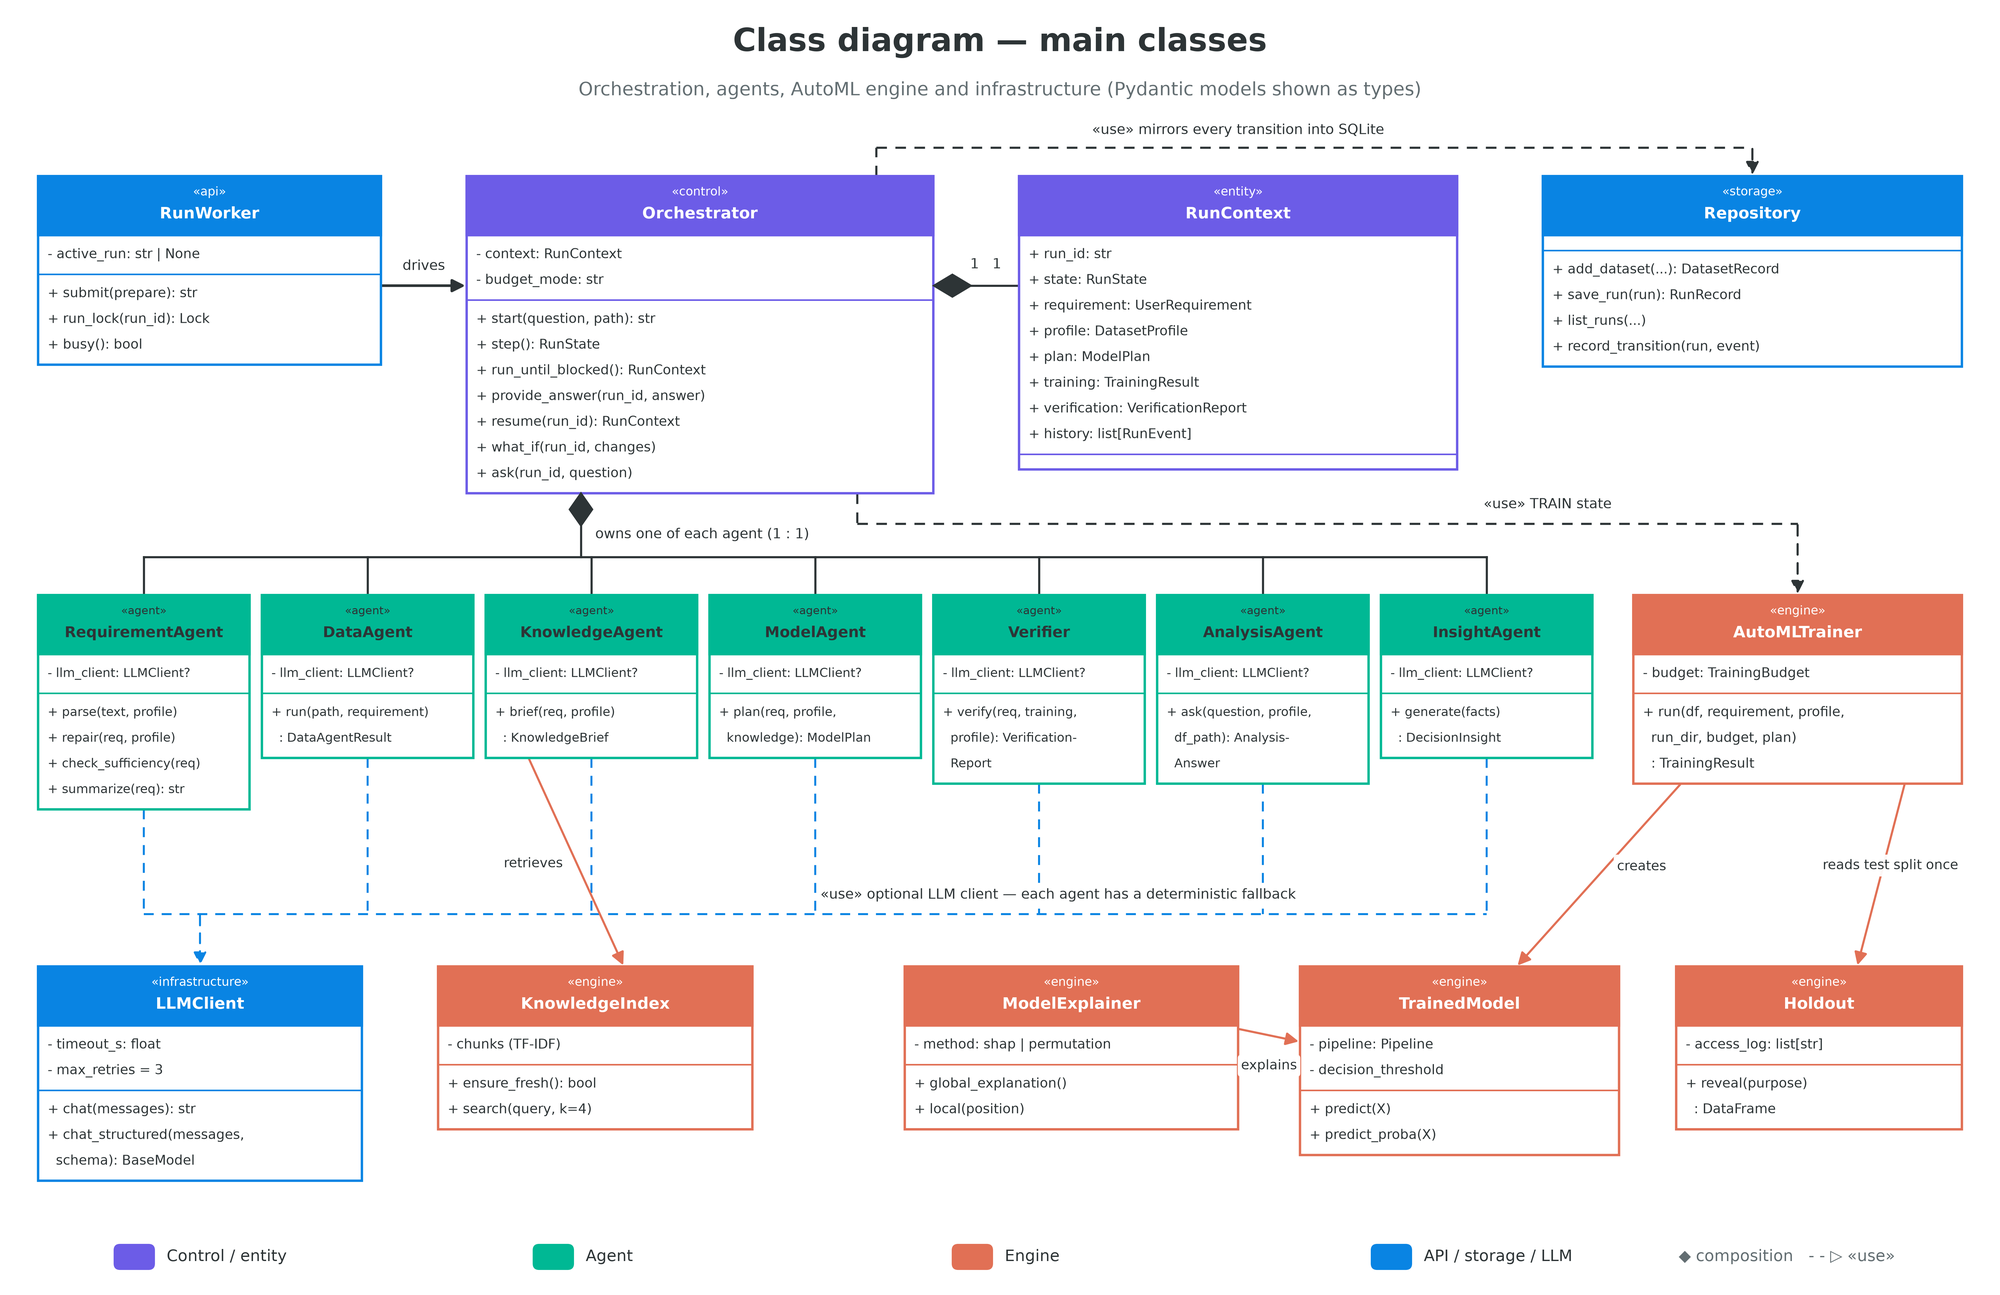
\includegraphics[width=\linewidth,height=7.3in,keepaspectratio]{figures/class_diagram.png}
  \caption{Class diagram of the main classes}\label{fig:4.5}
\end{figure}

\subsection{Sequence Diagram}\label{sec:4.5.3}

The user uploads a CSV; the API saves it, caches its profile and returns the dataset id. The user starts an analysis; the API hands the run to the RunWorker and returns \code{202} at once. The Orchestrator runs the agents, the AutoML engine and the decision steps, saving \code{state.json} and an event after every transition, while the UI polls \code{GET /\allowbreak{}runs/\allowbreak{}\{id\}} every two seconds. Finally the user opens results and reports and runs a what-if with the trained model (Figure~\ref{fig:4.6}).

\begin{figure}[htbp]
  \centering
  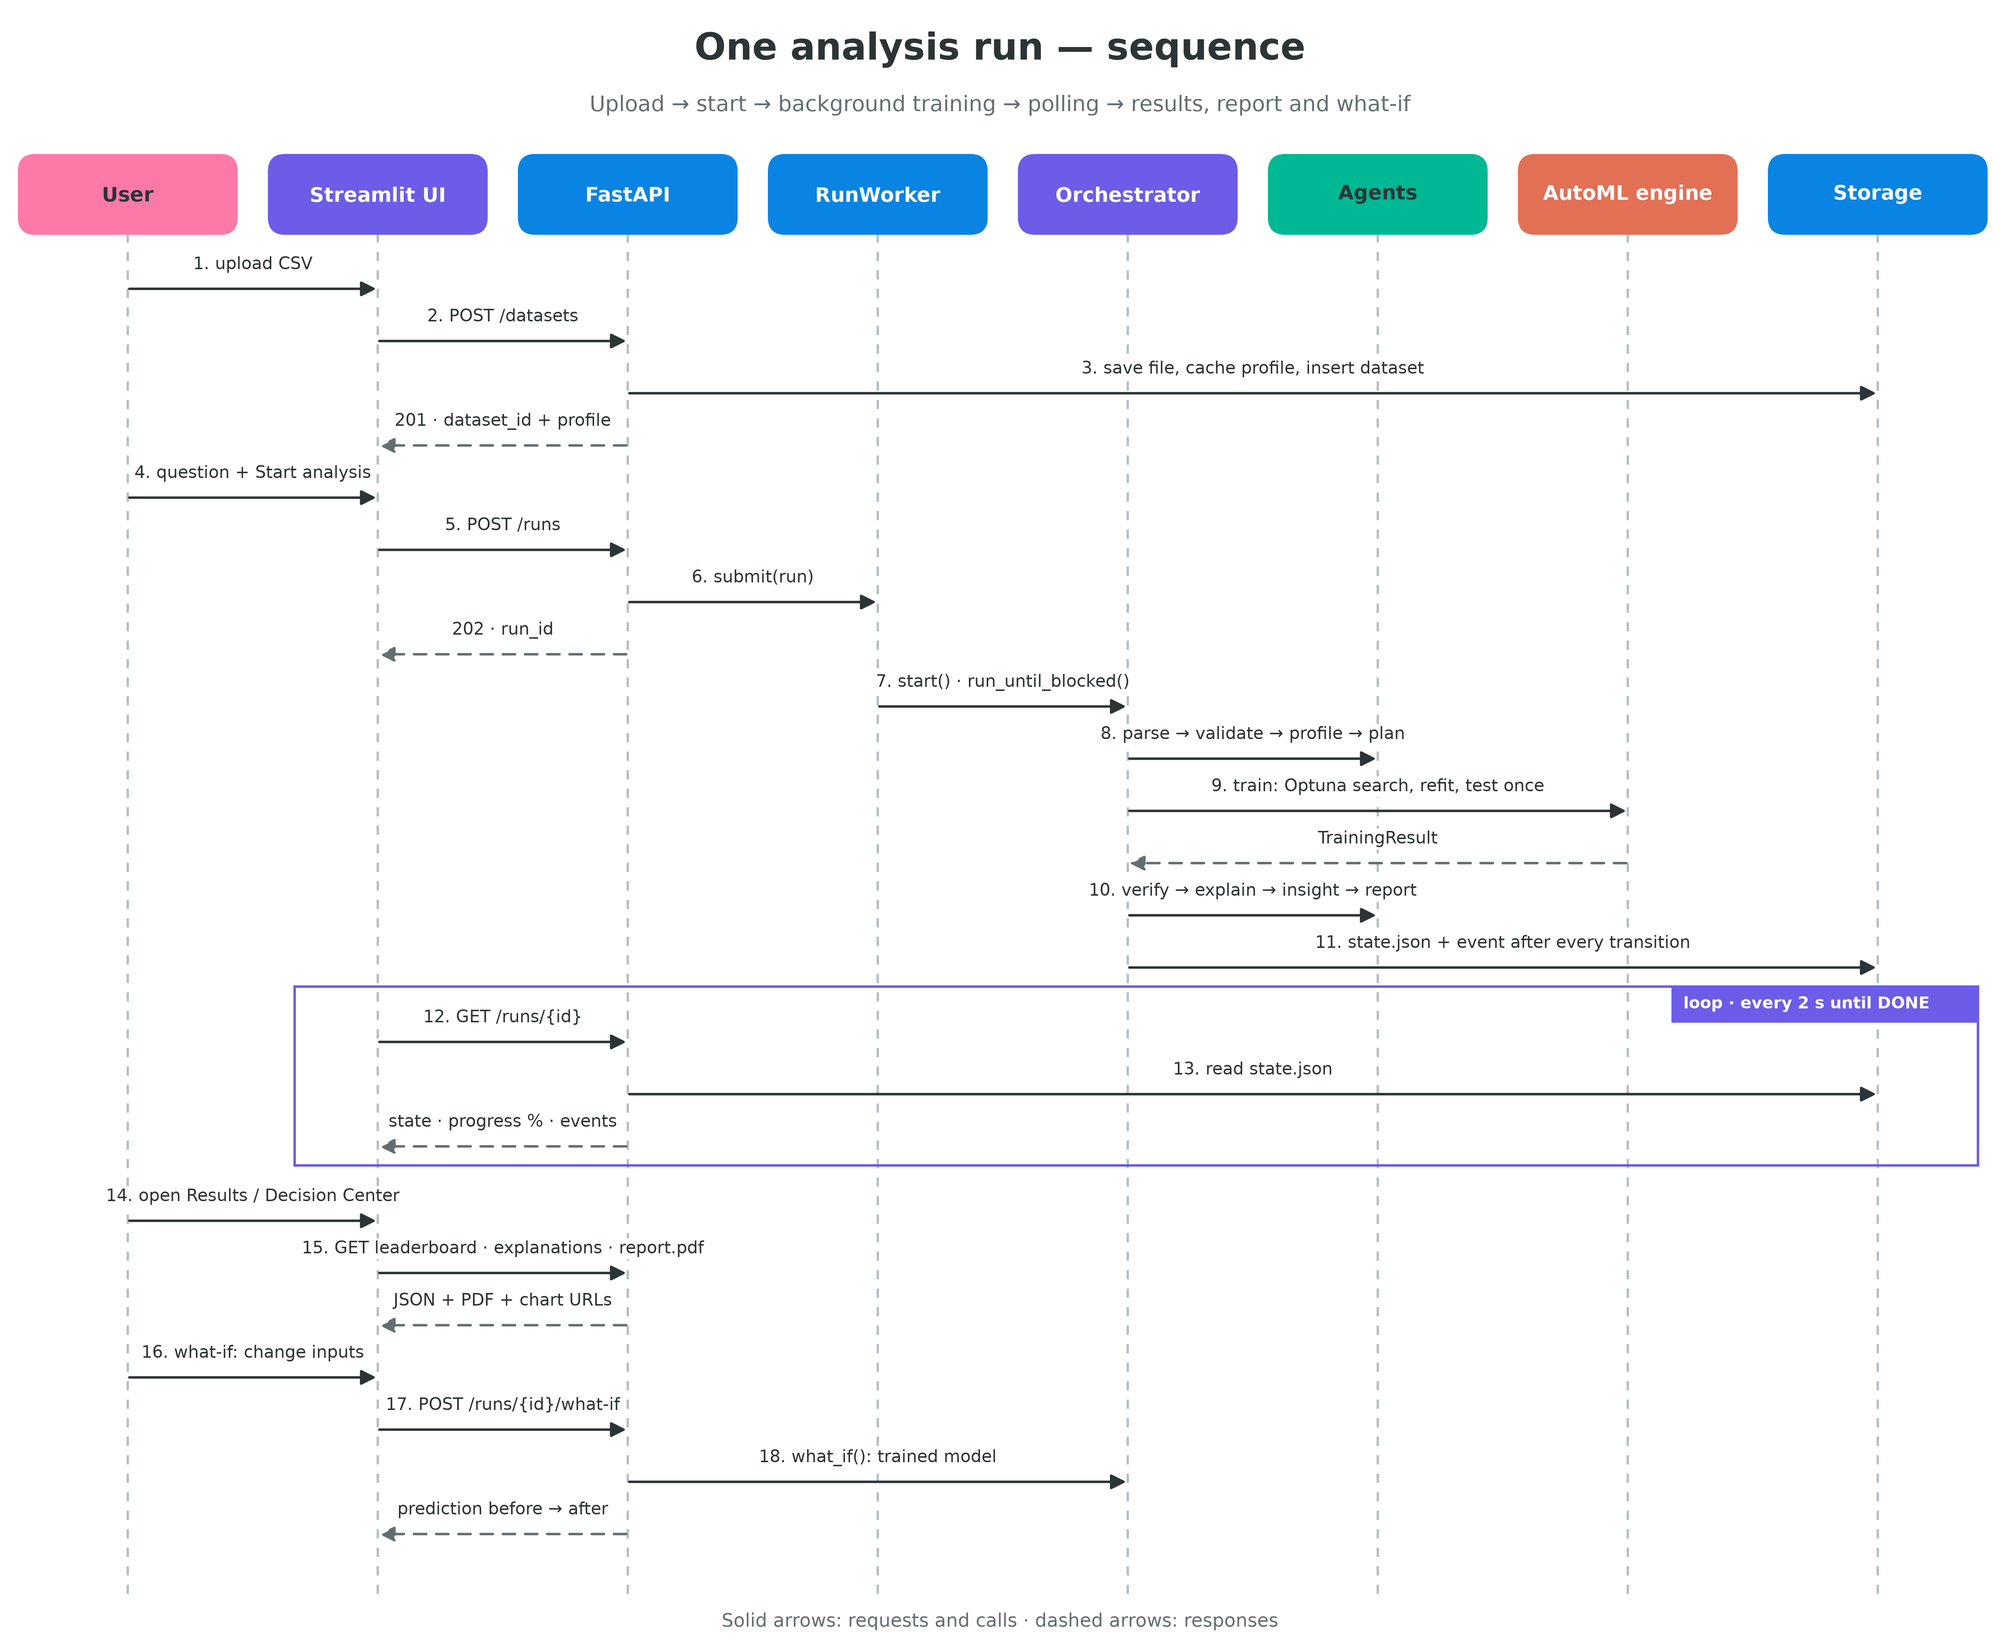
\includegraphics[width=\linewidth,height=7.3in,keepaspectratio]{figures/sequence_one_run.png}
  \caption{Sequence diagram of one analysis run}\label{fig:4.6}
\end{figure}

\subsection{State Chart Diagram}\label{sec:4.5.4}

Each state has one handler that returns the next state. INIT checks relevance (an irrelevant request ends in DONE with a polite reply); PARSE and VALIDATE build and check the requirement, waiting in NEEDS\_INPUT for answers (at most two rounds); PROFILE, PLAN, TRAIN and VERIFY build and check the model; a failed check returns once to PLAN with the full budget, after which the run continues flagged \textit{not verified}; EXPLAIN, INSIGHT and REPORT produce the decision support. Any unhandled error moves the run to FAILED (Figure~\ref{fig:4.7}).

\begin{figure}[htbp]
  \centering
  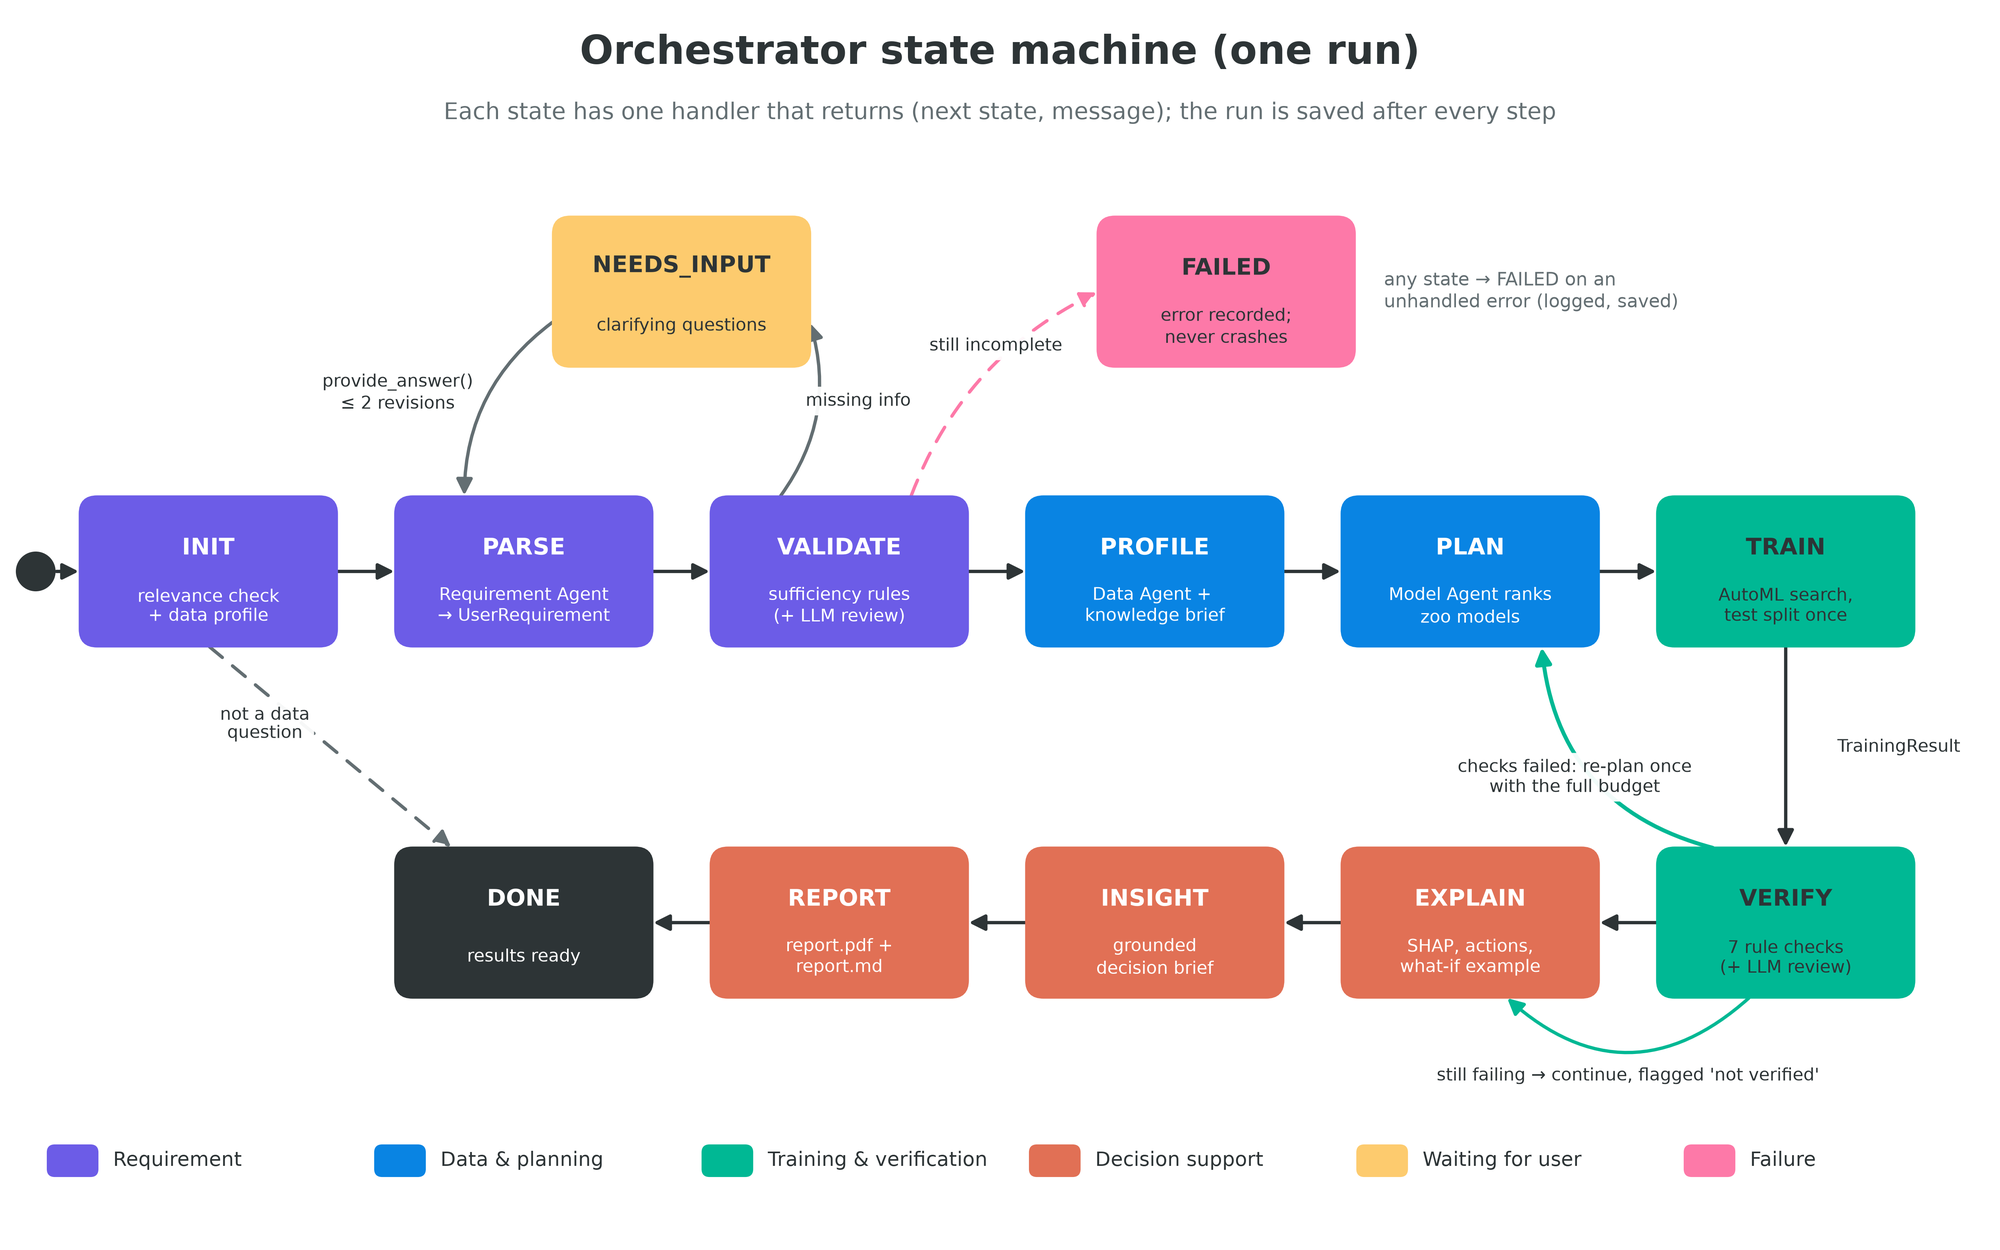
\includegraphics[width=\linewidth,height=7.3in,keepaspectratio]{figures/agent_workflow.png}
  \caption{State chart diagram of a run}\label{fig:4.7}
\end{figure}

\subsection{Activity Diagram}\label{sec:4.5.5}

Figure~\ref{fig:4.8} shows one analysis in four swimlanes --- business user, UI and API, Orchestrator and agents, engines --- with the three decision points of the workflow: is the request relevant, is enough information available, and did verification pass.

\begin{figure}[htbp]
  \centering
  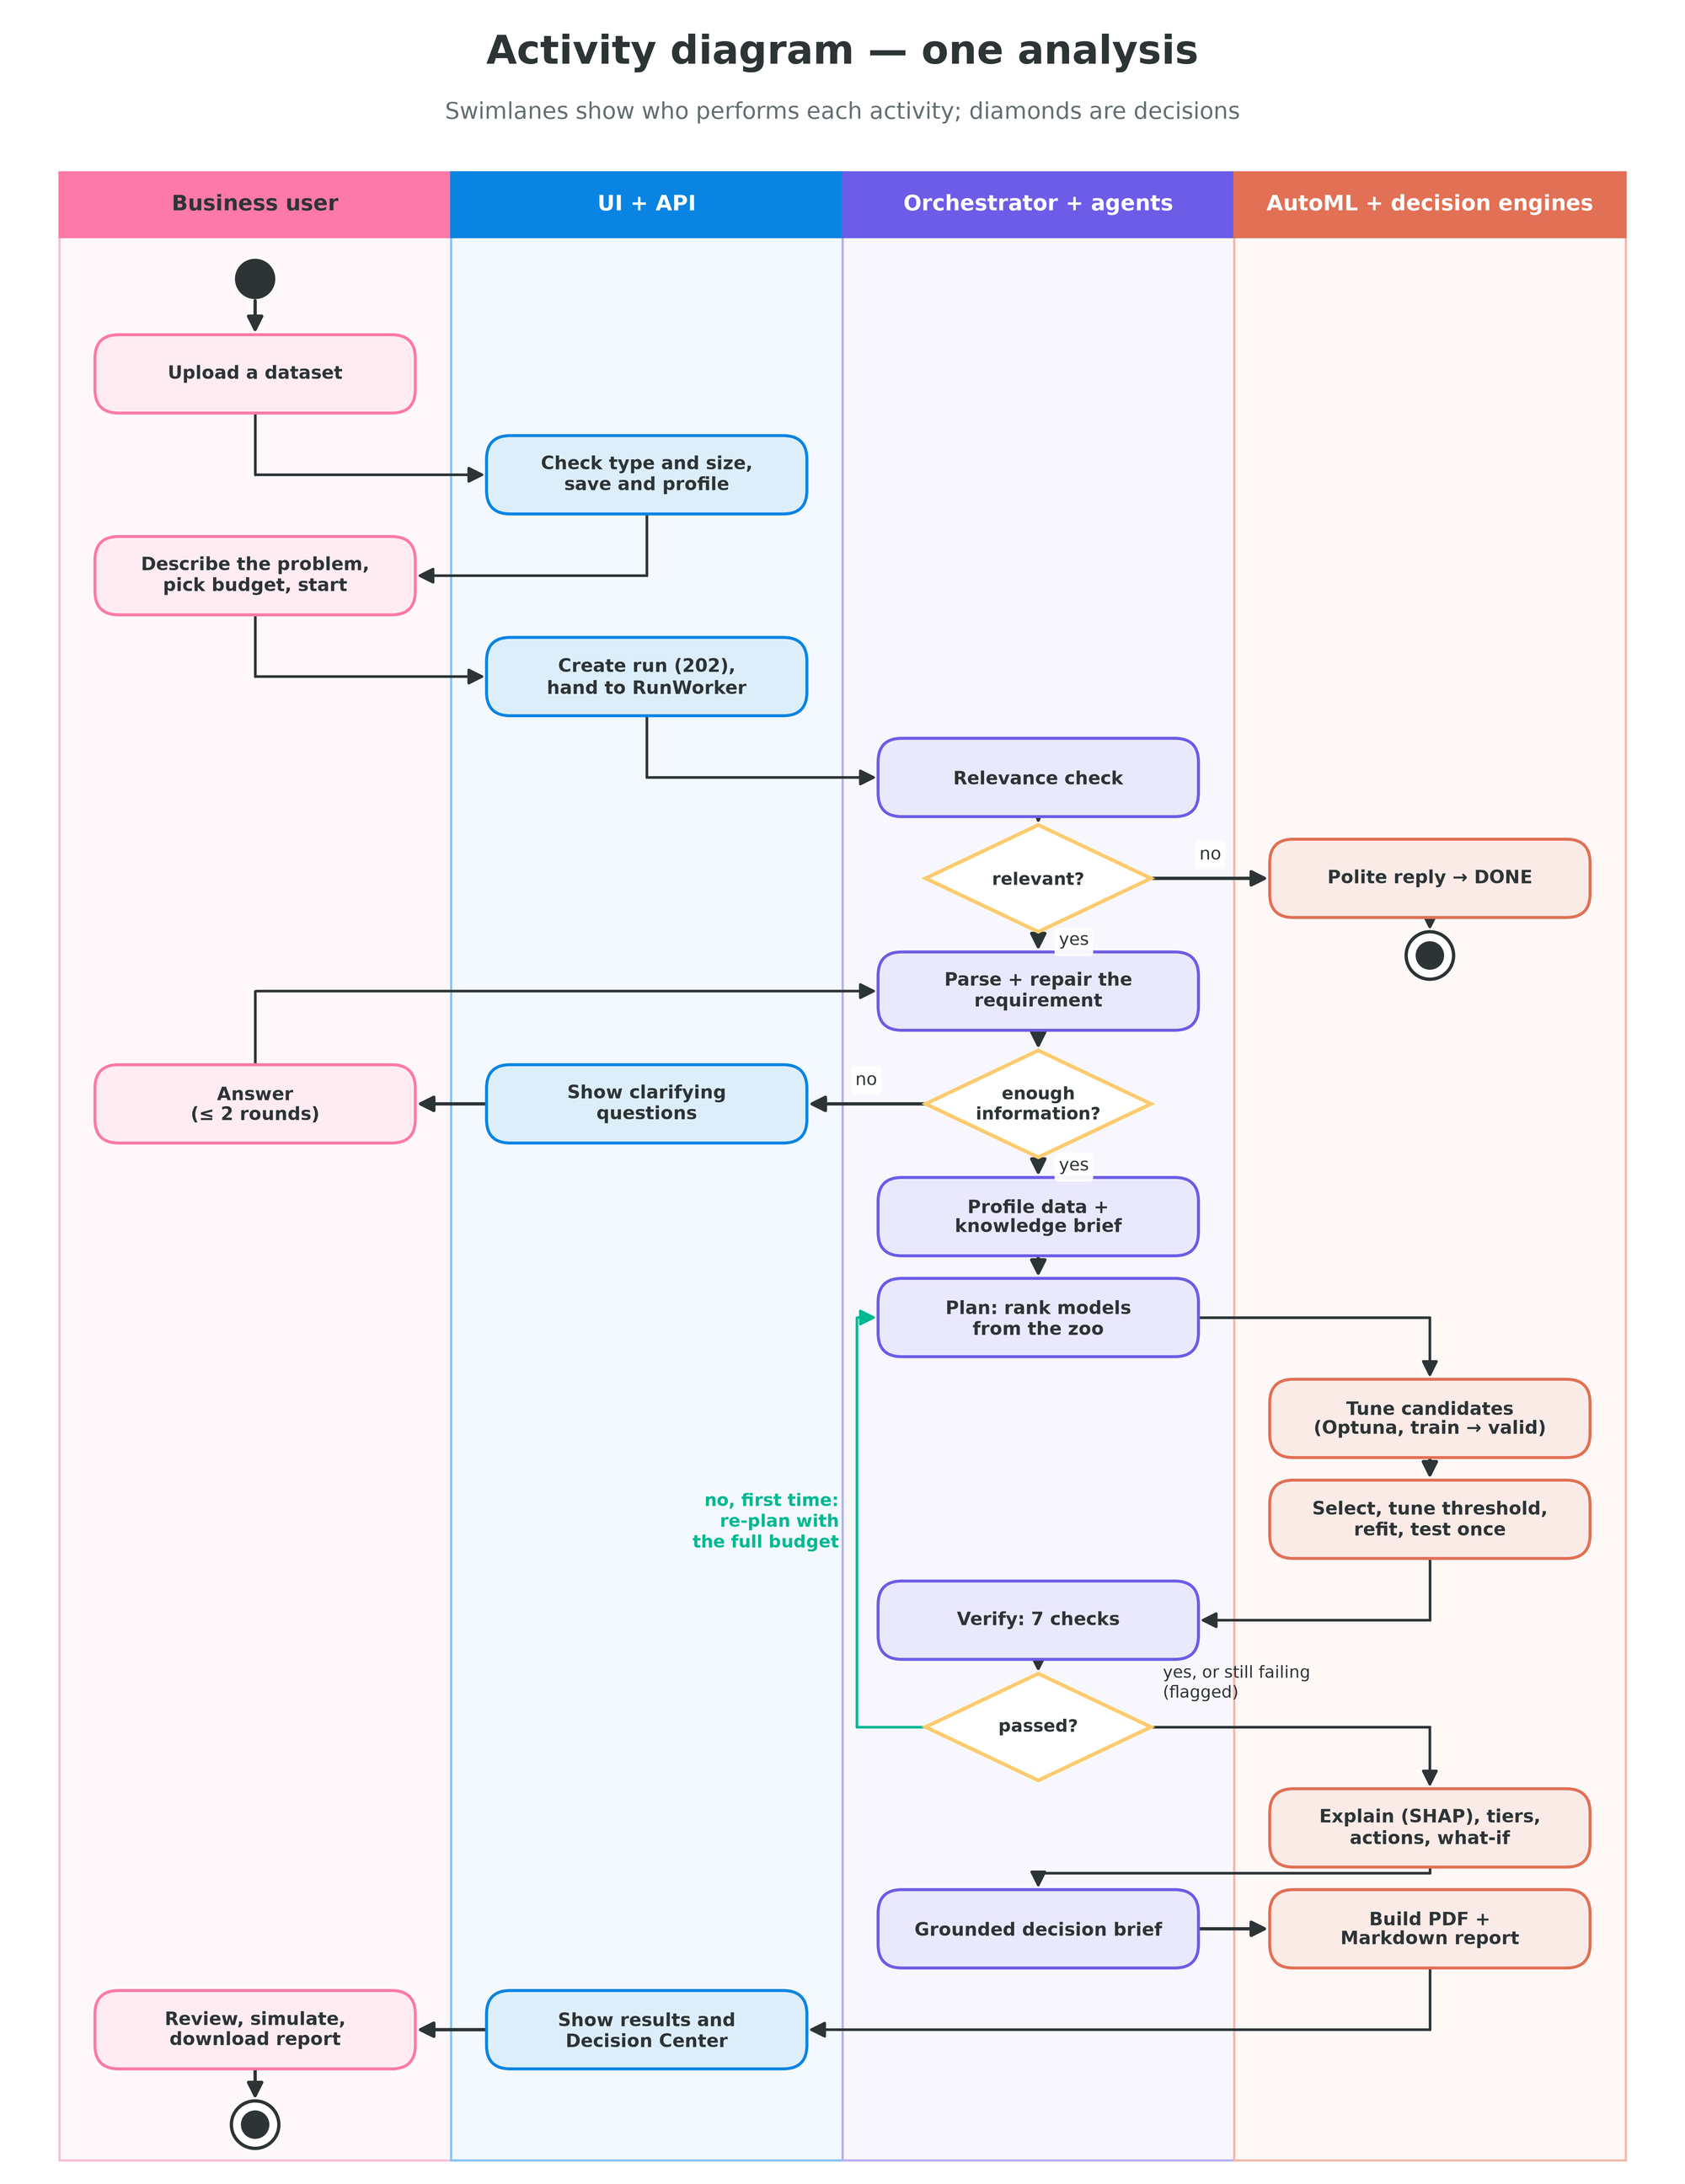
\includegraphics[width=\linewidth,height=7.3in,keepaspectratio]{figures/activity_diagram.png}
  \caption{Activity diagram of one analysis}\label{fig:4.8}
\end{figure}

\subsection{Component and Deployment Diagram}\label{sec:4.5.6}

Everything runs on one Windows PC. The browser shows the dashboard served by the Streamlit process (port 8501), whose pages call the Uvicorn + FastAPI process (port 8000) over \code{127.0.0.1}. Inside the API process, the routes hand work to the RunWorker thread (Orchestrator, agents, engines) and the storage component reads and writes \code{workspace/}. \textit{Ask Your Data} spawns a separate sandbox process. The LLM provider and web search are optional external services, and \code{.env} is read only by the API process (Figure~\ref{fig:4.9}).

\begin{figure}[htbp]
  \centering
  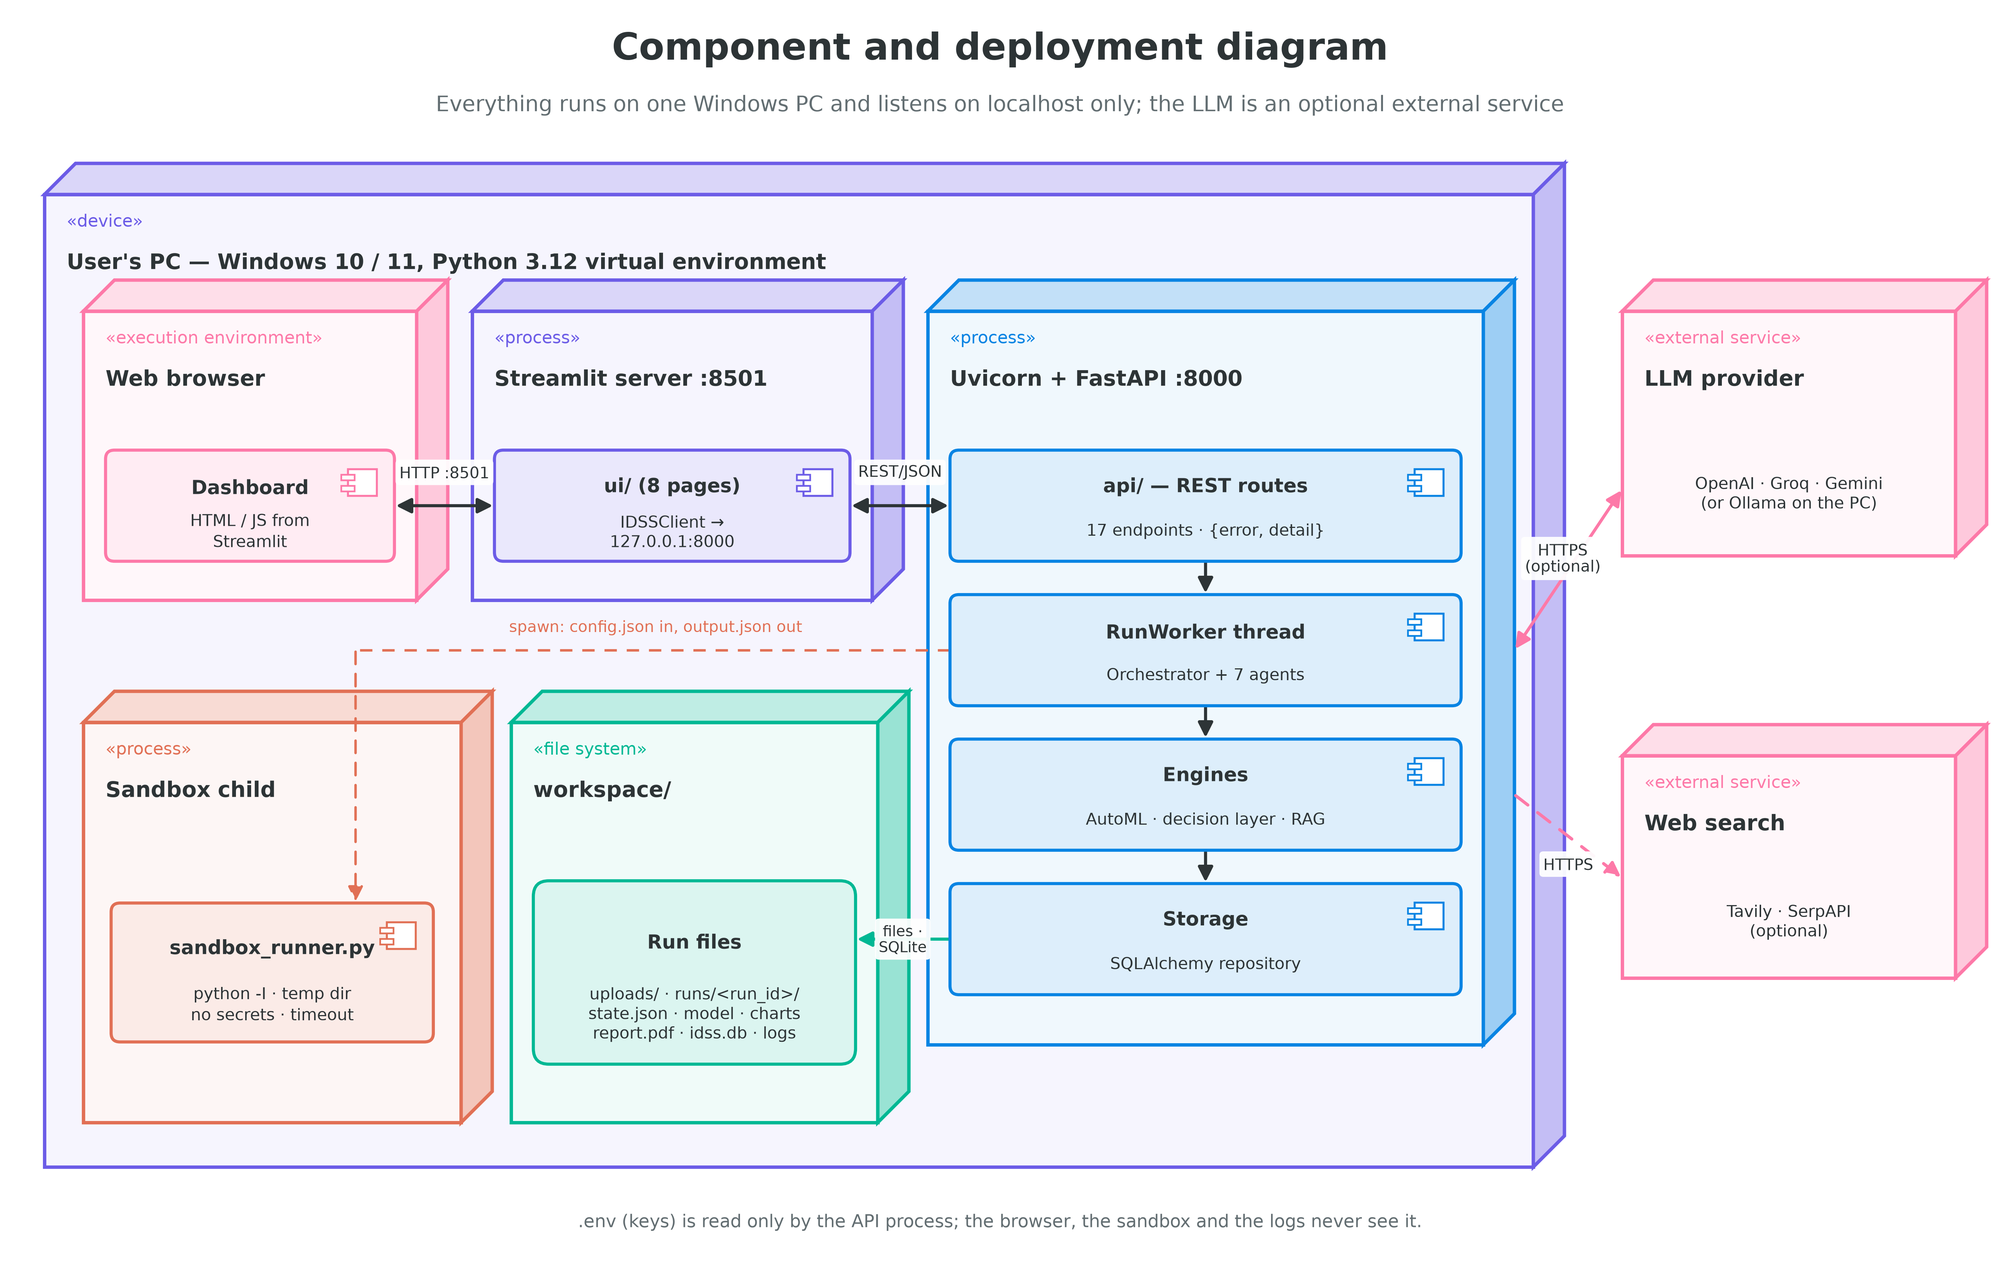
\includegraphics[width=\linewidth,height=7.3in,keepaspectratio]{figures/deployment_diagram.png}
  \caption{Component and deployment diagram}\label{fig:4.9}
\end{figure}

\FloatBarrier
\section{Database Design}\label{sec:4.6}

Each run's \code{state.json} is the source of truth; an SQLite database (\code{workspace/\allowbreak{}idss.db}, write-ahead logging, foreign keys on) indexes datasets, runs and events for fast listing (Figure~\ref{fig:4.10}, Table~\ref{tab:4.7}). A dataset is used by many runs (on delete: set null) and a run has many events (on delete: cascade). The Orchestrator writes the run and its newest event in one transaction after every transition; a database error is only logged.

\begin{figure}[htbp]
  \centering
  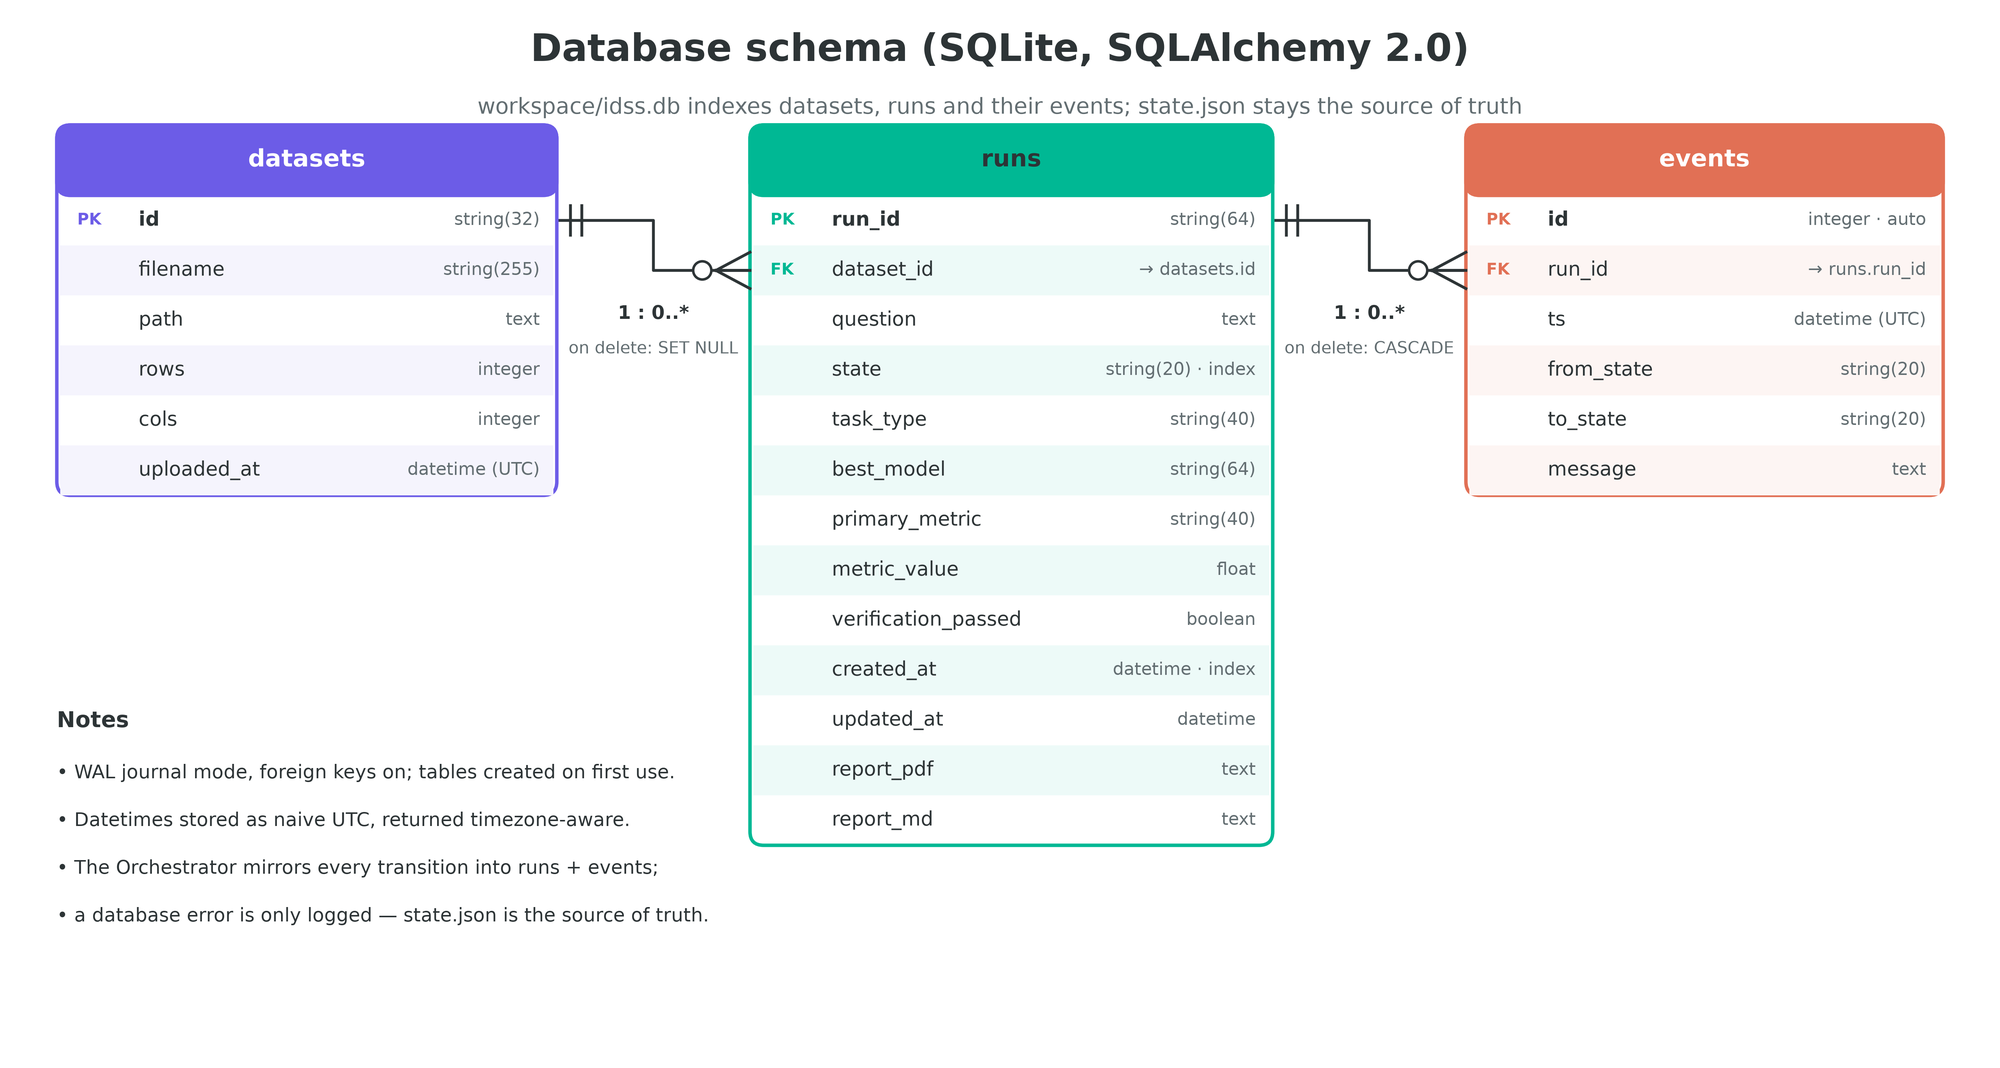
\includegraphics[width=\linewidth,height=7.3in,keepaspectratio]{figures/er_diagram.png}
  \caption{Entity--relationship diagram of the database}\label{fig:4.10}
\end{figure}

\begin{table}[H]
\centering
\linespread{1}\small
\setlength{\tabcolsep}{4pt}
\caption{Database tables}\label{tab:4.7}
\begin{tabular}{|>{\raggedright\arraybackslash\hspace{0pt}}p{\dimexpr 0.1414\linewidth-2\tabcolsep-2\arrayrulewidth\relax}|>{\raggedright\arraybackslash\hspace{0pt}}p{\dimexpr 0.5764\linewidth-2\tabcolsep-2\arrayrulewidth\relax}|>{\raggedright\arraybackslash\hspace{0pt}}p{\dimexpr 0.2821\linewidth-2\tabcolsep-2\arrayrulewidth\relax}|}
\hline
\rowcolor{tableheader}\textbf{Table} & \textbf{Key columns} & \textbf{Purpose} \\
\hline
\code{datasets} & \code{id} (PK), \code{filename}, \code{path}, \code{rows}, \code{cols}, \code{uploaded\_\allowbreak{}at} & One row per uploaded file \\ \hline
\code{runs} & \code{run\_\allowbreak{}id} (PK), \code{dataset\_\allowbreak{}id} (FK), \code{question}, \code{state}, \code{task\_\allowbreak{}type}, \code{best\_\allowbreak{}model}, \code{primary\_\allowbreak{}metric}, \code{metric\_\allowbreak{}value}, \code{verification\_\allowbreak{}passed}, timestamps, report paths & Summary of each run \\ \hline
\code{events} & \code{id} (PK), \code{run\_\allowbreak{}id} (FK), \code{ts}, \code{from\_\allowbreak{}state}, \code{to\_\allowbreak{}state}, \code{message} & One row per state transition \\ \hline
\end{tabular}
\end{table}

\FloatBarrier
\section{Summary}\label{sec:4.7}

This chapter specified twenty functional and thirteen non-functional requirements, the data, hardware and software requirements and an SRS summary, and presented the design: a six-layer architecture, Level 0 and Level 1 data flow diagrams, six UML views and the database schema.

% Generated by scripts/build_latex.py from docs/report/ch5_implementation.md: edit the Markdown, not this file.
\chapter{Coding and Implementation}\label{ch:5}

This chapter describes how the design was implemented: the main algorithms as pseudo-code (Section~\ref{sec:5.1}), the development environment (Section~\ref{sec:5.2}), the modules with their owners (Section~\ref{sec:5.3}), short extracts of the real code (Section~\ref{sec:5.4}) and the user interface (Section~\ref{sec:5.5}).

\FloatBarrier
\section{Algorithms / Steps}\label{sec:5.1}

Names in \code{code font} are the real functions and constants in the repository.

\begin{algorithm}[H]
  \caption{Orchestrator state machine (\code{Orchestrator.step}, \code{run\_\allowbreak{}until\_\allowbreak{}blocked})}\label{alg:5.1}
  \noindent\fcolorbox{codeframe}{codebg}{\begin{minipage}{\dimexpr\linewidth-2\fboxsep-2\fboxrule\relax}
  \linespread{1}\small
  \begin{algorithmic}
    \State \textbf{procedure} RUN\_UNTIL\_BLOCKED(ctx) \Comment{MAX\_STEPS = 50}
    \State \hspace*{1.50em}\textbf{repeat} MAX\_STEPS times
    \State \hspace*{3.00em}\textbf{if} ctx.state \ensuremath{\in} \{DONE, FAILED, NEEDS\_INPUT\} \textbf{then} \textbf{return} ctx
    \State \hspace*{3.00em}STEP(ctx)
    \State \hspace*{1.50em}TRANSITION(ctx, FAILED, ``stopped after MAX\_STEPS steps (possible loop)'')
    \Statex
    \State \textbf{procedure} STEP(ctx)
    \State \hspace*{1.50em}\textbf{try} (next, message) \ensuremath{\leftarrow} HANDLERS[ctx.state](ctx) \Comment{one handler per state}
    \State \hspace*{1.50em}\textbf{catch} error e: record e; next \ensuremath{\leftarrow} FAILED \Comment{never crash the caller}
    \State \hspace*{1.50em}TRANSITION(ctx, next, message)
    \Statex
    \State \textbf{procedure} TRANSITION(ctx, next, message)
    \State \hspace*{1.50em}append event(from, to, message, time) to ctx.history; ctx.state \ensuremath{\leftarrow} next
    \State \hspace*{1.50em}write state.json.tmp, then atomically replace state.json \Comment{\ensuremath{\leq} 3 retries on Windows locks}
    \State \hspace*{1.50em}\textbf{try} record run + event in SQLite (one transaction) \textbf{catch} \ensuremath{\rightarrow} log only
  \end{algorithmic}
  \end{minipage}}
\end{algorithm}

\begin{algorithm}[H]
  \caption{Requirement parsing and repair (\code{RequirementAgent.\allowbreak{}parse}, \code{repair}, \code{check\_\allowbreak{}sufficiency})}\label{alg:5.2}
  \noindent\fcolorbox{codeframe}{codebg}{\begin{minipage}{\dimexpr\linewidth-2\fboxsep-2\fboxrule\relax}
  \linespread{1}\small
  \begin{algorithmic}
    \State R \ensuremath{\leftarrow} LLM structured output for question q and format\_profile(P) \Comment{names, types, \% missing only}
    \State \hspace*{1.50em}(no LLM: R \ensuremath{\leftarrow} requirement\_from\_profile(q, P))
    \State \textbf{if} R.target is not a usable column of P (numeric / categorical / boolean, \textgreater{} 1 value)
    \State \hspace*{1.50em}\textbf{then} note the reason; R.target \ensuremath{\leftarrow} P.suggested\_target
    \State \textbf{if} task type implied by P for R.target \ensuremath{\neq} R.task\_type \textbf{then} note; R.task\_type \ensuremath{\leftarrow} implied type
    \State remove metrics of the wrong family; \textbf{if} none left \textbf{then} R.metrics \ensuremath{\leftarrow} TASK\_METRICS[task]
    \State missing \ensuremath{\leftarrow} rules (goal unclear? no target for a supervised task? confidence \textless{} 0.4?) \ensuremath{\cup} LLM review
    \State \textbf{if} missing \ensuremath{\neq} \ensuremath{\emptyset} \textbf{then} ask \ensuremath{\leq} 3 clarifying questions \ensuremath{\rightarrow} NEEDS\_INPUT (at most 2 rounds per run)
  \end{algorithmic}
  \end{minipage}}
\end{algorithm}

\begin{algorithm}[H]
  \caption{AutoML search, selection and single test evaluation (\code{AutoMLTrainer.run}, \code{tuner.tune})}\label{alg:5.3}
  \noindent\fcolorbox{codeframe}{codebg}{\begin{minipage}{\dimexpr\linewidth-2\fboxsep-2\fboxrule\relax}
  \linespread{1}\small
  \begin{algorithmic}
    \State (train, valid, test) \ensuremath{\leftarrow} SPLIT(D, 70/20/10); wrap test in Holdout; fit preprocessing on train
    \State \textbf{for} each candidate m in the plan (\ensuremath{\leq} budget.max\_candidates) \textbf{do}
    \State \hspace*{1.50em}\textbf{if} total time is used up \textbf{then} mark m ``skipped''; continue
    \State \hspace*{1.50em}study \ensuremath{\leftarrow} Optuna(TPE sampler(seed), median pruner)
    \State \hspace*{1.50em}\textbf{for} each trial (\ensuremath{\leq} n\_trials, \ensuremath{\leq} timeout per model) \textbf{do}
    \State \hspace*{3.00em}\ensuremath{\theta} \ensuremath{\leftarrow} sample(m.search\_space)
    \State \hspace*{3.00em}\textbf{if} \textbar{}train\textbar{} \ensuremath{\geq} 2000 \textbf{then} score on half the rows first; prune \textbf{if} below the median
    \State \hspace*{3.00em}score \ensuremath{\leftarrow} metric(fit(m, \ensuremath{\theta}, train), valid) \Comment{errors \ensuremath{\rightarrow} trial pruned, search continues}
    \State \hspace*{1.50em}refit best \ensuremath{\theta} on train; tune threshold \textbf{if} binary (Algorithm 5.4); record valid score, time, size
    \State mark constraint violations; best \ensuremath{\leftarrow} best valid score without violations
    \State model \ensuremath{\leftarrow} Pipeline(preprocessing, best) refitted on train \ensuremath{\cup} valid
    \State score model and a trivial baseline on Holdout.reveal(``final\_evaluation'') \Comment{the only test read}
  \end{algorithmic}
  \end{minipage}}
\end{algorithm}

\begin{algorithm}[H]
  \caption{Decision-threshold tuning (\code{evaluator.\allowbreak{}tune\_\allowbreak{}threshold})}\label{alg:5.4}
  \noindent\fcolorbox{codeframe}{codebg}{\begin{minipage}{\dimexpr\linewidth-2\fboxsep-2\fboxrule\relax}
  \linespread{1}\small
  \begin{algorithmic}
    \State (t*, s*) \ensuremath{\leftarrow} (0.5, M(y\_valid, p \ensuremath{\geq} 0.5))
    \State \textbf{for} t in 0.05, 0.06, \ldots{}, 0.95 \textbf{do} \Comment{91 cut-offs, validation split only}
    \State \hspace*{1.50em}s \ensuremath{\leftarrow} M(y\_valid, p \ensuremath{\geq} t); \textbf{if} s \textgreater{} s* \textbf{then} (t*, s*) \ensuremath{\leftarrow} (t, s) \Comment{ties keep 0.5}
    \State \textbf{return} t* \Comment{M \ensuremath{\in} \{F1, accuracy, balanced accuracy\}}
  \end{algorithmic}
  \end{minipage}}
\end{algorithm}

\begin{algorithm}[H]
  \caption{Verification and re-planning (\code{Verifier.verify}, \code{Orchestrator.\allowbreak{}\_\allowbreak{}handle\_\allowbreak{}verify})}\label{alg:5.5}
  \noindent\fcolorbox{codeframe}{codebg}{\begin{minipage}{\dimexpr\linewidth-2\fboxsep-2\fboxrule\relax}
  \linespread{1}\small
  \begin{algorithmic}
    \State checks \ensuremath{\leftarrow} metric targets met \ensuremath{\cdot} beats the baseline \ensuremath{\cdot} no constraint violated \ensuremath{\cdot} \ensuremath{\geq} 30 test rows \ensuremath{\cdot}
    \State \hspace*{3.38em}test accesses = [``final\_evaluation''] \ensuremath{\cdot} no leakage warning \ensuremath{\cdot} train \ensuremath{-} test gap \textless{} 0.15
    \State \textbf{if} all pass \textbf{then} next \ensuremath{\leftarrow} EXPLAIN
    \State \textbf{else} \textbf{if} not yet re-planned \textbf{then} next \ensuremath{\leftarrow} PLAN with the full budget and the checks' recommendations
    \State \textbf{else} next \ensuremath{\leftarrow} EXPLAIN, results flagged ``not verified'' \Comment{never FAILED for this reason}
  \end{algorithmic}
  \end{minipage}}
\end{algorithm}

\begin{algorithm}[H]
  \caption{Greedy counterfactual search (\code{recommender.\allowbreak{}counterfactual})}\label{alg:5.6}
  \noindent\fcolorbox{codeframe}{codebg}{\begin{minipage}{\dimexpr\linewidth-2\fboxsep-2\fboxrule\relax}
  \linespread{1}\small
  \begin{algorithmic}
    \State p \ensuremath{\leftarrow} f(x); \ensuremath{\Delta} \ensuremath{\leftarrow} []
    \State \textbf{repeat} at most 3 times \textbf{while} p \ensuremath{\geq} t
    \State \hspace*{1.50em}\textbf{try} every (column a \ensuremath{\in} actionable \ensuremath{\setminus} \ensuremath{\Delta}, observed value v \ensuremath{\neq} x[a]) in one batch
    \State \hspace*{1.50em}take the option with the lowest probability p\ensuremath{{}'}; stop \textbf{if} p\ensuremath{{}'} \ensuremath{\geq} p
    \State \hspace*{1.50em}x[a] \ensuremath{\leftarrow} v; \ensuremath{\Delta} \ensuremath{\leftarrow} \ensuremath{\Delta} \ensuremath{\cup} \{a\}; p \ensuremath{\leftarrow} p\ensuremath{{}'}
    \State \textbf{if} p \textless{} t \textbf{then} undo every change in \ensuremath{\Delta} that is not needed to stay below t \Comment{minimal set}
    \State \textbf{return} \ensuremath{\Delta}, probability before and after, success = (p \textless{} t)
  \end{algorithmic}
  \end{minipage}}
\end{algorithm}

\begin{algorithm}[H]
  \caption{Grounded insight generation (\code{InsightAgent.\allowbreak{}generate}, \code{unsupported\_\allowbreak{}numbers})}\label{alg:5.7}
  \noindent\fcolorbox{codeframe}{codebg}{\begin{minipage}{\dimexpr\linewidth-2\fboxsep-2\fboxrule\relax}
  \linespread{1}\small
  \begin{algorithmic}
    \State \textbf{if} no LLM \textbf{then} \textbf{return} TEMPLATE(facts) \Comment{complete and itself grounded}
    \State allowed \ensuremath{\leftarrow} every number in the facts (also inside strings)
    \State \textbf{for} attempt = 1, 2 \textbf{do}
    \State \hspace*{1.50em}draft \ensuremath{\leftarrow} LLM(facts, feedback)
    \State \hspace*{1.50em}bad \ensuremath{\leftarrow} numbers in draft not in \{0..10, 100\} and not matching a fact (\ensuremath{\pm}1\%, rounding, \ensuremath{\times}100 for \%)
    \State \hspace*{1.50em}\textbf{if} bad = \ensuremath{\emptyset} \textbf{then} \textbf{return} draft
    \State \hspace*{1.50em}feedback \ensuremath{\leftarrow} ``numbers not in the facts: '' + bad
    \State \textbf{return} TEMPLATE(facts) with the failed grounding result
  \end{algorithmic}
  \end{minipage}}
\end{algorithm}

\begin{algorithm}[H]
  \caption{Sandboxed execution of LLM-written code (\code{sandbox.check\_\allowbreak{}code}, \code{run\_\allowbreak{}code})}\label{alg:5.8}
  \noindent\fcolorbox{codeframe}{codebg}{\begin{minipage}{\dimexpr\linewidth-2\fboxsep-2\fboxrule\relax}
  \linespread{1}\small
  \begin{algorithmic}
    \State reject code \textgreater{} 20 000 characters or with a syntax error
    \State \textbf{for} each AST node: import outside \{pandas, numpy, math, statistics, datetime, json, re\},
    \State \hspace*{1.50em}blocked name (open, eval, exec, \_\_import\_\_, getattr, os, sys, \ldots{}), private attribute,
    \State \hspace*{1.50em}I/O attribute (read\_*, to\_csv, \ldots{}) or other blocked attribute (query, load, \ldots{}) \ensuremath{\rightarrow} problem
    \State \textbf{if} problems \textbf{then} \textbf{return} ``Blocked by the sandbox'' (nothing runs)
    \State run ``python -I sandbox\_runner.py'' in a temporary folder with restricted built-ins,
    \State \hspace*{1.50em}a guarded \_\_import\_\_ and an environment without secrets; kill after the timeout (20 s)
    \State \textbf{return} stdout (\ensuremath{\leq} 20 KB) and result (\ensuremath{\leq} 200 rows)
  \end{algorithmic}
  \end{minipage}}
\end{algorithm}

\FloatBarrier
\section{Software and Hardware for Development}\label{sec:5.2}

The runtime libraries are those of Table~\ref{tab:4.5}. Table~\ref{tab:5.1} lists the additional development tools and Table~\ref{tab:5.2} the hardware.

\begin{table}[H]
\centering
\linespread{1}\small
\setlength{\tabcolsep}{4pt}
\caption{Development tools}\label{tab:5.1}
\begin{tabular}{|>{\raggedright\arraybackslash\hspace{0pt}}p{\dimexpr 0.2675\linewidth-2\tabcolsep-2\arrayrulewidth\relax}|>{\raggedright\arraybackslash\hspace{0pt}}p{\dimexpr 0.2254\linewidth-2\tabcolsep-2\arrayrulewidth\relax}|>{\raggedright\arraybackslash\hspace{0pt}}p{\dimexpr 0.5071\linewidth-2\tabcolsep-2\arrayrulewidth\relax}|}
\hline
\rowcolor{tableheader}\textbf{Tool} & \textbf{Version} & \textbf{Use} \\
\hline
Python \code{venv} + pip & Python 3.12.0 & Isolated environment with pinned dependencies (\code{requirements.txt}) \\ \hline
pytest, pytest-cov, httpx2 & 9.1.1, 7.1.0, 2.13.1 & Automated tests, coverage, API test client \\ \hline
ruff & 0.16.10 & Linting \\ \hline
Playwright (Chromium) & 1.63.0 & Automated UI screenshots \\ \hline
Git & --- & Version control, one commit per increment \\ \hline
PowerShell & Windows PowerShell & Start scripts (\code{run\_\allowbreak{}api.ps1}, \code{run\_\allowbreak{}ui.ps1}, \code{run\_\allowbreak{}all.ps1}) \\ \hline
Claude Code & --- & AI coding assistant for code generation and refactoring \\ \hline
\end{tabular}
\end{table}

An AI coding assistant (Claude Code) was used to help generate and refactor code; all design decisions, integration, testing and evaluation were carried out and verified by the team.

\begin{table}[H]
\centering
\linespread{1}\small
\setlength{\tabcolsep}{4pt}
\caption{Development hardware}\label{tab:5.2}
\begin{tabular}{|>{\raggedright\arraybackslash\hspace{0pt}}p{\dimexpr 0.2571\linewidth-2\tabcolsep-2\arrayrulewidth\relax}|>{\raggedright\arraybackslash\hspace{0pt}}p{\dimexpr 0.7429\linewidth-2\tabcolsep-2\arrayrulewidth\relax}|}
\hline
\rowcolor{tableheader}\textbf{Item} & \textbf{Specification} \\
\hline
Development machine & ASUS TUF Gaming F15 (FX506HE) laptop, used for development, testing, the evaluation and this report \\ \hline
Processor & 11th Gen Intel Core i7-11800H, 2.30 GHz, 8 cores / 16 logical processors \\ \hline
Memory & 16 GB RAM \\ \hline
Storage & 1 TB NVMe SSD (WD PC SN560) \\ \hline
GPU & NVIDIA GeForce RTX 3050 Ti Laptop GPU (4 GB) --- not used by IDSS, which trains on the CPU \\ \hline
Operating system & Windows 11 Home Single Language, 64-bit \\ \hline
Network & Only for package installation and optional LLM calls \\ \hline
\end{tabular}
\end{table}

The evaluation of Chapter~\ref{ch:7} ran on this machine (\code{scripts/\allowbreak{}evaluate.\allowbreak{}py} records Windows 11 and 16 logical CPUs). The minimum hardware for running IDSS is given in Table~\ref{tab:4.4}.

\FloatBarrier
\section{Modules in Project}\label{sec:5.3}

\begingroup
\linespread{1}\small
\setlength{\tabcolsep}{4pt}
\begin{longtable}{|>{\raggedright\arraybackslash\hspace{0pt}}p{\dimexpr 0.0733\linewidth-2\tabcolsep-2\arrayrulewidth\relax}|>{\raggedright\arraybackslash\hspace{0pt}}p{\dimexpr 0.2628\linewidth-2\tabcolsep-2\arrayrulewidth\relax}|>{\raggedright\arraybackslash\hspace{0pt}}p{\dimexpr 0.3935\linewidth-2\tabcolsep-2\arrayrulewidth\relax}|>{\raggedright\arraybackslash\hspace{0pt}}p{\dimexpr 0.2704\linewidth-2\tabcolsep-2\arrayrulewidth\relax}|}
\caption{Modules and responsibilities}\label{tab:5.3}\\
\hline
\rowcolor{tableheader}\textbf{No.} & \textbf{Module} & \textbf{Main files} & \textbf{Member responsible} \\
\hline
\endfirsthead
\hline
\rowcolor{tableheader}\textbf{No.} & \textbf{Module} & \textbf{Main files} & \textbf{Member responsible} \\
\endhead
1 & Foundation & \code{configs/\allowbreak{}settings.\allowbreak{}py}, \code{idss/\allowbreak{}core/} & Raj Vishwas Patil, Chaitany Rajesh Naval \\ \hline
2 & Data module & \code{idss/\allowbreak{}ml/\allowbreak{}data\_\allowbreak{}loader.\allowbreak{}py}, \code{profiler.py}, \code{preprocess.py}, \code{agents/\allowbreak{}data\_\allowbreak{}agent.\allowbreak{}py} & Bhavesh Vinod Patil \\ \hline
3 & Requirement Agent and Orchestrator & \code{agents/\allowbreak{}requirement\_\allowbreak{}agent.\allowbreak{}py}, \code{agents/\allowbreak{}manager.py} & Raj Vishwas Patil, Chaitany Rajesh Naval \\ \hline
4 & AutoML engine and Model Agent & \code{idss/\allowbreak{}ml/\allowbreak{}model\_\allowbreak{}zoo.\allowbreak{}py}, \code{tuner.py}, \code{evaluator.py}, \code{trainer.py}, \code{agents/\allowbreak{}model\_\allowbreak{}agent.\allowbreak{}py} & Bhavesh Vinod Patil, Raj Vishwas Patil \\ \hline
5 & Knowledge base & \code{idss/\allowbreak{}knowledge/}, \code{data/\allowbreak{}knowledge/}, \code{agents/\allowbreak{}knowledge\_\allowbreak{}agent.\allowbreak{}py} & Raj Vishwas Patil \\ \hline
6 & Verifier & \code{agents/\allowbreak{}verifier.py} & Bhavesh Vinod Patil \\ \hline
7 & Sandbox and Analysis Agent & \code{idss/\allowbreak{}execution/}, \code{agents/\allowbreak{}analysis\_\allowbreak{}agent.\allowbreak{}py} & Chaitany Rajesh Naval \\ \hline
8 & Decision layer & \code{idss/\allowbreak{}ml/\allowbreak{}explain.py}, \code{idss/\allowbreak{}decision/\allowbreak{}what\_\allowbreak{}if.\allowbreak{}py}, \code{recommender.py} & Bhavesh Vinod Patil \\ \hline
9 & Insight Agent and reports & \code{agents/\allowbreak{}insight\_\allowbreak{}agent.\allowbreak{}py}, \code{idss/\allowbreak{}decision/\allowbreak{}report\_\allowbreak{}builder.\allowbreak{}py} & Raj Vishwas Patil, Varun Darshan Patil \\ \hline
10 & Storage and REST API & \code{idss/\allowbreak{}storage/}, \code{api/} & Chaitany Rajesh Naval \\ \hline
11 & Streamlit UI & \code{ui/} & Varun Darshan Patil \\ \hline
12 & Evaluation and tooling & \code{scripts/} & Bhavesh Vinod Patil, Varun Darshan Patil \\ \hline
\end{longtable}
\endgroup

The member column follows the roles of Table~\ref{tab:3.4} and the planned allocation of Table~\ref{tab:3.5}; testing, review and integration of every module were shared by the whole team.

\textbf{1. Foundation.} Typed settings from \code{.env} (keys as secret strings, never logged); one logger (loguru, rotating at 10 MB); the only LLM client --- OpenAI-compatible, 60 s default timeout, at most 3 retries with exponential backoff, and \code{chat\_\allowbreak{}structured()}, which validates replies against a Pydantic model and feeds errors back for a retry; the shared Pydantic schemas; and eleven prompt templates with \code{\#\# system} / \code{\#\# user} sections.

\textbf{2. Data module.} Loads CSV (delimiter and encoding detection), Excel, JSON / JSON lines and Parquet; profiles semantic types (numeric, categorical, boolean, datetime, id, text), missing values, the suggested target and task, and warns about leakage (correlation with the target \ensuremath{\geq} 0.98) and imbalance; cleans the data, splits it 70/20/10 and fits a preprocessor (imputation, scaling, one-hot encoding capped at 20 categories). The Data Agent asks the LLM only for a summary of aggregates. \textit{Output:} profile, Parquet splits and \code{preprocessor.\allowbreak{}joblib}.

\textbf{3. Requirement Agent and Orchestrator.} Relevance, parsing, repair and clarifying questions (Algorithm~\ref{alg:5.2}), and the 13-state \code{RunState} machine (Algorithm~\ref{alg:5.1}) with \code{start}, \code{step}, \code{run\_\allowbreak{}until\_\allowbreak{}blocked}, \code{provide\_\allowbreak{}answer}, \code{resume}, \code{abort}, \code{ask} and \code{what\_\allowbreak{}if}. \textit{Output:} \code{RunContext} in \code{workspace/\allowbreak{}runs/\allowbreak{}\textless{}run\_\allowbreak{}id\textgreater{}/\allowbreak{}state.\allowbreak{}json}, mirrored to SQLite.

\textbf{4. AutoML engine and Model Agent.} The model zoo (Table~\ref{tab:5.4}) is the only source of trainable models; each candidate has a \code{build()} function and an Optuna search space, and class weighting switches on when the minority class is below 20\%. Time-series features use only earlier rows. The evaluator holds 19 metrics with their family and direction and measures training time, inference time per row and model size. The Model Agent lets the LLM rank zoo names only (unknown names dropped, requested models first, defaults filling the rest) and parses constraints such as ``inference under 5 ms'' into the plan. Budgets: \textit{fast} 3 models \ensuremath{\times} 15 trials (60 s each, 180 s total); \textit{full} 6 \ensuremath{\times} 40 (180 s each, 1,080 s total). \textit{Output:} \code{TrainingResult}, \code{best\_\allowbreak{}model.joblib}, leaderboard, metrics and test predictions.

\begin{table}[H]
\centering
\linespread{1}\small
\setlength{\tabcolsep}{4pt}
\caption{Model zoo and baselines}\label{tab:5.4}
\begin{tabular}{|>{\raggedright\arraybackslash\hspace{0pt}}p{\dimexpr 0.2698\linewidth-2\tabcolsep-2\arrayrulewidth\relax}|>{\raggedright\arraybackslash\hspace{0pt}}p{\dimexpr 0.5046\linewidth-2\tabcolsep-2\arrayrulewidth\relax}|>{\raggedright\arraybackslash\hspace{0pt}}p{\dimexpr 0.2256\linewidth-2\tabcolsep-2\arrayrulewidth\relax}|}
\hline
\rowcolor{tableheader}\textbf{Task} & \textbf{Candidate models} & \textbf{Baseline (test split)} \\
\hline
Classification & logistic regression, random forest, extra trees, XGBoost, LightGBM, histogram gradient boosting & Majority class \\ \hline
Regression & ridge, random forest, extra trees, XGBoost, LightGBM, histogram gradient boosting & Mean of the target \\ \hline
Time-series forecasting & LightGBM, XGBoost, ridge on lag / rolling / calendar features & Seasonal naive \\ \hline
Clustering & k-means, Gaussian mixture (several EM starts), agglomerative & Random assignment \\ \hline
\end{tabular}
\end{table}

\textbf{5. Knowledge base.} Ten notes in \code{data/\allowbreak{}knowledge/} (churn retention, class imbalance, clustering, explainability, feature leakage, model selection by data size, pricing and demand, regression, tabular classification, time series) are chunked (\ensuremath{\approx} 500 characters, 80 overlap), indexed with TF-IDF, cached and rebuilt when their content changes; retrieval returns 4 passages, at most 2 per note, which the Knowledge Agent condenses into a brief.

\textbf{6. Verifier.} Seven independent checks (Algorithm~\ref{alg:5.5}) with a fixed recommendation for each failure; an optional LLM review adds concerns but never changes the pass / fail decision.

\textbf{7. Sandbox and Analysis Agent.} The static guard and child-process runner of Algorithm~\ref{alg:5.8}; the Analysis Agent sends only column names and types to the LLM and asks it to repair failing code once.

\textbf{8. Decision layer.} \code{ModelExplainer} uses SHAP (tree or linear explainer, \ensuremath{\leq} 500 training rows) or permutation importance and maps values back to original columns; it also builds cluster profiles and a recursive forecast with a \ensuremath{\pm}1.96 \ensuremath{\times} validation-RMSE band. \code{what\_\allowbreak{}if.py} simulates records and segments with validated changes (value, set, add, pct) and structured filters, never evaluated strings. \code{recommender.py} infers actionable columns, builds risk tiers (High \ensuremath{\geq} max(threshold, 70th percentile), Medium \ensuremath{\geq} threshold, Low below), runs counterfactuals (Algorithm~\ref{alg:5.6}) on the 20 riskiest records and computes \ensuremath{\pm}10\% lever effects for regression; every recommendation carries its evidence.

\textbf{9. Insight Agent and reports.} \code{build\_\allowbreak{}facts()} is the only LLM input; the grounding check (Algorithm~\ref{alg:5.7}) guards the brief, with \code{template\_\allowbreak{}insight()} as fallback. \code{report\_\allowbreak{}builder.py} renders one block list as \code{report.pdf} (reportlab) and \code{report.md}.

\textbf{10. Storage and REST API.} SQLAlchemy models and a repository over SQLite; a FastAPI application with 17 endpoints (Table~\ref{tab:5.5}), errors as \code{\{error, detail\}}, \code{409 not\_\allowbreak{}ready} for results not yet computed, and one background RunWorker that answers \code{409 busy} to a second training request. Runs left unfinished by a previous process are marked FAILED at start-up.

\begingroup
\linespread{1}\small
\setlength{\tabcolsep}{4pt}
\begin{longtable}{|>{\raggedright\arraybackslash\hspace{0pt}}p{\dimexpr 0.1280\linewidth-2\tabcolsep-2\arrayrulewidth\relax}|>{\raggedright\arraybackslash\hspace{0pt}}p{\dimexpr 0.4590\linewidth-2\tabcolsep-2\arrayrulewidth\relax}|>{\raggedright\arraybackslash\hspace{0pt}}p{\dimexpr 0.4130\linewidth-2\tabcolsep-2\arrayrulewidth\relax}|}
\caption{REST API endpoints}\label{tab:5.5}\\
\hline
\rowcolor{tableheader}\textbf{Method} & \textbf{Path} & \textbf{Purpose} \\
\hline
\endfirsthead
\hline
\rowcolor{tableheader}\textbf{Method} & \textbf{Path} & \textbf{Purpose} \\
\endhead
GET & \code{/health} & Status, LLM configured (yes / no), version \\ \hline
POST, GET & \code{/datasets} & Upload a file (\ensuremath{\leq} 50 MB) with its profile; list datasets \\ \hline
GET & \code{/datasets/\allowbreak{}\{id\}/\allowbreak{}profile} & Profile of one dataset \\ \hline
POST, GET & \code{/runs} & Start a run (\code{202} + run id); list runs \\ \hline
GET & \code{/runs/\allowbreak{}\{id\}} & State, progress, events, metrics, verification, questions \\ \hline
POST & \code{/runs/\allowbreak{}\{id\}/\allowbreak{}answer} & Answer clarifying questions \\ \hline
GET & \code{/runs/\allowbreak{}\{id\}/\allowbreak{}leaderboard}, \code{/explanations}, \code{/recommendations}, \code{/insight} & Results of a finished run \\ \hline
POST & \code{/runs/\allowbreak{}\{id\}/\allowbreak{}what-if} & Record or segment simulation \\ \hline
POST & \code{/runs/\allowbreak{}\{id\}/\allowbreak{}ask} & Ask Your Data (\code{503} without an LLM) \\ \hline
GET & \code{/runs/\allowbreak{}\{id\}/\allowbreak{}report.\allowbreak{}pdf}, \code{/report.md}, \code{/charts/\allowbreak{}\{name\}} & Reports and charts (names and paths checked) \\ \hline
\end{longtable}
\endgroup

\textbf{11. Streamlit UI.} \code{ui/\allowbreak{}app.py} registers eight pages; \code{IDSSClient} is the UI's only route to the backend and turns connection errors into ``Backend not running -- start scripts/run\_api.ps1''; shared components provide the page shell, KPI cards, zebra tables, risk-tier chips, the pipeline stepper and Plotly charts. The Run Monitor polls every 2 s.

\textbf{12. Evaluation and tooling.} \code{make\_\allowbreak{}samples.py} (the five datasets), \code{evaluate.py} (Chapter~\ref{ch:7}), \code{benchmark\_\allowbreak{}step4.py}, the demo scripts, \code{make\_\allowbreak{}diagrams.py} (the diagrams in this report), \code{make\_\allowbreak{}screenshots.\allowbreak{}py} (Section~\ref{sec:5.5}) and \code{count\_\allowbreak{}loc.py} (Section~\ref{sec:3.3.2}).

\FloatBarrier
\section{Important Code Extracts}\label{sec:5.4}

The extracts below are copied from the repository (docstrings partly omitted). They enforce the main design rules.

\begin{lstlisting}[caption={One step of the state machine --- failures end the run cleanly (\code{idss/\allowbreak{}agents/\allowbreak{}manager.\allowbreak{}py})},label={lst:5.1}]
    def step(self, run_id: str | None = None) -> RunState:
        ctx = self._get(run_id)
        if ctx.state in BLOCKED_STATES:
            return ctx.state
        state = ctx.state
        try:
            next_state, message = self._handlers[state](ctx)
        # any failure ends the run cleanly instead of crashing the caller
        except Exception as exc:
            logger.exception("Run {} failed in state {}.", ctx.run_id, state)
            message = f"{state} failed: {type(exc).__name__}: {exc}"
            ctx.errors.append(message)
            ctx.message = f"Sorry, the run stopped during the {state.lower()}
                stage: {exc}"
            next_state = RunState.FAILED
        self._transition(ctx, next_state, message)
        return next_state
\end{lstlisting}

\begin{lstlisting}[caption={The audited test split (\code{idss/\allowbreak{}ml/\allowbreak{}trainer.py})},label={lst:5.2}]
class Holdout:
    """The test split. Reading it is logged so tests and the Verifier can
        prove it was used only once."""

    def __init__(self, frame: pd.DataFrame) -> None:
        self._frame = frame
        self.access_log: list[str] = []

    def __len__(self) -> int:
        return len(self._frame)

    def reveal(self, purpose: str) -> pd.DataFrame:
        self.access_log.append(purpose)
        logger.info("Test split accessed for: {}.", purpose)
        return self._frame
\end{lstlisting}

\begin{lstlisting}[caption={Decision-threshold search (\code{idss/\allowbreak{}ml/\allowbreak{}evaluator.\allowbreak{}py}, inside \code{tune\_\allowbreak{}threshold})},label={lst:5.3}]
    default_score = score(DEFAULT_THRESHOLD)
    best_threshold, best_score = DEFAULT_THRESHOLD, default_score
    for threshold in THRESHOLD_GRID:
        value = score(float(threshold))
        if value is not None and (best_score is None or value > best_score +
            1e-12):
            best_threshold, best_score = float(threshold), value
    return best_threshold, best_score, default_score
\end{lstlisting}

\begin{lstlisting}[caption={Static guard of the sandbox (\code{idss/\allowbreak{}execution/\allowbreak{}sandbox.\allowbreak{}py}, inside \code{check\_\allowbreak{}code})},label={lst:5.4}]
    for node in ast.walk(tree):
        if isinstance(node, ast.Import):
            problems += [f"import of '{a.name}' is not allowed" for a in
                node.names if not module_allowed(a.name)]
        elif isinstance(node, ast.ImportFrom):
            module = node.module or ""
            if node.level or not module_allowed(module):
                problems.append(f"import from '{module or '.'}' is not
                    allowed")
            problems += [f"importing '{a.name}' is not allowed" for a in
                node.names if _blocked_member(a.name)]
        elif isinstance(node, ast.Name) and (node.id in BLOCKED_NAMES or
            node.id.startswith("__")):
            problems.append(f"use of '{node.id}' is not allowed")
        elif isinstance(node, ast.Attribute) and _blocked_member(node.attr):
            problems.append(f"attribute '.{node.attr}' is not allowed")
    return list(dict.fromkeys(problems))
\end{lstlisting}

\begin{lstlisting}[caption={Grounding check of the decision brief (\code{idss/\allowbreak{}agents/\allowbreak{}insight\_\allowbreak{}agent.\allowbreak{}py})},label={lst:5.5}]
def unsupported_numbers(text: str, allowed: list[float]) -> list[str]:
    """Numbers in `text` that do not match any fact ((*@\ensuremath{\pm}@*)1%, rounding, or as a
        percentage of a fraction)."""
    problems = []
    for token in _NUMBER.findall(text):
        value, is_percent = _parse_number(token)
        if value in EXEMPT_NUMBERS or _supported(value, token, is_percent,
            allowed):
            continue
        problems.append(token)
    return list(dict.fromkeys(problems))
\end{lstlisting}

\FloatBarrier
\section{User Interface}\label{sec:5.5}

The screenshots were captured automatically by \code{scripts/\allowbreak{}make\_\allowbreak{}screenshots.\allowbreak{}py} (Playwright) from the running system in offline mode, after a sales-forecast run on \code{store\_\allowbreak{}sales.csv} and a churn run started with Demo Mode. Every page shares a sidebar with the API and LLM status and the current run. The New Analysis, Ask Your Data and Reports pages are captured in \code{docs/\allowbreak{}screenshots/} as well.

\begin{figure}[htbp]
  \centering
  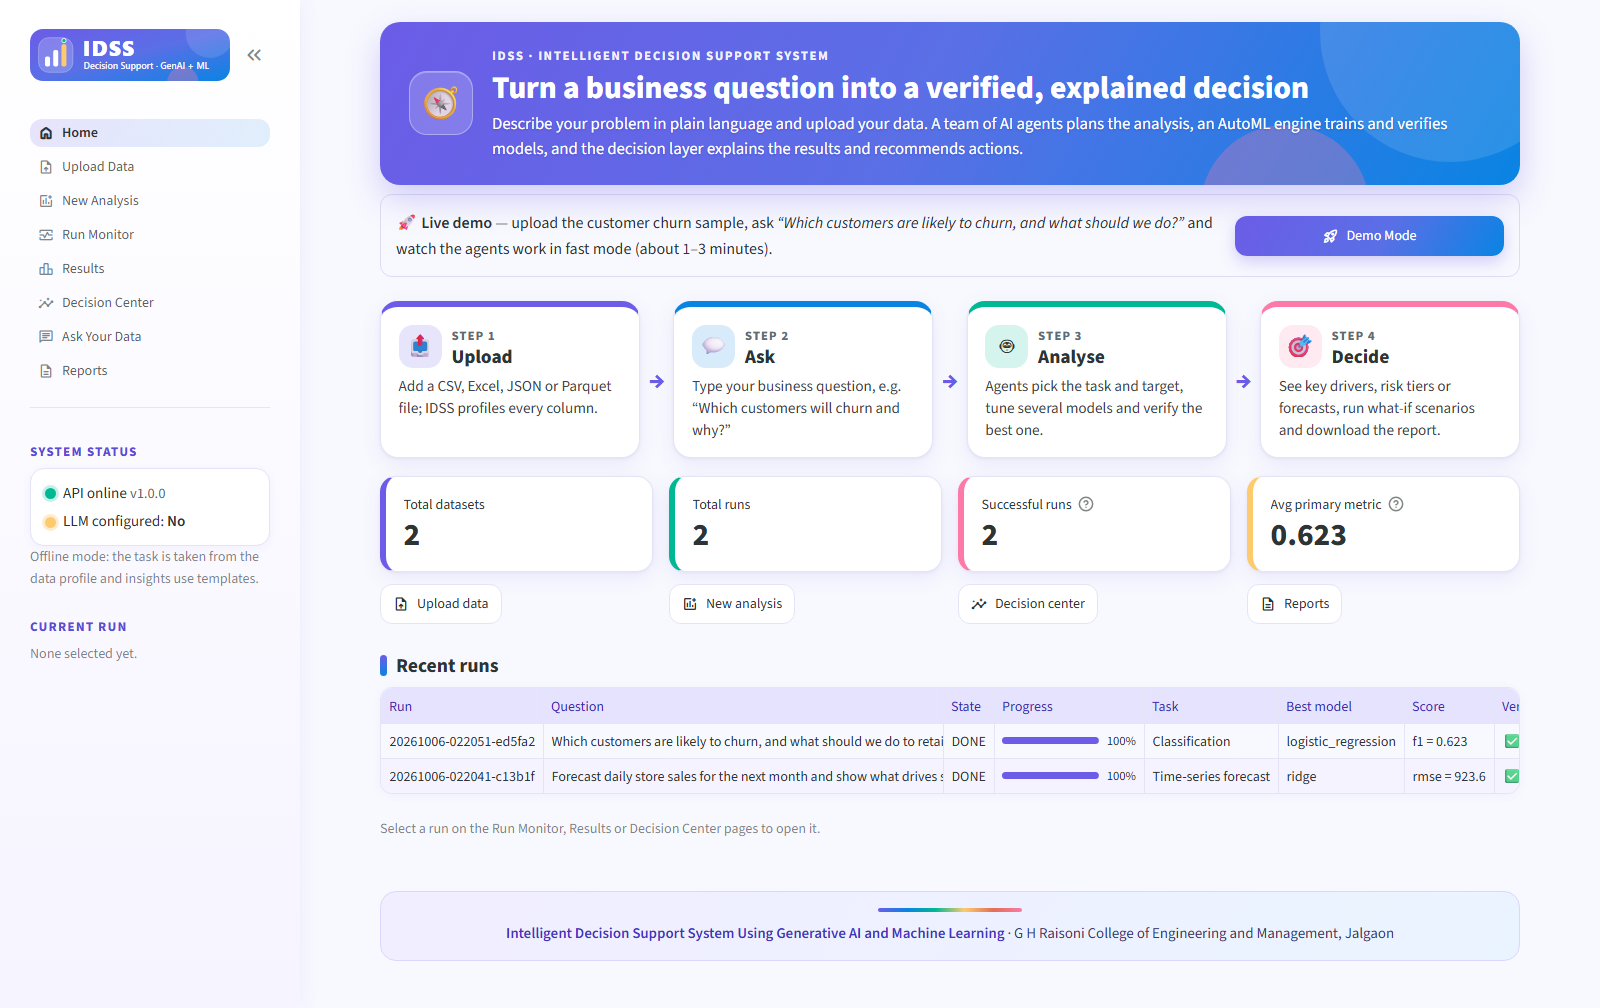
\includegraphics[width=\linewidth,height=7.3in,keepaspectratio]{figures/01_home.png}
  \caption{Home page: overview, Demo Mode, four-step flow, KPI strip and recent runs}\label{fig:5.1}
\end{figure}

\begin{figure}[htbp]
  \centering
  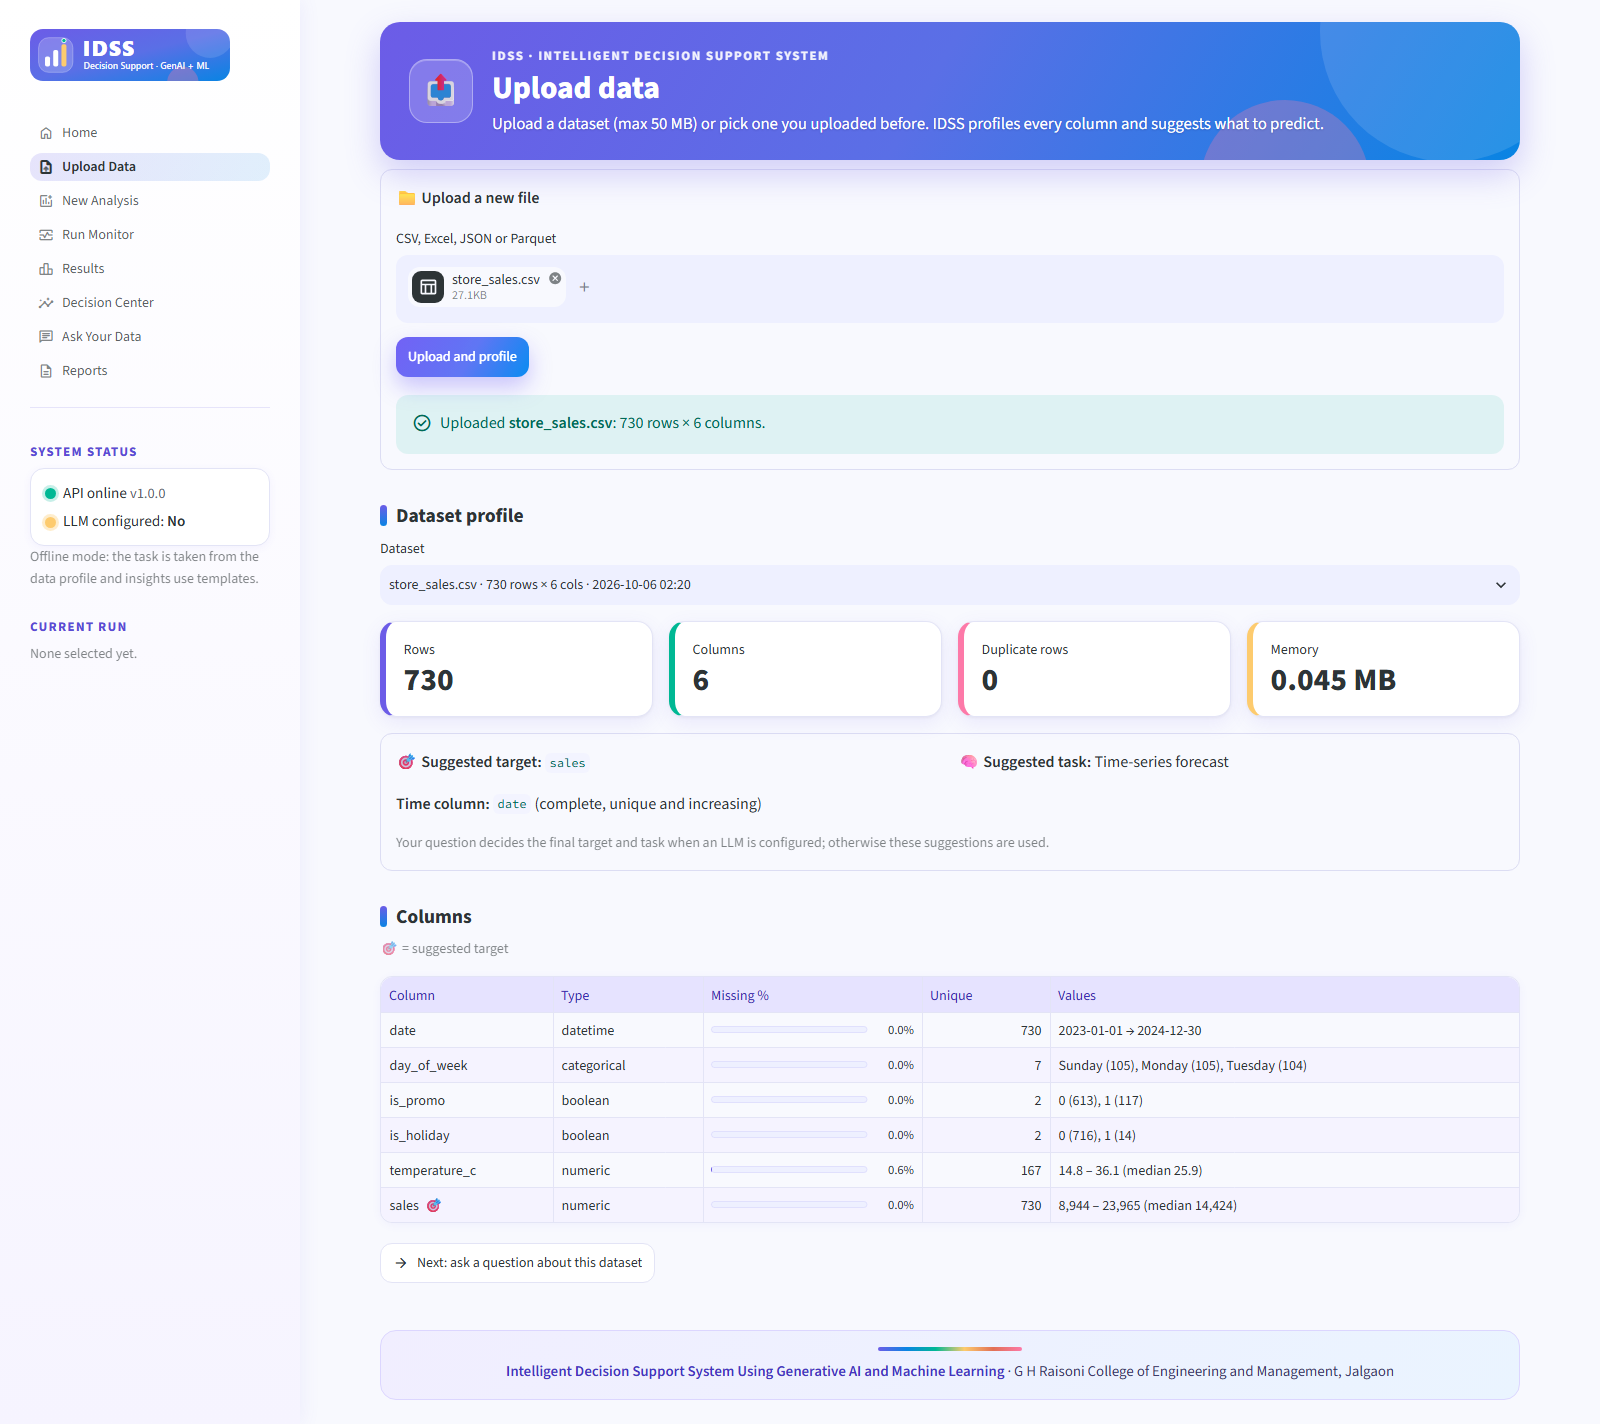
\includegraphics[width=\linewidth,height=7.3in,keepaspectratio]{figures/02_upload_profile.png}
  \caption{Upload Data page: profile of \code{store\_\allowbreak{}sales.csv} with types, missing values and suggested target and task}\label{fig:5.2}
\end{figure}

\begin{figure}[htbp]
  \centering
  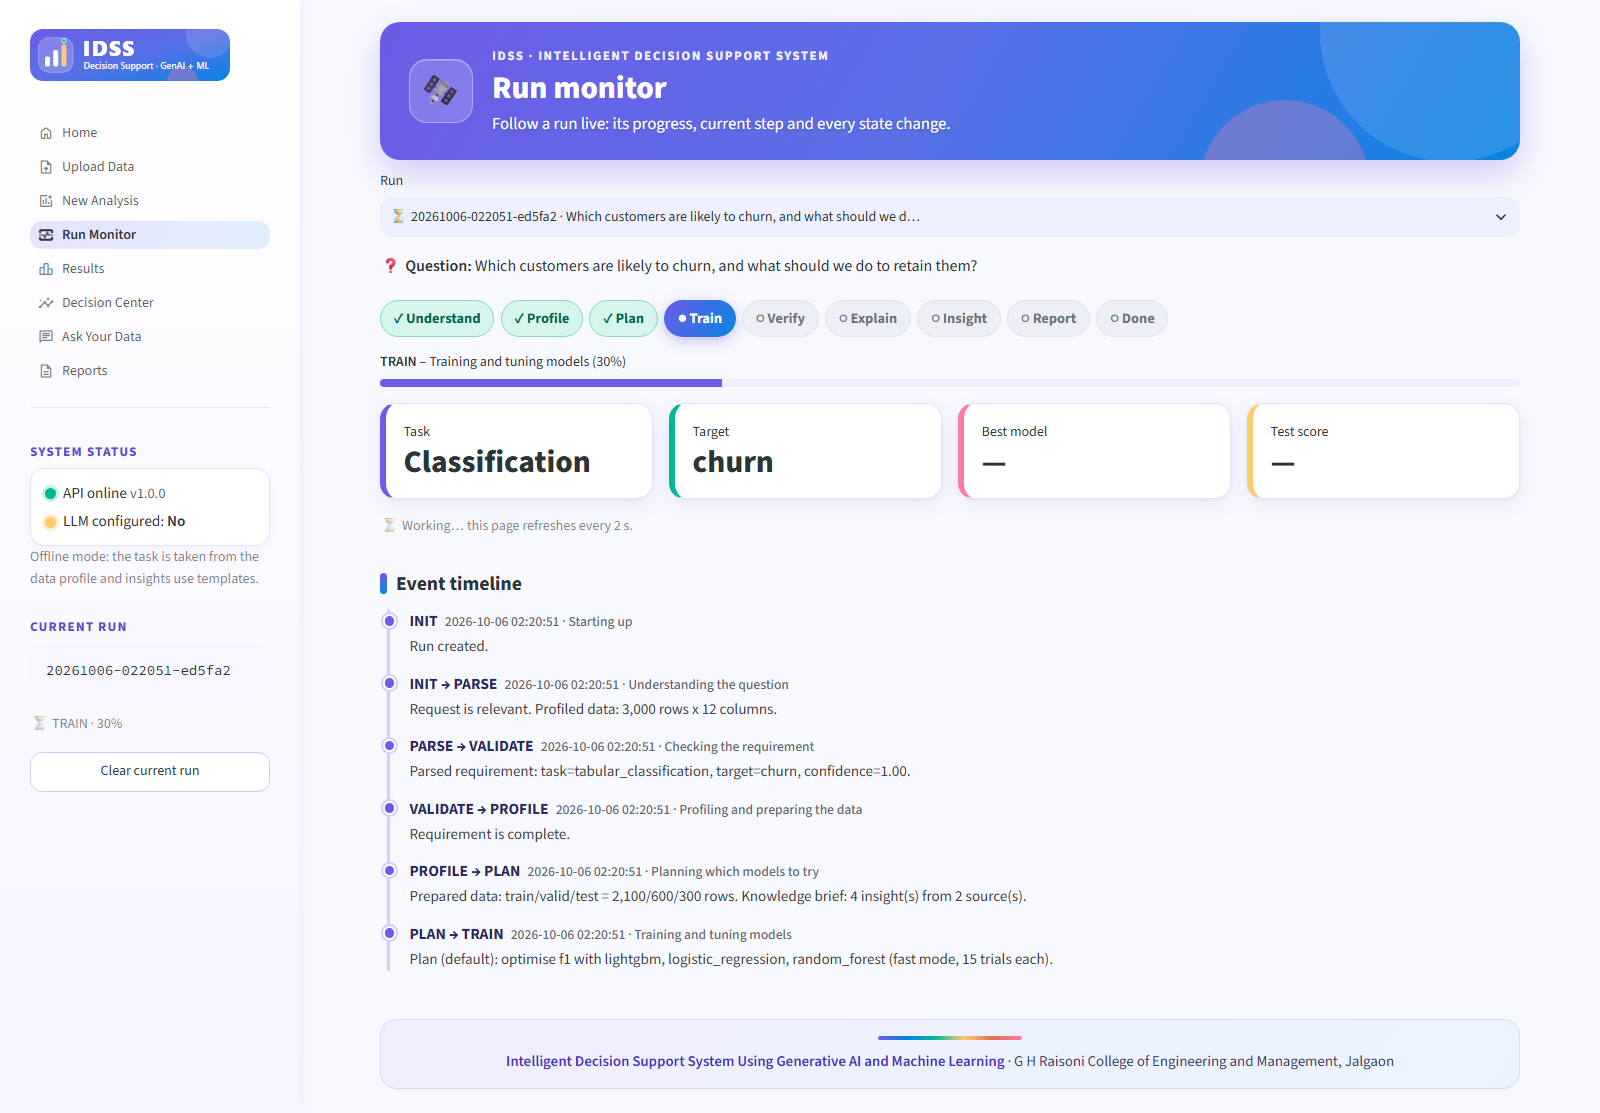
\includegraphics[width=\linewidth,height=7.3in,keepaspectratio]{figures/04_run_monitor.png}
  \caption{Run Monitor: pipeline stages, progress and event timeline of the churn run while it trains}\label{fig:5.3}
\end{figure}

\begin{figure}[htbp]
  \centering
  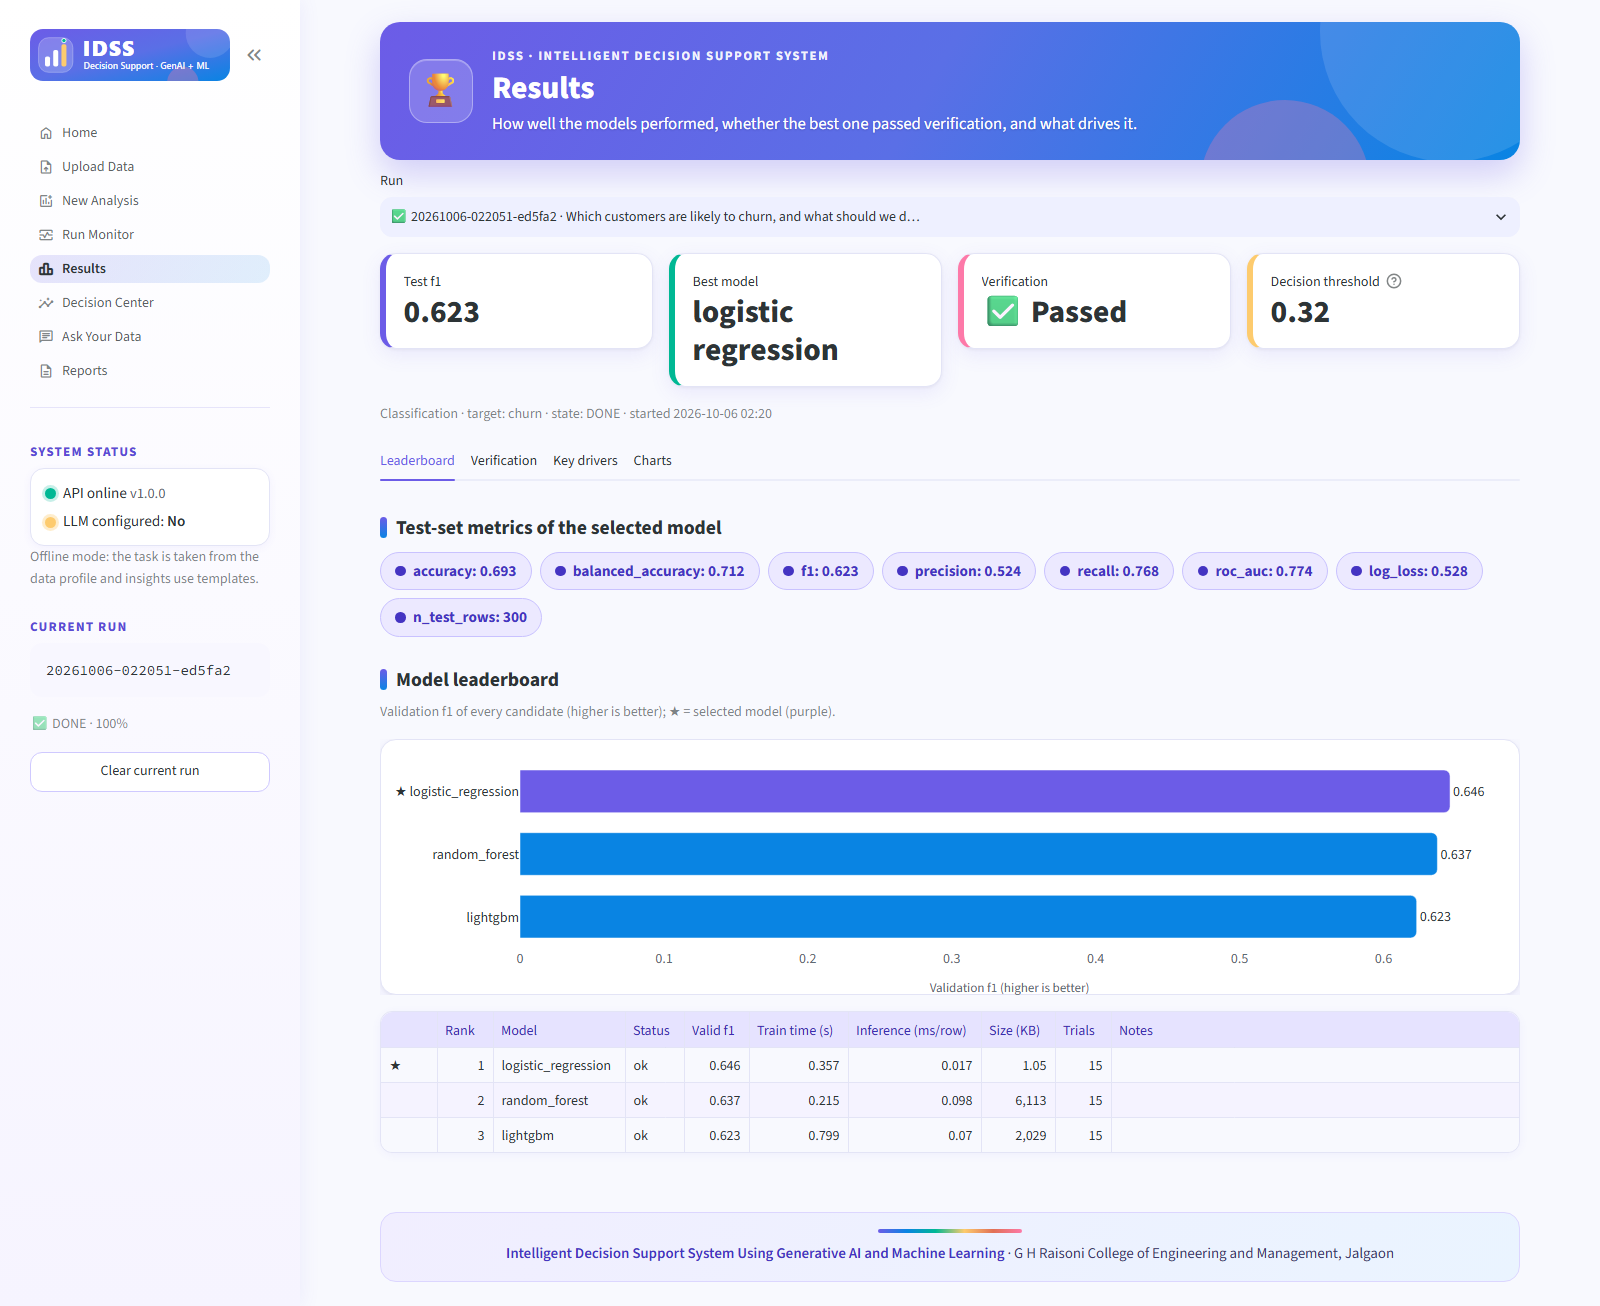
\includegraphics[width=\linewidth,height=7.3in,keepaspectratio]{figures/05_results.png}
  \caption{Results page: test metrics with leaderboard, verification, key-driver and chart tabs}\label{fig:5.4}
\end{figure}

\begin{figure}[htbp]
  \centering
  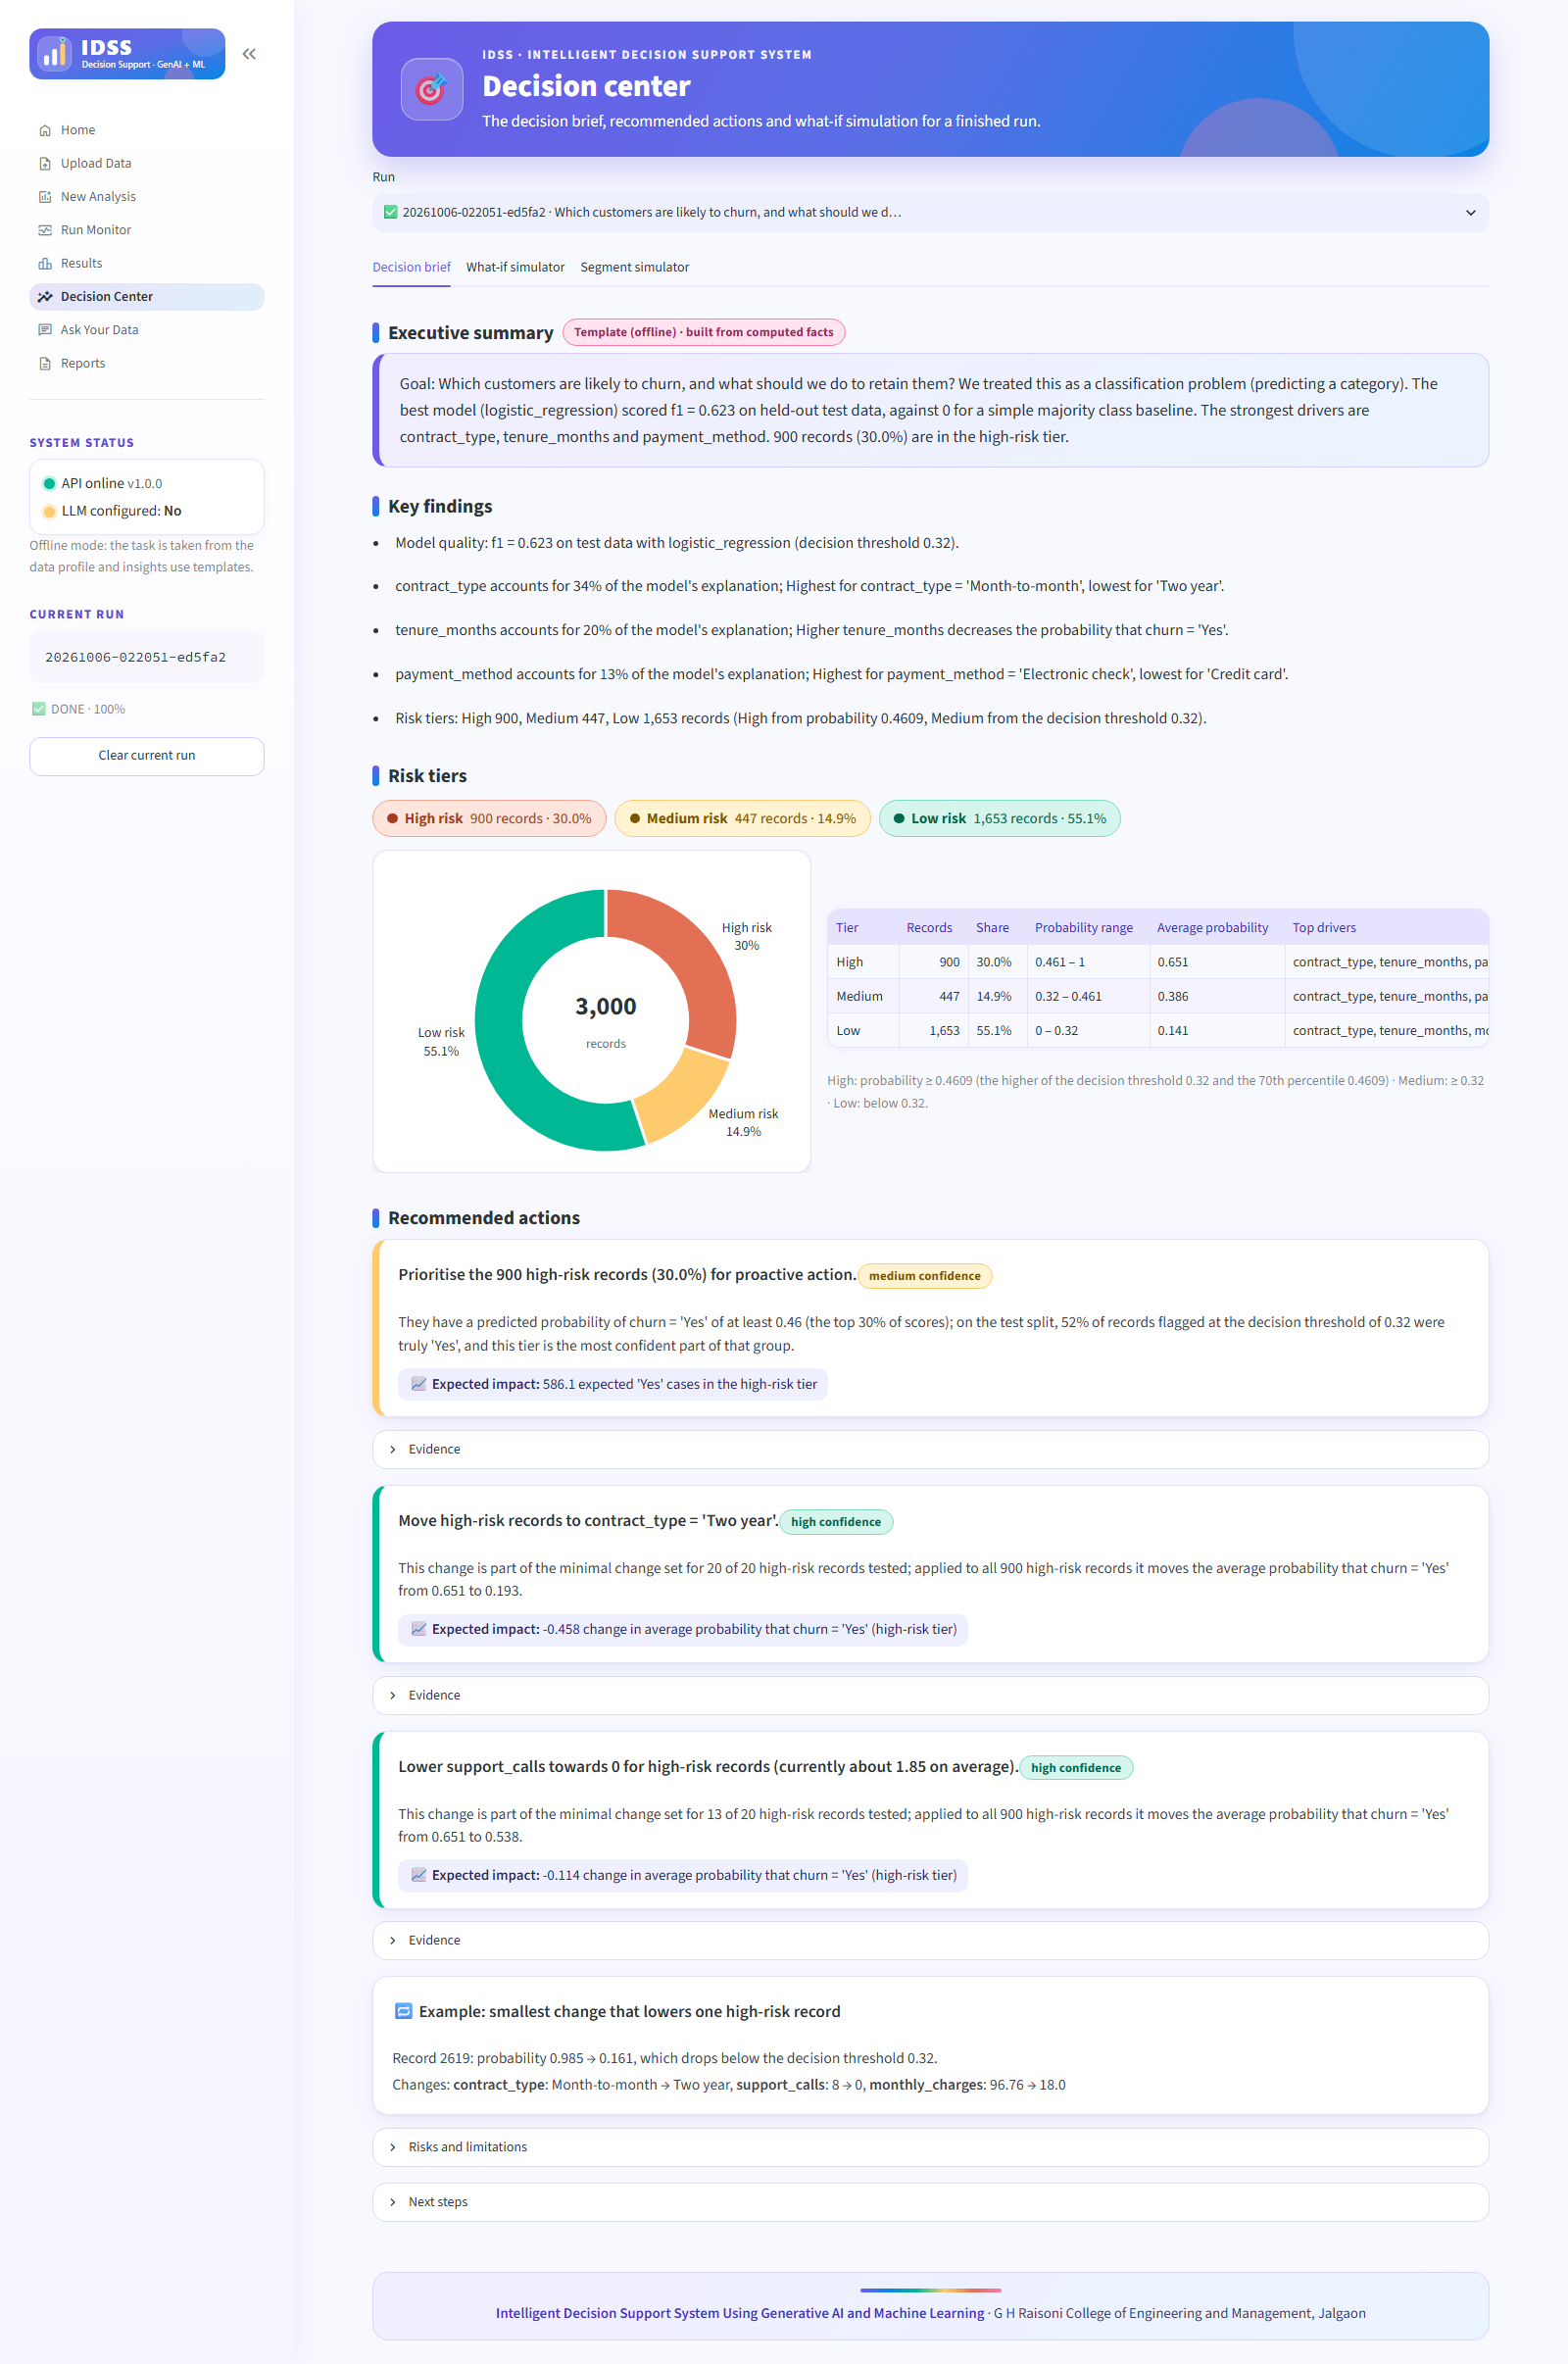
\includegraphics[width=\linewidth,height=7.3in,keepaspectratio]{figures/06_decision_center.png}
  \caption{Decision Center: executive summary, key findings, risk tiers and recommended actions for the churn run}\label{fig:5.5}
\end{figure}

\begin{figure}[htbp]
  \centering
  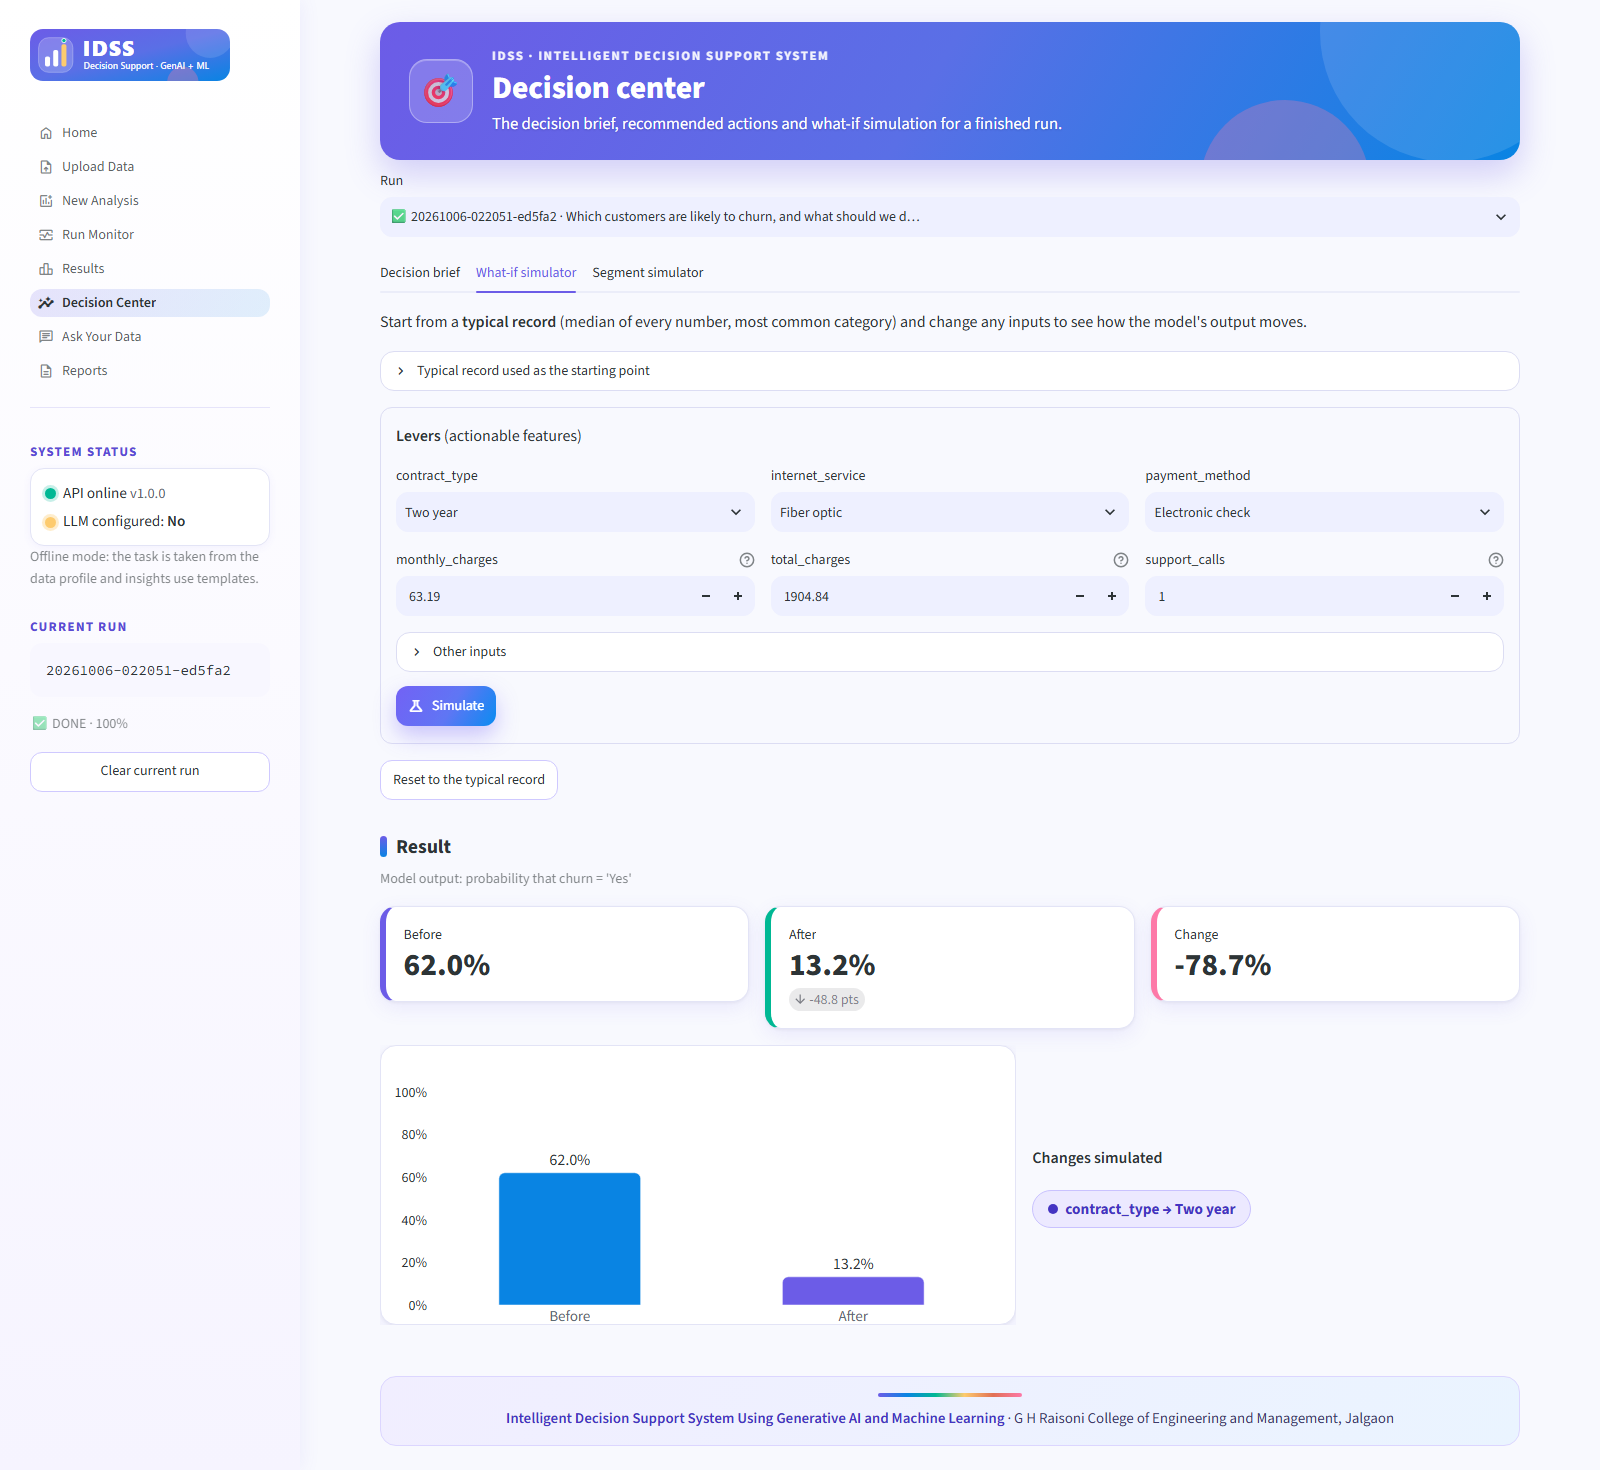
\includegraphics[width=\linewidth,height=7.3in,keepaspectratio]{figures/07_what_if.png}
  \caption{What-if simulator: a typical customer with \code{contract\_\allowbreak{}type} changed to ``Two year'', prediction before and after}\label{fig:5.6}
\end{figure}

\begin{figure}[htbp]
  \centering
  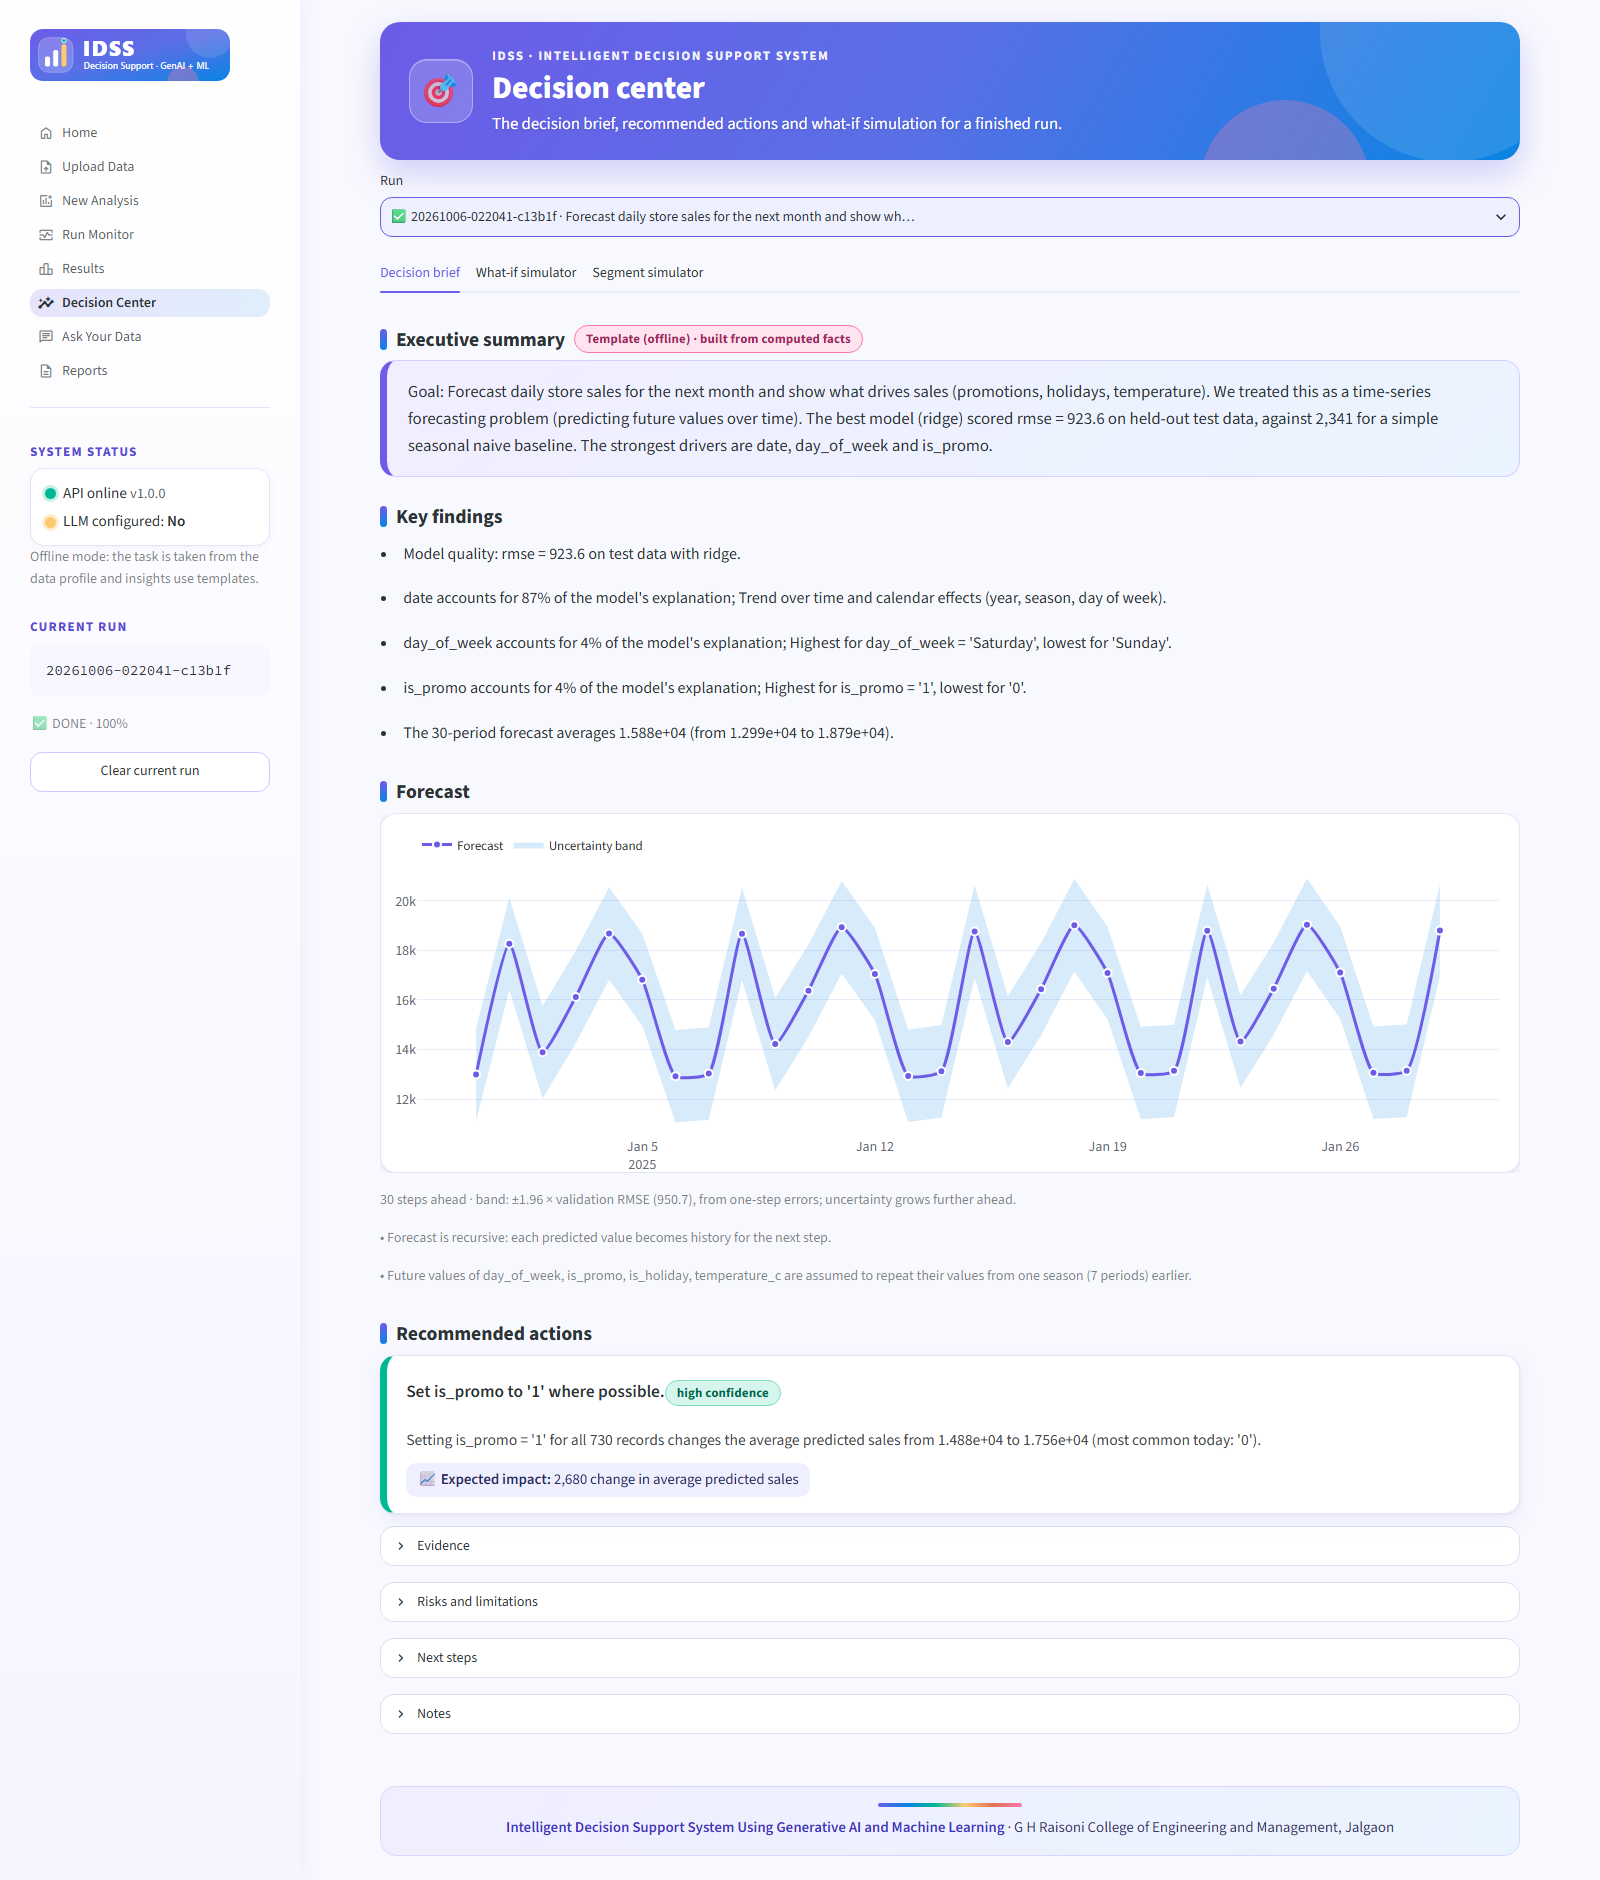
\includegraphics[width=\linewidth,height=7.3in,keepaspectratio]{figures/08_forecast.png}
  \caption{Decision Center for the store-sales run: forecast with its uncertainty band}\label{fig:5.7}
\end{figure}

\FloatBarrier
\section{Summary}\label{sec:5.6}

Eight algorithms capture the core logic: the state machine, requirement repair, the AutoML loop, threshold tuning, verification with re-planning, counterfactual search, the grounding check and the sandbox guard. Twelve modules implement them, each with a responsible member; short code extracts show how single use of the test split, contained failures, grounded numbers and sandboxed code are enforced; and the screenshots show the interface page by page.

% Generated by scripts/build_latex.py from docs/report/ch6_testing.md: edit the Markdown, not this file.
\chapter{Testing}\label{ch:6}

Testing was part of every weekly increment: no increment was closed until its own tests and the full existing suite passed. This chapter describes the black-box and white-box techniques, the automated and manual testing with their statistics and coverage, the identified test cases and the security tests.

\FloatBarrier
\section{Black Box, White Box Testing}\label{sec:6.1}

\textbf{Black-box tests} check what a component does through its public interface. The API is called with FastAPI's \code{TestClient} as the UI would call it, Streamlit pages are rendered with \code{AppTest} and inspected for what a user would see, and complete offline runs are checked for their final state and outputs. We used \textbf{equivalence partitioning} (supported and unsupported files; relevant and irrelevant questions), \textbf{boundary values} (an upload just over the limit; exactly two clarification rounds; fewer than 30 test rows) and \textbf{error guessing} (path-traversal strings, unknown ids, a stopped backend).

\textbf{White-box tests} use knowledge of the code to exercise paths and invariants: a spy confirms that the tuner only ever sees the training and validation splits, a handler that loops forever tests the step limit, each verification check is made to fail on its own, and one changed value in a time series proves that a lag feature never sees its own row. Coverage (Section~\ref{sec:6.2.3}) measures how much code the tests execute (Table~\ref{tab:6.1}).

\begin{table}[H]
\centering
\linespread{1}\small
\setlength{\tabcolsep}{4pt}
\caption{Black-box and white-box testing in IDSS}\label{tab:6.1}
\begin{tabular}{|>{\raggedright\arraybackslash\hspace{0pt}}p{\dimexpr 0.1687\linewidth-2\tabcolsep-2\arrayrulewidth\relax}|>{\raggedright\arraybackslash\hspace{0pt}}p{\dimexpr 0.4157\linewidth-2\tabcolsep-2\arrayrulewidth\relax}|>{\raggedright\arraybackslash\hspace{0pt}}p{\dimexpr 0.4157\linewidth-2\tabcolsep-2\arrayrulewidth\relax}|}
\hline
\rowcolor{tableheader}\textbf{Aspect} & \textbf{Black-box} & \textbf{White-box} \\
\hline
Basis & Requirements and public interfaces (API, UI, Orchestrator) & Branches, invariants and internal objects \\ \hline
Techniques & Equivalence partitioning, boundary values, error guessing, end-to-end scenarios & Spies and fakes, fault injection, invariant checks, coverage \\ \hline
Main files & \code{test\_\allowbreak{}api.py}, \code{test\_\allowbreak{}ui\_\allowbreak{}pages.py}, \code{test\_\allowbreak{}ui\_\allowbreak{}client.py} & \code{test\_\allowbreak{}automl.py}, \code{test\_\allowbreak{}step5.py}, \code{test\_\allowbreak{}requirement\_\allowbreak{}and\_\allowbreak{}manager.\allowbreak{}py}, \code{test\_\allowbreak{}data\_\allowbreak{}module.\allowbreak{}py} \\ \hline
\end{tabular}
\end{table}

\FloatBarrier
\section{Automated / Manual Testing}\label{sec:6.2}

\subsection{Automated Testing}\label{sec:6.2.1}

The pytest suite runs fully offline: every LLM call is replaced by a fake client (\code{tests/\allowbreak{}fakes.py}) that returns prepared structured outputs and records the prompts it received; web search is disabled and the workspace is redirected to a temporary folder (\code{tests/\allowbreak{}conftest.py}); training tests use tiny data and one or two Optuna trials. Tests that call a real LLM are marked \code{live} and deselected by default. \code{ruff} lints the whole code base. Two system-level runs complete the picture: \code{scripts/\allowbreak{}evaluate.\allowbreak{}py} runs the real Orchestrator end to end on five datasets with three seeds (Chapter~\ref{ch:7}), and \code{scripts/\allowbreak{}make\_\allowbreak{}screenshots.\allowbreak{}py} drives the running web interface in a real browser (Playwright) through an upload, two analyses, a what-if simulation and every page.

\subsection{Test Statistics}\label{sec:6.2.2}

The 228 test functions expand through parametrisation to \textbf{449 test cases}: \textbf{447 run offline} and 2 are live LLM tests. The final offline run gave \textbf{447 passed, 2 deselected, 0 failed} in 206.9 s (Table~\ref{tab:6.2}).

\begingroup
\linespread{1}\small
\setlength{\tabcolsep}{4pt}
\begin{longtable}{|>{\raggedright\arraybackslash\hspace{0pt}}p{\dimexpr 0.3286\linewidth-2\tabcolsep-2\arrayrulewidth\relax}|>{\raggedleft\arraybackslash\hspace{0pt}}p{\dimexpr 0.1005\linewidth-2\tabcolsep-2\arrayrulewidth\relax}|>{\raggedright\arraybackslash\hspace{0pt}}p{\dimexpr 0.5708\linewidth-2\tabcolsep-2\arrayrulewidth\relax}|}
\caption{Test inventory}\label{tab:6.2}\\
\hline
\rowcolor{tableheader}\textbf{Test file} & \textbf{Cases} & \textbf{Area} \\
\hline
\endfirsthead
\hline
\rowcolor{tableheader}\textbf{Test file} & \textbf{Cases} & \textbf{Area} \\
\endhead
\code{test\_\allowbreak{}foundation.py} & 36 & Settings, schemas, LLM client \\ \hline
\code{test\_\allowbreak{}data\_\allowbreak{}module.\allowbreak{}py} & 45 & Loader, profiler, preprocessing, splits, Data Agent \\ \hline
\code{test\_\allowbreak{}requirement\_\allowbreak{}and\_\allowbreak{}manager.\allowbreak{}py} & 36 & Prompts, Requirement Agent, state machine \\ \hline
\code{test\_\allowbreak{}automl.py} & 46 & Model zoo, tuner, trainer, Model Agent \\ \hline
\code{test\_\allowbreak{}step5.py} & 55 & Thresholds, retrieval, Verifier, sandbox, Analysis Agent, re-planning \\ \hline
\code{test\_\allowbreak{}step6.py} & 43 & Explanations, what-if, recommendations, insights, reports, offline runs \\ \hline
\code{test\_\allowbreak{}storage.py} & 6 & Repository and database mirroring \\ \hline
\code{test\_\allowbreak{}api.py} & 39 & Every endpoint and error case \\ \hline
\code{test\_\allowbreak{}ui\_\allowbreak{}client.py} & 18 & UI HTTP client \\ \hline
\code{test\_\allowbreak{}ui\_\allowbreak{}pages.py} & 106 & Every page, the theme and the chart builders \\ \hline
\code{test\_\allowbreak{}evaluation.py} & 17 & Ablation switches, baselines, SR / NPS / CS formulas, perturbations \\ \hline
\code{test\_\allowbreak{}live\_\allowbreak{}llm.py} & 2 & Real LLM smoke tests (only with \code{-m live}) \\ \hline
\textbf{Total} & \textbf{449} & \textbf{447 offline + 2 live} \\ \hline
\end{longtable}
\endgroup

\subsection{Code Coverage}\label{sec:6.2.3}

Coverage measured with pytest-cov over \code{idss}, \code{api}, \code{ui} and \code{configs} is \textbf{93\%} (6,494 statements, 468 not executed), as shown in Table~\ref{tab:6.3}.

\begin{table}[H]
\centering
\linespread{1}\small
\setlength{\tabcolsep}{4pt}
\caption{Code coverage per package}\label{tab:6.3}
\begin{tabular}{|>{\raggedright\arraybackslash\hspace{0pt}}p{\dimexpr 0.2231\linewidth-2\tabcolsep-2\arrayrulewidth\relax}|>{\raggedleft\arraybackslash\hspace{0pt}}p{\dimexpr 0.1687\linewidth-2\tabcolsep-2\arrayrulewidth\relax}|>{\raggedleft\arraybackslash\hspace{0pt}}p{\dimexpr 0.1142\linewidth-2\tabcolsep-2\arrayrulewidth\relax}|>{\raggedleft\arraybackslash\hspace{0pt}}p{\dimexpr 0.1414\linewidth-2\tabcolsep-2\arrayrulewidth\relax}|>{\raggedright\arraybackslash\hspace{0pt}}p{\dimexpr 0.3526\linewidth-2\tabcolsep-2\arrayrulewidth\relax}|}
\hline
\rowcolor{tableheader}\textbf{Package} & \textbf{Statements} & \textbf{Missed} & \textbf{Coverage} & \textbf{Note} \\
\hline
\code{idss/\allowbreak{}core} & 504 & 16 & 96.8\% &  \\ \hline
\code{idss/\allowbreak{}agents} & 1,185 & 53 & 95.5\% & Lowest: Analysis Agent (84\%) \\ \hline
\code{idss/\allowbreak{}ml} & 1,653 & 87 & 94.7\% &  \\ \hline
\code{idss/\allowbreak{}decision} & 668 & 36 & 94.6\% &  \\ \hline
\code{idss/\allowbreak{}knowledge} & 160 & 11 & 93.1\% & Web search providers 84\% (no network in tests) \\ \hline
\code{idss/\allowbreak{}storage} & 198 & 0 & 100\% &  \\ \hline
\code{idss/\allowbreak{}execution} & 168 & 86 & 48.8\% & \code{sandbox.py} 92\%; the runner (0\%) executes in a child process that coverage does not trace \\ \hline
\code{api} & 498 & 36 & 92.8\% & Lowest: background worker (80\%) \\ \hline
\code{ui} & 1,408 & 142 & 89.9\% & Lowest: Upload Data page (75\%) \\ \hline
\code{configs} & 51 & 1 & 98.0\% &  \\ \hline
\textbf{Total} & \textbf{6,494} & \textbf{468} & \textbf{93\%} &  \\ \hline
\end{tabular}
\end{table}

\subsection{Manual Testing}\label{sec:6.2.4}

Manual testing covered what needs human judgement --- whether texts are understandable, charts readable and the flow natural for a non-programmer. It was carried out during the Week 6--8 testing, as the decision layer, the API and the user interface became available, and followed the first-run scenario of Appendix~\ref{ch:A}: start the servers, run the churn example, follow the Run Monitor, read the results and verification, explore the Decision Center and a what-if change, and download the PDF. The command-line scripts of each increment (\code{demo\_\allowbreak{}step3.py}, \code{benchmark\_\allowbreak{}step4.py}, \code{demo\_\allowbreak{}step6.py}) served the same purpose for the engine; the saved Step 4 benchmark (\code{docs/\allowbreak{}results/\allowbreak{}step4\_\allowbreak{}benchmark.\allowbreak{}md}) is one recorded result.

\FloatBarrier
\section{Test Case Identification and Execution}\label{sec:6.3}

Table~\ref{tab:6.4} lists representative test cases derived from the requirements and risks; each is an automated test whose function is named in brackets. All passed in the final run.

\begingroup
\linespread{1}\small
\setlength{\tabcolsep}{4pt}
\begin{longtable}{|>{\raggedright\arraybackslash\hspace{0pt}}p{\dimexpr 0.0981\linewidth-2\tabcolsep-2\arrayrulewidth\relax}|>{\raggedright\arraybackslash\hspace{0pt}}p{\dimexpr 0.2176\linewidth-2\tabcolsep-2\arrayrulewidth\relax}|>{\raggedright\arraybackslash\hspace{0pt}}p{\dimexpr 0.2176\linewidth-2\tabcolsep-2\arrayrulewidth\relax}|>{\raggedright\arraybackslash\hspace{0pt}}p{\dimexpr 0.2176\linewidth-2\tabcolsep-2\arrayrulewidth\relax}|>{\raggedright\arraybackslash\hspace{0pt}}p{\dimexpr 0.1379\linewidth-2\tabcolsep-2\arrayrulewidth\relax}|>{\raggedright\arraybackslash\hspace{0pt}}p{\dimexpr 0.1111\linewidth-2\tabcolsep-2\arrayrulewidth\relax}|}
\caption{Test cases}\label{tab:6.4}\\
\hline
\rowcolor{tableheader}\textbf{ID} & \textbf{Module (test function)} & \textbf{Input} & \textbf{Expected output} & \textbf{Actual output} & \textbf{Result} \\
\hline
\endfirsthead
\hline
\rowcolor{tableheader}\textbf{ID} & \textbf{Module (test function)} & \textbf{Input} & \textbf{Expected output} & \textbf{Actual output} & \textbf{Result} \\
\endhead
TC-01 & LLM client (\code{test\_\allowbreak{}chat\_\allowbreak{}structured\_\allowbreak{}gives\_\allowbreak{}up\_\allowbreak{}after\_\allowbreak{}max\_\allowbreak{}retries}) & LLM always answers ``not json at all'' & 4 calls (1 + 3 retries), then a validation error with the raw output & As expected & Pass \\ \hline
TC-02 & Loader (\code{test\_\allowbreak{}load\_\allowbreak{}csv\_\allowbreak{}detects\_\allowbreak{}semicolon\_\allowbreak{}delimiter}) & CSV \code{a;b;c} with two rows & Columns a, b, c; shape (2, 3) & As expected & Pass \\ \hline
TC-03 & Split (\code{test\_\allowbreak{}split\_\allowbreak{}is\_\allowbreak{}stratified\_\allowbreak{}for\_\allowbreak{}classification}) & 1,000 rows, 20\% positives & 20\% \ensuremath{\pm}~1\% positives in every split & As expected & Pass \\ \hline
TC-04 & Split (\code{test\_\allowbreak{}split\_\allowbreak{}time\_\allowbreak{}series\_\allowbreak{}is\_\allowbreak{}chronological}) & 100 ordered rows & 70 / 20 / 10 rows; train before validation before test & As expected & Pass \\ \hline
TC-05 & Repair (\code{test\_\allowbreak{}repair\_\allowbreak{}replaces\_\allowbreak{}unusable\_\allowbreak{}target}, 2 cases) & Target \code{will\_\allowbreak{}leave} (absent) or \code{customer\_\allowbreak{}id} (an id) & Target becomes \code{churn} with an explanatory note & As expected & Pass \\ \hline
TC-06 & Orchestrator (\code{test\_\allowbreak{}irrelevant\_\allowbreak{}question\_\allowbreak{}ends\_\allowbreak{}politely\_\allowbreak{}without\_\allowbreak{}training}) & ``Hello! How is your day going?'' & INIT \ensuremath{\rightarrow} DONE, polite reply, no training & As expected & Pass \\ \hline
TC-07 & Orchestrator (\code{test\_\allowbreak{}revision\_\allowbreak{}limit\_\allowbreak{}fails\_\allowbreak{}the\_\allowbreak{}run}) & Vague question; two vague answers & NEEDS\_INPUT, then FAILED after 2 rounds; further answers rejected & As expected & Pass \\ \hline
TC-08 & Orchestrator (\code{test\_\allowbreak{}state\_\allowbreak{}is\_\allowbreak{}persisted\_\allowbreak{}and\_\allowbreak{}resumable}) & Run stopped at PROFILE, resumed by a new instance & \code{state.json} shows PROFILE; resumed run reaches DONE & As expected & Pass \\ \hline
TC-09 & Orchestrator (\code{test\_\allowbreak{}step\_\allowbreak{}limit\_\allowbreak{}stops\_\allowbreak{}a\_\allowbreak{}looping\_\allowbreak{}run}) & Handler that always returns TRAIN; limit 20 & FAILED with ``possible loop'' & As expected & Pass \\ \hline
TC-10 & Trainer (\code{test\_\allowbreak{}test\_\allowbreak{}split\_\allowbreak{}is\_\allowbreak{}untouched\_\allowbreak{}until\_\allowbreak{}final\_\allowbreak{}evaluation}) & 240 rows, 2 models & Tuning sees 168 / 48 rows only; test read once; 24 test rows & As expected & Pass \\ \hline
TC-11 & Time-series features (\code{test\_\allowbreak{}time\_\allowbreak{}series\_\allowbreak{}features\_\allowbreak{}use\_\allowbreak{}only\_\allowbreak{}past\_\allowbreak{}values}) & Day-30 sales raised by 1,000 & Features of days \ensuremath{\leq} 30 unchanged; day-31 lag-1 equals the new value & As expected & Pass \\ \hline
TC-12 & Selection (\code{test\_\allowbreak{}constraint\_\allowbreak{}violations\_\allowbreak{}are\_\allowbreak{}marked\_\allowbreak{}and\_\allowbreak{}avoided}) & Scores 0.90 at 8 ms/row and 0.80 at 0.5 ms/row; limit 5 ms & Faster model selected; violation recorded & As expected & Pass \\ \hline
TC-13 & Model Agent (\code{test\_\allowbreak{}model\_\allowbreak{}agent\_\allowbreak{}keeps\_\allowbreak{}only\_\allowbreak{}zoo\_\allowbreak{}names}) & LLM ranks ``XGBoost'', ``svm'', ``Random Forest'' & Unknown ``svm'' dropped with a note; zoo models completed & As expected & Pass \\ \hline
TC-14 & Threshold (\code{test\_\allowbreak{}tune\_\allowbreak{}threshold\_\allowbreak{}finds\_\allowbreak{}a\_\allowbreak{}better\_\allowbreak{}cutoff}) & 15\% positives with probabilities mostly below 0.5 & Threshold \textless{} 0.5 and higher F1 than at 0.5 & As expected & Pass \\ \hline
TC-15 & Verifier (\code{test\_\allowbreak{}verifier\_\allowbreak{}detects\_\allowbreak{}each\_\allowbreak{}problem}, 8 cases) & One defect at a time (target missed, baseline not beaten, constraint, 20 test rows, test read twice, leakage, over-fitting, \ldots{}) & Fails with exactly that check and its recommendation & As expected & Pass \\ \hline
TC-16 & Re-planning (\code{test\_\allowbreak{}failed\_\allowbreak{}verification\_\allowbreak{}replans\_\allowbreak{}at\_\allowbreak{}most\_\allowbreak{}once}) & Verifier that always fails & Two PLAN / TRAIN / VERIFY rounds, then DONE flagged not verified; full budget on re-plan & As expected & Pass \\ \hline
TC-17 & Explanations (\code{test\_\allowbreak{}derived\_\allowbreak{}columns\_\allowbreak{}fold\_\allowbreak{}back\_\allowbreak{}to\_\allowbreak{}original\_\allowbreak{}names}) & One-hot and lag / calendar features & Drivers named \code{region}, \code{sales (history)}, \code{date}, \code{promo} & As expected & Pass \\ \hline
TC-18 & What-if (\code{test\_\allowbreak{}what\_\allowbreak{}if\_\allowbreak{}rejects\_\allowbreak{}invalid\_\allowbreak{}changes}, 6 cases) & Text for a number, \% on a category, unknown column, target, empty, bad kind & \code{WhatIfError} for each & As expected & Pass \\ \hline
TC-19 & Counterfactual (\code{test\_\allowbreak{}counterfactual\_\allowbreak{}lowers\_\allowbreak{}risk\_\allowbreak{}using\_\allowbreak{}actionable\_\allowbreak{}features\_\allowbreak{}only}) & Riskiest record & Below threshold with 1--3 changes to observed values & As expected & Pass \\ \hline
TC-20 & Risk tiers (\code{test\_\allowbreak{}tier\_\allowbreak{}cutoffs\_\allowbreak{}use\_\allowbreak{}threshold\_\allowbreak{}and\_\allowbreak{}percentile}, 2 cases) & 1,000 probabilities; threshold 0.2 or 0.85 & High cut-off 0.6993 or 0.85; counts (300, 500, 200) or (150, 0, 850) & As expected & Pass \\ \hline
TC-21 & Grounding (\code{test\_\allowbreak{}invented\_\allowbreak{}number\_\allowbreak{}triggers\_\allowbreak{}one\_\allowbreak{}regeneration\_\allowbreak{}then\_\allowbreak{}template}) & LLM twice writes ``Churn will fall by 37.5\% next quarter.'' & One regeneration naming 37.5\%, then the template brief & As expected & Pass \\ \hline
TC-22 & Storage (\code{test\_\allowbreak{}database\_\allowbreak{}failure\_\allowbreak{}never\_\allowbreak{}stops\_\allowbreak{}a\_\allowbreak{}run}) & Repository failing on every call & Run still reaches DONE & As expected & Pass \\ \hline
TC-23 & API (\code{test\_\allowbreak{}second\_\allowbreak{}run\_\allowbreak{}while\_\allowbreak{}busy\_\allowbreak{}returns\_\allowbreak{}409}) & Second run and a what-if during a run & \code{409 busy}, \code{409 run\_\allowbreak{}in\_\allowbreak{}progress}; \code{/health} still answers & As expected & Pass \\ \hline
TC-24 & UI (\code{test\_\allowbreak{}every\_\allowbreak{}page\_\allowbreak{}handles\_\allowbreak{}backend\_\allowbreak{}down}, 8 pages) & Backend stopped & Every page shows ``API offline'' and the start hint & As expected & Pass \\ \hline
\end{longtable}
\endgroup

\FloatBarrier
\section{Security Testing}\label{sec:6.4}

\begingroup
\linespread{1}\small
\setlength{\tabcolsep}{4pt}
\begin{longtable}{|>{\raggedright\arraybackslash\hspace{0pt}}p{\dimexpr 0.1005\linewidth-2\tabcolsep-2\arrayrulewidth\relax}|>{\raggedright\arraybackslash\hspace{0pt}}p{\dimexpr 0.1863\linewidth-2\tabcolsep-2\arrayrulewidth\relax}|>{\raggedright\arraybackslash\hspace{0pt}}p{\dimexpr 0.2383\linewidth-2\tabcolsep-2\arrayrulewidth\relax}|>{\raggedright\arraybackslash\hspace{0pt}}p{\dimexpr 0.2383\linewidth-2\tabcolsep-2\arrayrulewidth\relax}|>{\raggedright\arraybackslash\hspace{0pt}}p{\dimexpr 0.2364\linewidth-2\tabcolsep-2\arrayrulewidth\relax}|}
\caption{Security tests (all passed)}\label{tab:6.5}\\
\hline
\rowcolor{tableheader}\textbf{ID} & \textbf{Threat} & \textbf{Test function} & \textbf{Input} & \textbf{Expected and actual result} \\
\hline
\endfirsthead
\hline
\rowcolor{tableheader}\textbf{ID} & \textbf{Threat} & \textbf{Test function} & \textbf{Input} & \textbf{Expected and actual result} \\
\endhead
ST-01 & Unsafe LLM-written code & \code{test\_\allowbreak{}sandbox\_\allowbreak{}blocks\_\allowbreak{}unsafe\_\allowbreak{}code\_\allowbreak{}before\_\allowbreak{}running} (15 cases) & \code{import os}, \code{import subprocess}, \code{open(...)}, \code{eval(...)}, \code{\_\_import\_\allowbreak{}\_\allowbreak{}('os')}, \code{().\_\allowbreak{}\_\allowbreak{}class\_\_}, \code{pd.read\_\allowbreak{}csv(...)}, \code{df.to\_\allowbreak{}csv(...)}, \code{np.load(...)}, \ldots{} & Blocked by the static guard in under 1 s, nothing executed \\ \hline
ST-02 & Endless loop & \code{test\_\allowbreak{}sandbox\_\allowbreak{}kills\_\allowbreak{}infinite\_\allowbreak{}loops} & \code{while True: pass}, 3 s timeout & Process stopped; ``Timed out after 3s'' \\ \hline
ST-03 & Output flooding & \code{test\_\allowbreak{}sandbox\_\allowbreak{}truncates\_\allowbreak{}huge\_\allowbreak{}output} & \code{print('x' }\code{*}\code{ 100\_\allowbreak{}000)} & Output cut to 20 KB; result still returned \\ \hline
ST-04 & Key leakage to the sandbox & \code{test\_\allowbreak{}sandbox\_\allowbreak{}child\_\allowbreak{}gets\_\allowbreak{}no\_\allowbreak{}secrets} & \code{LLM\_\allowbreak{}API\_\allowbreak{}KEY}, \code{TAVILY\_\allowbreak{}API\_\allowbreak{}KEY} set & Neither present in the child environment \\ \hline
ST-05 & Path traversal (charts) & \code{test\_\allowbreak{}chart\_\allowbreak{}path\_\allowbreak{}traversal\_\allowbreak{}is\_\allowbreak{}blocked} (6 cases) & \code{charts/\allowbreak{}.\allowbreak{}.\allowbreak{}\%5C.\allowbreak{}.\allowbreak{}\%5Cstate.\allowbreak{}json}, \code{charts/\allowbreak{}\%2E\%2E/\allowbreak{}\%2E\%2E/\allowbreak{}state.\allowbreak{}json}, \ldots{} & \code{400} / \code{404}; \code{state.json} never returned \\ \hline
ST-06 & Path tricks in run ids & \code{test\_\allowbreak{}run\_\allowbreak{}id\_\allowbreak{}path\_\allowbreak{}tricks\_\allowbreak{}are\_\allowbreak{}rejected} & \code{..\%5C.\allowbreak{}.\allowbreak{}\%5Cworkspace}, \code{..} & \code{404} \\ \hline
ST-07 & Malicious file names & \code{test\_\allowbreak{}sanitize\_\allowbreak{}filename} (6 cases) & \code{../\allowbreak{}.\allowbreak{}.\allowbreak{}/\allowbreak{}etc/\allowbreak{}passwd.\allowbreak{}csv}, a 300-character name, \ldots{} & \code{passwd.csv}; names shortened to 80 characters \\ \hline
ST-08 & Bad or oversized uploads & \code{test\_\allowbreak{}upload\_\allowbreak{}rejects\_\allowbreak{}unsupported\_\allowbreak{}extensions}, \code{test\_\allowbreak{}upload\_\allowbreak{}rejects\_\allowbreak{}files\_\allowbreak{}over\_\allowbreak{}the\_\allowbreak{}limit} & \code{data.csv.exe}; files above the limit & \code{415}; \code{413} checked before and while reading, partial file deleted \\ \hline
ST-09 & Key exposure by the API & \code{test\_\allowbreak{}health\_\allowbreak{}reports\_\allowbreak{}llm\_\allowbreak{}flag\_\allowbreak{}but\_\allowbreak{}never\_\allowbreak{}the\_\allowbreak{}key} & Secret key configured & \code{/health} shows only \code{llm\_\allowbreak{}configured: true} \\ \hline
ST-10 & Raw data sent to the LLM & \code{test\_\allowbreak{}prompts\_\allowbreak{}include\_\allowbreak{}profile\_\allowbreak{}summary\_\allowbreak{}but\_\allowbreak{}never\_\allowbreak{}raw\_\allowbreak{}values} & Churn profile in the parsing prompt & Column summary present; raw values such as \code{CUST-00001} absent \\ \hline
\end{longtable}
\endgroup

\FloatBarrier
\section{Summary}\label{sec:6.5}

IDSS was tested with black-box techniques through the API and the UI and with white-box techniques inside the engine. The automated suite has 449 test cases, of which all 447 offline cases passed, covering 93\% of 6,494 statements. Twenty-four representative test cases and ten security tests --- sandbox, path traversal, uploads and key leakage --- were documented with their inputs and results, and system-level runs and manual walk-throughs completed the testing.

% Generated by scripts/build_latex.py from docs/report/ch7_results.md: edit the Markdown, not this file.
\chapter{Results and Discussion}\label{ch:7}

All numbers in this chapter come from the offline evaluation script \code{scripts/\allowbreak{}evaluate.\allowbreak{}py} (full output in \code{docs/\allowbreak{}results/\allowbreak{}evaluation.\allowbreak{}md} and \code{evaluation.json}) and from the Step 4 / Step 5 benchmark (\code{docs/\allowbreak{}results/\allowbreak{}step4\_\allowbreak{}benchmark.\allowbreak{}md}).

\FloatBarrier
\section{Experimental Setup}\label{sec:7.1}

\textbf{Datasets.} We generated five datasets ourselves with \code{scripts/\allowbreak{}make\_\allowbreak{}samples.\allowbreak{}py} from fixed random seeds (Table~\ref{tab:7.1}). \textbf{All five are synthetic}: they describe no real people or companies and their generating processes are known. They were designed to be realistic in shape --- missing values, categorical columns, class imbalance, seasonality, overlapping clusters --- and to cover the four task families.

\begin{table}[H]
\centering
\linespread{1}\footnotesize
\setlength{\tabcolsep}{4pt}
\caption{Evaluation datasets (synthetic, seeded)}\label{tab:7.1}
\begin{tabular}{|>{\raggedright\arraybackslash\hspace{0pt}}p{\dimexpr 0.1216\linewidth-2\tabcolsep-2\arrayrulewidth\relax}|>{\raggedright\arraybackslash\hspace{0pt}}p{\dimexpr 0.1903\linewidth-2\tabcolsep-2\arrayrulewidth\relax}|>{\raggedleft\arraybackslash\hspace{0pt}}p{\dimexpr 0.0873\linewidth-2\tabcolsep-2\arrayrulewidth\relax}|>{\raggedleft\arraybackslash\hspace{0pt}}p{\dimexpr 0.1101\linewidth-2\tabcolsep-2\arrayrulewidth\relax}|>{\raggedright\arraybackslash\hspace{0pt}}p{\dimexpr 0.1903\linewidth-2\tabcolsep-2\arrayrulewidth\relax}|>{\raggedright\arraybackslash\hspace{0pt}}p{\dimexpr 0.1903\linewidth-2\tabcolsep-2\arrayrulewidth\relax}|>{\raggedright\arraybackslash\hspace{0pt}}p{\dimexpr 0.1102\linewidth-2\tabcolsep-2\arrayrulewidth\relax}|}
\hline
\rowcolor{tableheader}\textbf{Dataset} & \textbf{File} & \textbf{Rows} & \textbf{Columns} & \textbf{Task} & \textbf{Target} & \textbf{Notes} \\
\hline
Churn & \code{customer\_\allowbreak{}churn.csv} & 3,000 & 12 & Binary classification & \code{churn} & 985 ``Yes'' (32.8\%) \\ \hline
Crop price & \code{crop\_\allowbreak{}price.csv} & 2,000 & 11 & Regression & \code{price} & 106 missing cells \\ \hline
Store sales & \code{store\_\allowbreak{}sales.csv} & 730 & 6 & Forecasting & \code{sales} & Daily, two years \\ \hline
Delivery & \code{delivery\_\allowbreak{}status.\allowbreak{}csv} & 2,500 & 12 & 3-class classification & \code{delivery\_\allowbreak{}status} & 1,375 / 750 / 375 \\ \hline
Segments & \code{customer\_\allowbreak{}segments.\allowbreak{}csv} & 1,600 & 8 & Clustering & \code{segment} (scoring only) & Four groups \\ \hline
\end{tabular}
\end{table}

\textbf{Protocol.} Three seeds (42, 43, 44); every number is the mean \ensuremath{\pm}~sample standard deviation. The seed controls the split (chronological for time series), Optuna's sampler, the models and the perturbations. The \textbf{fast} budget was used (3 models \ensuremath{\times} 15 trials, 60 s per model, 180 s total; one re-plan with the full budget after a failed verification). The real Orchestrator ran in \textbf{offline mode}: requirements came from the data profile, and Segments was given an explicit clustering requirement whose \code{segment} column is used only for scoring. Models were selected on the validation split and the test split (10\%) was read once. \textbf{Environment:} Python 3.12.0, Windows 11, 16 logical CPUs, scikit-learn 1.9.1, XGBoost 3.4.1, LightGBM 4.7.0, Optuna 5.0.0, SHAP 0.52.0. The evaluation took 1,081.5 s, plus two short Segments re-runs (Section~\ref{sec:7.7}).

\textbf{Metrics.} F1 for classification (binary F1 of the positive class; weighted F1 for Delivery), RMSE for regression and forecasting, and the adjusted Rand index (ARI) for clustering. Each model is compared with a trivial baseline on the same test split: the majority class, the mean, the seasonal naive forecast or a random cluster assignment.

\FloatBarrier
\section{Main Benchmark}\label{sec:7.2}

\begin{table}[H]
\centering
\linespread{1}\fontsize{9}{11}\selectfont
\setlength{\tabcolsep}{3pt}
\caption{Main benchmark (full system, clean data, mean \ensuremath{\pm}~std over 3 seeds)}\label{tab:7.2}
\begin{tabular}{|>{\raggedright\arraybackslash\hspace{0pt}}p{\dimexpr 0.1134\linewidth-2\tabcolsep-2\arrayrulewidth\relax}|>{\raggedright\arraybackslash\hspace{0pt}}p{\dimexpr 0.1342\linewidth-2\tabcolsep-2\arrayrulewidth\relax}|>{\raggedright\arraybackslash\hspace{0pt}}p{\dimexpr 0.0927\linewidth-2\tabcolsep-2\arrayrulewidth\relax}|>{\raggedleft\arraybackslash\hspace{0pt}}p{\dimexpr 0.0822\linewidth-2\tabcolsep-2\arrayrulewidth\relax}|>{\raggedleft\arraybackslash\hspace{0pt}}p{\dimexpr 0.1134\linewidth-2\tabcolsep-2\arrayrulewidth\relax}|>{\raggedleft\arraybackslash\hspace{0pt}}p{\dimexpr 0.1446\linewidth-2\tabcolsep-2\arrayrulewidth\relax}|>{\raggedleft\arraybackslash\hspace{0pt}}p{\dimexpr 0.0822\linewidth-2\tabcolsep-2\arrayrulewidth\relax}|>{\raggedleft\arraybackslash\hspace{0pt}}p{\dimexpr 0.1238\linewidth-2\tabcolsep-2\arrayrulewidth\relax}|>{\raggedleft\arraybackslash\hspace{0pt}}p{\dimexpr 0.1136\linewidth-2\tabcolsep-2\arrayrulewidth\relax}|}
\hline
\rowcolor{tableheader}\textbf{Dataset} & \textbf{Best model (seeds)} & \textbf{Metric} & \textbf{Test score} & \textbf{Baseline} & \textbf{Improvement} & \textbf{Train time (s)} & \textbf{Inference (ms/row)} & \textbf{Verified} \\
\hline
Churn & logistic regression (3/3) & F1 \ensuremath{\uparrow} & 0.649 \ensuremath{\pm}~0.028 & 0.000 & n/a\textsuperscript{1} & 19.8 \ensuremath{\pm}~2.5 & 0.0286 \ensuremath{\pm}~0.0045 & 3/3 \\ \hline
Crop price & LightGBM (3/3) & RMSE \ensuremath{\downarrow} & 356.9 \ensuremath{\pm}~26.81 & 2,392.8 \ensuremath{\pm}~45.77 & +85.1\% \ensuremath{\pm}~0.8 & 7.0 \ensuremath{\pm}~0.5 & 0.0610 \ensuremath{\pm}~0.0073 & 3/3 \\ \hline
Store sales & ridge (3/3) & RMSE \ensuremath{\downarrow} & 923.6 \ensuremath{\pm}~0.000 & 2,340.7 \ensuremath{\pm}~0.000 & +60.5\% \ensuremath{\pm}~0.0 & 4.3 \ensuremath{\pm}~1.1 & 0.2011 \ensuremath{\pm}~0.0148 & 3/3 \\ \hline
Delivery & logistic regression (2/3) & F1 \ensuremath{\uparrow} & 0.656 \ensuremath{\pm}~0.024 & 0.393 \ensuremath{\pm}~0.000 & +67.0\% \ensuremath{\pm}~6.1 & 72.2 \ensuremath{\pm}~74.2 & 0.0440 \ensuremath{\pm}~0.0226 & 2/3 \\ \hline
Segments & Gaussian mixture (3/3) & ARI \ensuremath{\uparrow} & 0.816 \ensuremath{\pm}~0.045 & 0.004 \ensuremath{\pm}~0.007 & n/a\textsuperscript{1} & 2.7 \ensuremath{\pm}~0.4 & 0.0159 \ensuremath{\pm}~0.0036 & 3/3 \\ \hline
\end{tabular}
\end{table}

\ensuremath{\uparrow} higher is better, \ensuremath{\downarrow} lower is better. \textit{Train time} covers the whole search plus the final refit; \textit{inference} is the median time of the fitted pipeline on up to 500 test rows. \textsuperscript{1} The baseline is at chance level (below 0.05), so a relative improvement is undefined: the majority class never predicts churn (F1 = 0) and random clusters have an ARI of about 0.

The full system \textbf{beat the baseline on all five datasets}, reducing RMSE by 85.1\% on crop price and 60.5\% on store sales. Simple models were often selected --- logistic regression on churn and delivery, ridge on store sales --- which suggests that these synthetic datasets are close to linear (Figure~\ref{fig:7.1}).

\begin{figure}[htbp]
  \centering
  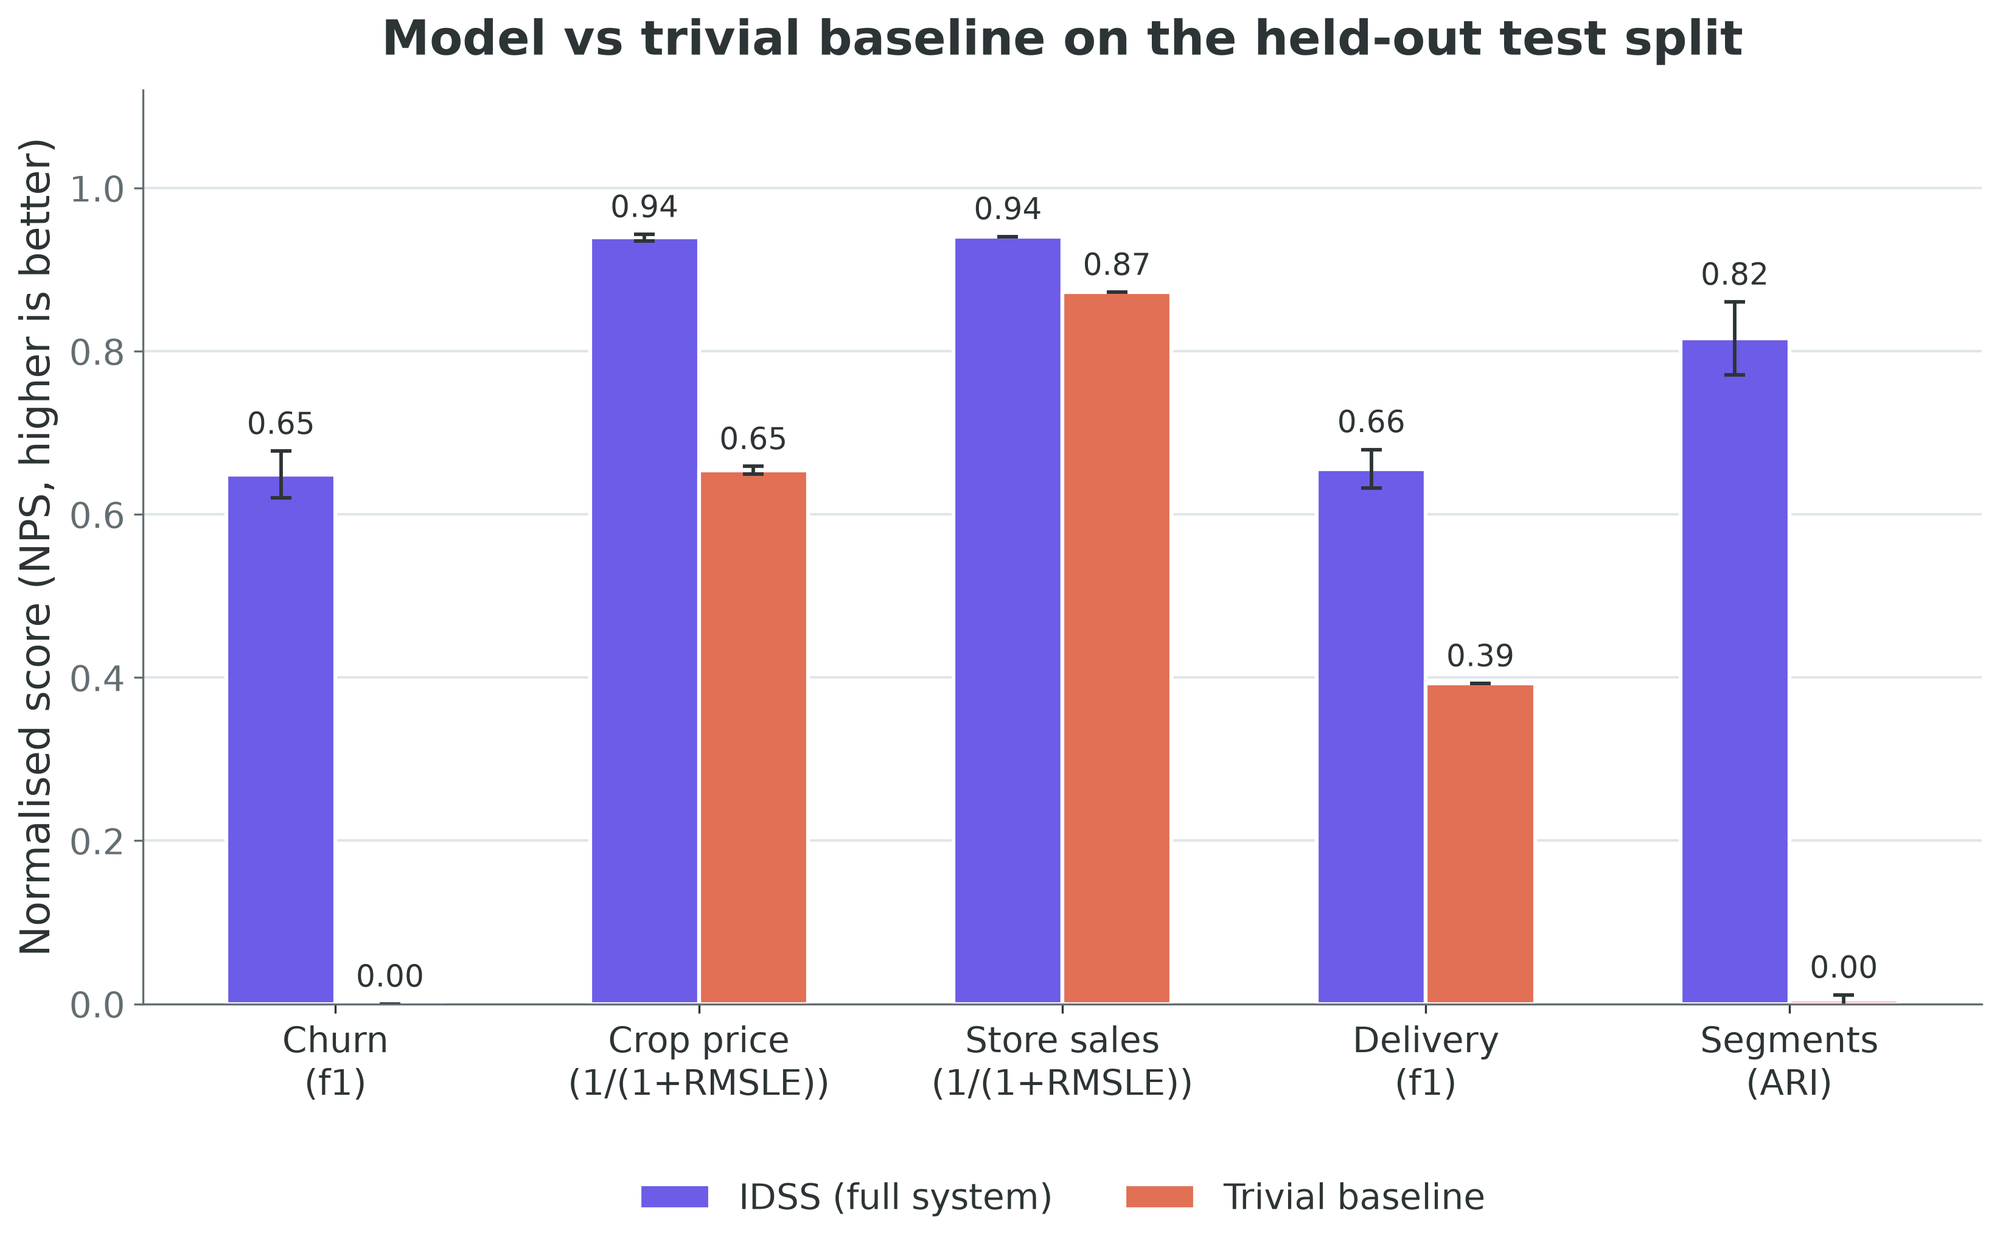
\includegraphics[width=\linewidth,height=7.3in,keepaspectratio]{figures/benchmark_vs_baseline.png}
  \caption{Model versus trivial baseline on the held-out test split (normalised score)}\label{fig:7.1}
\end{figure}

\FloatBarrier
\section{Paper-style Metrics: SR, NPS and CS}\label{sec:7.3}

Following AutoML-Agent \cite{ref9}:

\begin{quote}
\textbf{SR} = runs that complete the whole pipeline (trained, tested, verified, explained, PDF report) \ensuremath{\div} all runs; \textbf{NPS} = the test score for 0--1 metrics (F1; ARI clipped at 0), or 1 / (1 + RMSLE) for regression and forecasting, and 0 for a failed run; \textbf{CS} = 0.5 \ensuremath{\cdot} SR + 0.5 \ensuremath{\cdot} NPS.
\end{quote}

RMSLE = \ensuremath{\surd}( (1/\textit{n}) \ensuremath{\Sigma} (log(1 + \textit{\ensuremath{\hat{y}}}) \ensuremath{-} log(1 + \textit{y}))\textsuperscript{2} ) is scale-free; 1 / (1 + RMSE) would depend on the units of the target and be close to 0 for prices or daily sales. The overall value is the mean over datasets per seed, then over seeds.

\begin{table}[H]
\centering
\linespread{1}\small
\setlength{\tabcolsep}{4pt}
\caption{SR, NPS and CS (mean \ensuremath{\pm}~std over 3 seeds)}\label{tab:7.3}
\begin{tabular}{|>{\raggedright\arraybackslash\hspace{0pt}}p{\dimexpr 0.1783\linewidth-2\tabcolsep-2\arrayrulewidth\relax}|>{\raggedright\arraybackslash\hspace{0pt}}p{\dimexpr 0.2248\linewidth-2\tabcolsep-2\arrayrulewidth\relax}|>{\raggedleft\arraybackslash\hspace{0pt}}p{\dimexpr 0.1989\linewidth-2\tabcolsep-2\arrayrulewidth\relax}|>{\raggedleft\arraybackslash\hspace{0pt}}p{\dimexpr 0.1989\linewidth-2\tabcolsep-2\arrayrulewidth\relax}|>{\raggedleft\arraybackslash\hspace{0pt}}p{\dimexpr 0.1989\linewidth-2\tabcolsep-2\arrayrulewidth\relax}|}
\hline
\rowcolor{tableheader}\textbf{Dataset} & \textbf{NPS from} & \textbf{SR} & \textbf{NPS} & \textbf{CS} \\
\hline
Churn & F1 & 1.000 \ensuremath{\pm}~0.000 & 0.649 \ensuremath{\pm}~0.028 & 0.825 \ensuremath{\pm}~0.014 \\ \hline
Crop price & 1 / (1 + RMSLE) & 1.000 \ensuremath{\pm}~0.000 & 0.939 \ensuremath{\pm}~0.004 & 0.970 \ensuremath{\pm}~0.002 \\ \hline
Store sales & 1 / (1 + RMSLE) & 1.000 \ensuremath{\pm}~0.000 & 0.941 \ensuremath{\pm}~0.000 & 0.970 \ensuremath{\pm}~0.000 \\ \hline
Delivery & F1 & 1.000 \ensuremath{\pm}~0.000 & 0.656 \ensuremath{\pm}~0.024 & 0.828 \ensuremath{\pm}~0.012 \\ \hline
Segments & ARI & 1.000 \ensuremath{\pm}~0.000 & 0.816 \ensuremath{\pm}~0.045 & 0.908 \ensuremath{\pm}~0.022 \\ \hline
\textbf{Overall} &  & \textbf{1.000 \ensuremath{\pm}~0.000} & \textbf{0.800 \ensuremath{\pm}~0.011} & \textbf{0.900 \ensuremath{\pm}~0.005} \\ \hline
\end{tabular}
\end{table}

\begin{figure}[htbp]
  \centering
  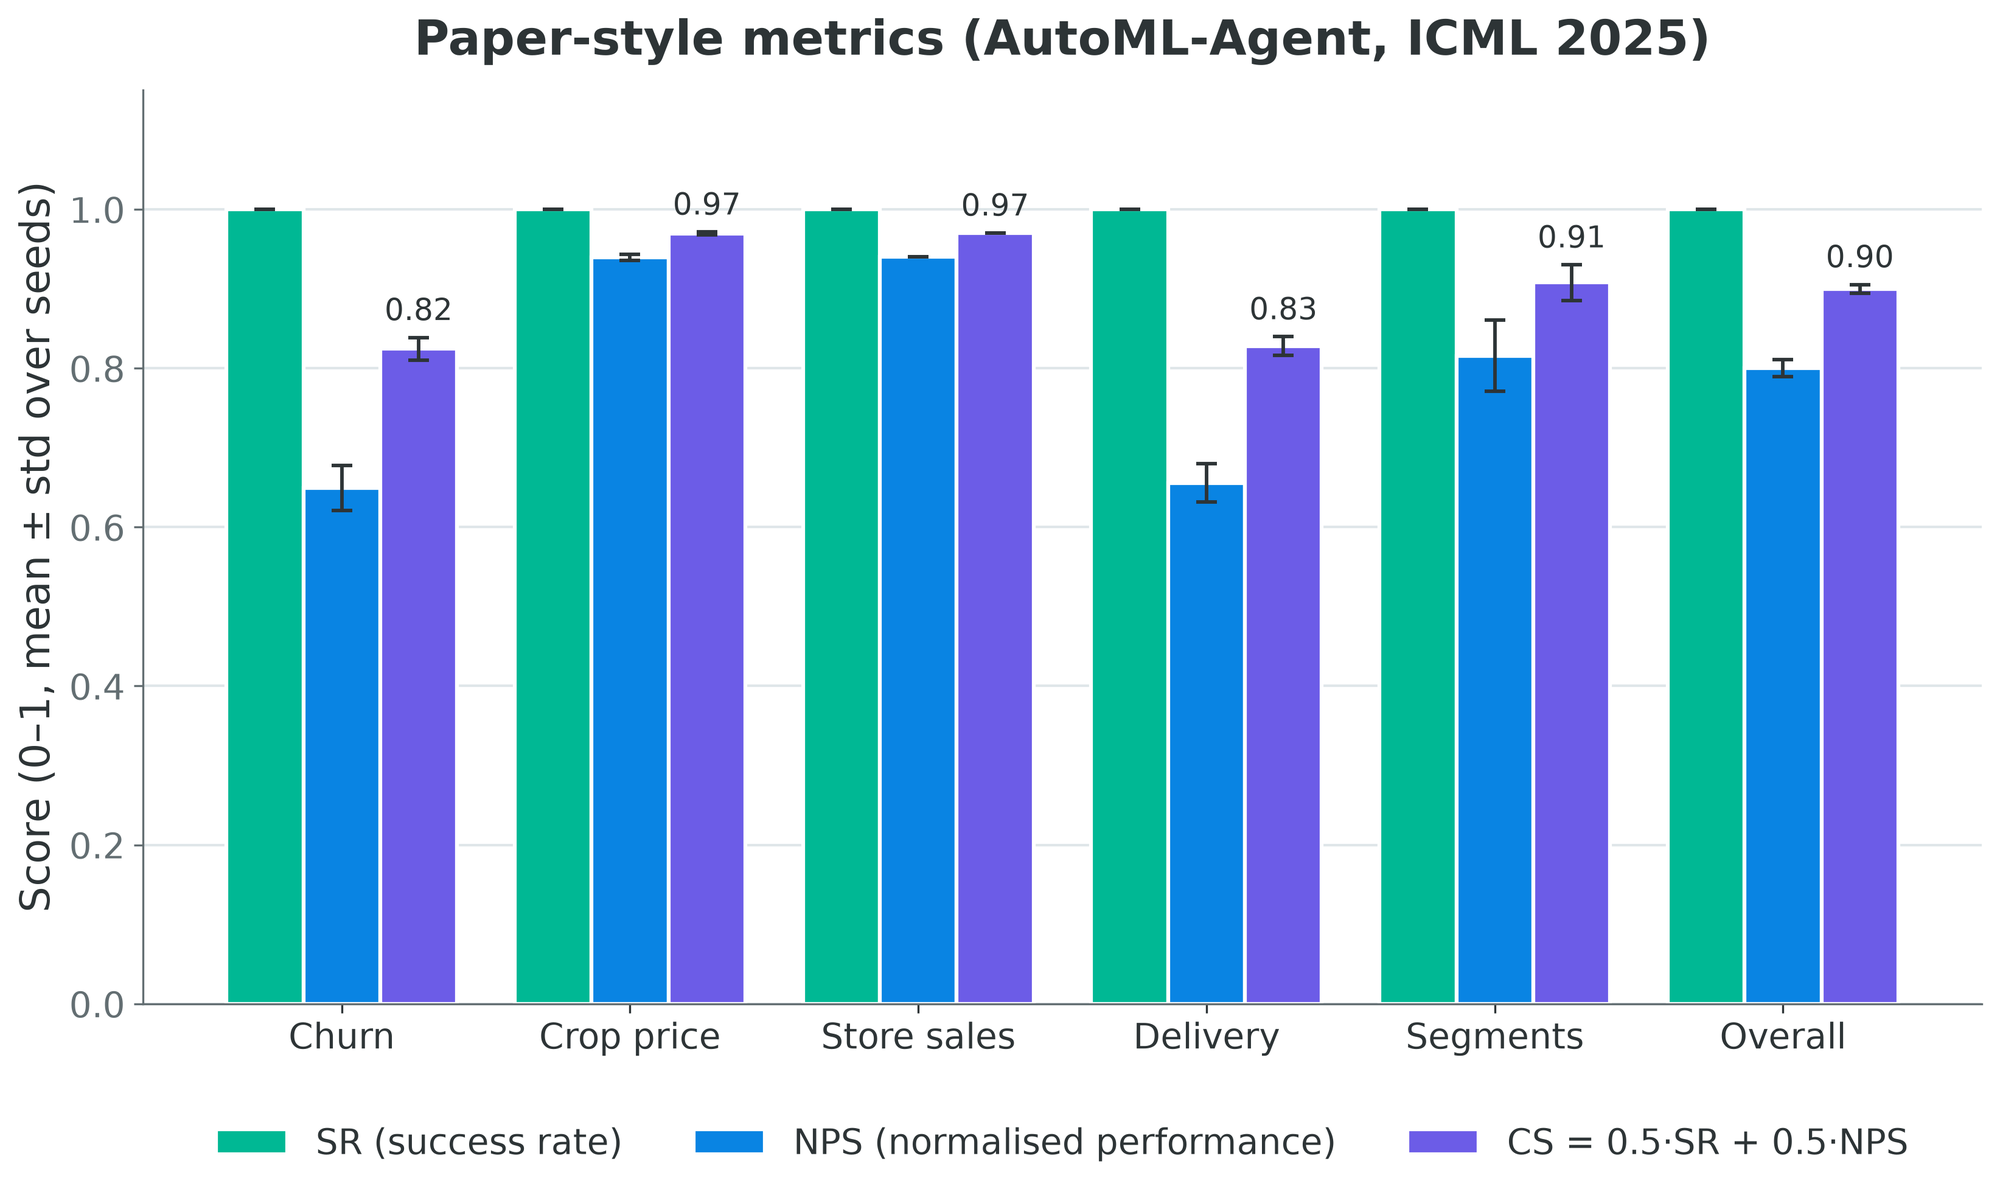
\includegraphics[width=\linewidth,height=7.3in,keepaspectratio]{figures/paper_metrics.png}
  \caption{Paper-style metrics (SR, NPS, CS) per dataset}\label{fig:7.2}
\end{figure}

All 15 runs completed end to end (SR = 1.00). Because IDSS runs tested code instead of LLM-written scripts, every run that starts also finishes, so SR measures robustness rather than code quality, and NPS carries the differences. \textbf{These numbers cannot be compared with the AutoML-Agent paper's tables}: datasets, budgets and success criteria differ.

\FloatBarrier
\section{Ablation Study}\label{sec:7.4}

One component was removed at a time: \textbf{\ensuremath{-} threshold tuning} (cut-off fixed at 0.5), \textbf{\ensuremath{-} hyperparameter tuning} (library defaults), \textbf{\ensuremath{-} verification re-planning} (first attempt is final) and a \textbf{single-model baseline} (one default LightGBM, or k-means for clustering, with none of the above). Ablation runs stop after verification. Table~\ref{tab:7.4} shows the test score and, in brackets, the change against the full system on the same seed (positive = better).

\begin{table}[H]
\centering
\linespread{1}\fontsize{9}{11}\selectfont
\setlength{\tabcolsep}{3pt}
\caption{Ablation study (mean \ensuremath{\pm}~std over 3 seeds)}\label{tab:7.4}
\begin{tabular}{|>{\raggedright\arraybackslash\hspace{0pt}}p{\dimexpr 0.1796\linewidth-2\tabcolsep-2\arrayrulewidth\relax}|>{\raggedleft\arraybackslash\hspace{0pt}}p{\dimexpr 0.1159\linewidth-2\tabcolsep-2\arrayrulewidth\relax}|>{\raggedleft\arraybackslash\hspace{0pt}}p{\dimexpr 0.1052\linewidth-2\tabcolsep-2\arrayrulewidth\relax}|>{\raggedleft\arraybackslash\hspace{0pt}}p{\dimexpr 0.1159\linewidth-2\tabcolsep-2\arrayrulewidth\relax}|>{\raggedleft\arraybackslash\hspace{0pt}}p{\dimexpr 0.1159\linewidth-2\tabcolsep-2\arrayrulewidth\relax}|>{\raggedleft\arraybackslash\hspace{0pt}}p{\dimexpr 0.1159\linewidth-2\tabcolsep-2\arrayrulewidth\relax}|>{\raggedleft\arraybackslash\hspace{0pt}}p{\dimexpr 0.0840\linewidth-2\tabcolsep-2\arrayrulewidth\relax}|>{\raggedleft\arraybackslash\hspace{0pt}}p{\dimexpr 0.0840\linewidth-2\tabcolsep-2\arrayrulewidth\relax}|>{\raggedleft\arraybackslash\hspace{0pt}}p{\dimexpr 0.0839\linewidth-2\tabcolsep-2\arrayrulewidth\relax}|}
\hline
\rowcolor{tableheader}\textbf{Variant} & \textbf{Churn (F1)} & \textbf{Crop price (RMSE)} & \textbf{Store sales (RMSE)} & \textbf{Delivery (F1)} & \textbf{Segments (ARI)} & \textbf{NPS} & \textbf{CS} & \textbf{Train time (s)} \\
\hline
\textbf{Full system} & 0.649 \ensuremath{\pm}~0.028 & 356.9 \ensuremath{\pm}~26.81 & 923.6 \ensuremath{\pm}~0.000 & 0.656 \ensuremath{\pm}~0.024 & 0.816 \ensuremath{\pm}~0.045 & 0.800 \ensuremath{\pm}~0.011 & \textbf{0.900 \ensuremath{\pm}~0.005} & 21.2 \ensuremath{\pm}~39.0 \\ \hline
\ensuremath{-} threshold tuning & 0.561 \ensuremath{\pm}~0.006 (\ensuremath{-}13.4\%) & same\textsuperscript{2} & same\textsuperscript{2} & same\textsuperscript{2} & same\textsuperscript{2} & 0.782 \ensuremath{\pm}~0.005 & 0.891 \ensuremath{\pm}~0.003 & 26.3 \ensuremath{\pm}~43.5 \\ \hline
\ensuremath{-} hyperparameter tuning & 0.648 \ensuremath{\pm}~0.027 (\ensuremath{-}0.1\%) & 378.5 \ensuremath{\pm}~52.63 (\ensuremath{-}5.7\%) & 915.7 \ensuremath{\pm}~0.000 (+0.9\%) & 0.669 \ensuremath{\pm}~0.021 (+2.0\%) & 0.523 \ensuremath{\pm}~0.078 (\ensuremath{-}35.6\%) & 0.743 \ensuremath{\pm}~0.018 & 0.871 \ensuremath{\pm}~0.009 & 1.9 \ensuremath{\pm}~1.5 \\ \hline
\ensuremath{-} verification re-planning & 0.649 \ensuremath{\pm}~0.028 (+0.0\%) & 356.9 \ensuremath{\pm}~26.81 (+0.0\%) & 923.6 \ensuremath{\pm}~0.000 (+0.0\%) & 0.656 \ensuremath{\pm}~0.024 (+0.0\%) & 0.816 \ensuremath{\pm}~0.045 (+0.0\%) & 0.800 \ensuremath{\pm}~0.011 & 0.900 \ensuremath{\pm}~0.005 & 12.8 \ensuremath{\pm}~11.0 \\ \hline
Single-model baseline & 0.521 \ensuremath{\pm}~0.057 (\ensuremath{-}19.3\%) & 368.4 \ensuremath{\pm}~41.67 (\ensuremath{-}3.0\%) & 1,298.8 \ensuremath{\pm}~0.000 (\ensuremath{-}40.6\%) & 0.648 \ensuremath{\pm}~0.020 (\ensuremath{-}1.1\%) & 0.508 \ensuremath{\pm}~0.012 (\ensuremath{-}37.6\%) & 0.707 \ensuremath{\pm}~0.016 & 0.854 \ensuremath{\pm}~0.008 & 0.7 \ensuremath{\pm}~0.4 \\ \hline
\end{tabular}
\end{table}

SR was 1.000 for every variant. \textsuperscript{2} Threshold tuning applies only to binary classification; the other datasets reuse the full-system runs.

\begin{figure}[htbp]
  \centering
  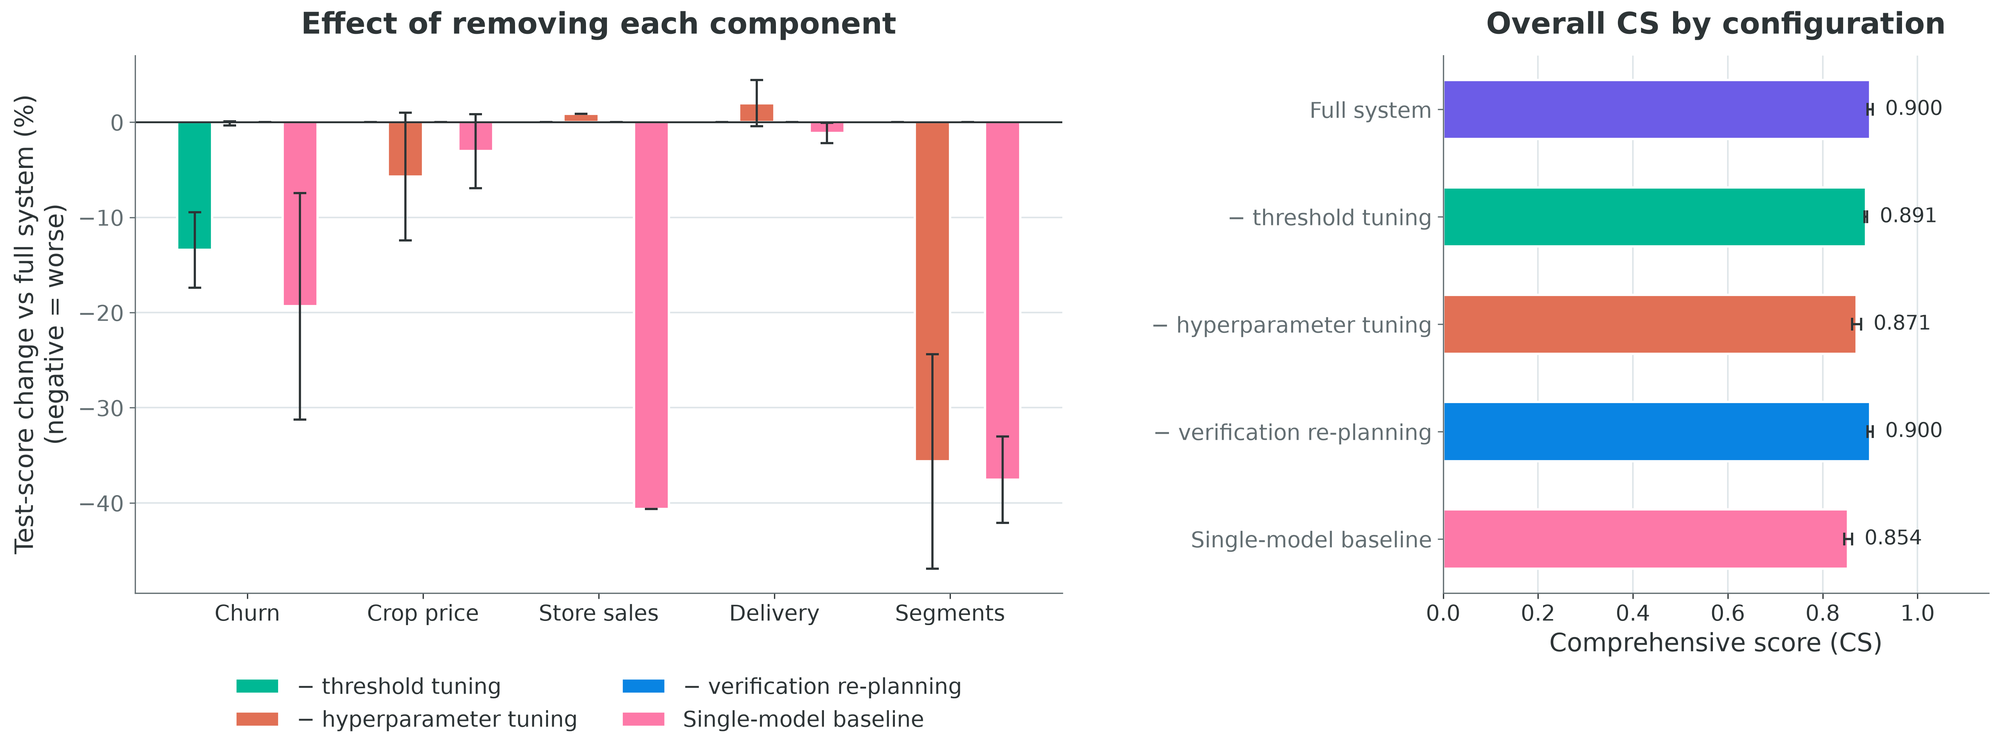
\includegraphics[width=\linewidth,height=7.3in,keepaspectratio]{figures/ablation.png}
  \caption{Ablation study: change of the test score per component and overall CS}\label{fig:7.3}
\end{figure}

\begin{itemize}
  \item \textbf{Threshold tuning} matters only for binary classification, but there it matters a lot: \ensuremath{-}13.4\% F1 on churn without it (Section~\ref{sec:7.6}).
  \item \textbf{Hyperparameter tuning} raises CS from 0.871 to 0.900. Without it, Segments loses 35.6\% (tuning finds the right number of clusters), while Delivery gains 2.0\%; where defaults scored higher on the test split, tuning had still chosen the best model on the validation split, a difference within selection noise on near-linear data.
  \item \textbf{Verification re-planning} was triggered in 1 of 15 clean full-system runs and did not change the score. Across all configurations it ran three times and the second attempt never passed; the system then reports \textit{not verified} (Section~\ref{sec:7.9}).
  \item \textbf{The single default model} reaches CS = 0.854 against 0.900 and passes verification in only 6 of 15 runs (full system: 14 of 15), with the largest losses on store sales (\ensuremath{-}40.6\%), segments (\ensuremath{-}37.6\%) and churn (\ensuremath{-}19.3\%).
\end{itemize}

\FloatBarrier
\section{Robustness}\label{sec:7.5}

The full system was re-run on corrupted copies of each dataset: \textbf{+10\% missing values} (cells blanked at random in all columns except the target, identifiers and the time index) and \textbf{+5 noisy columns} (three numeric, one integer, one categorical).

\begin{table}[H]
\centering
\linespread{1}\footnotesize
\setlength{\tabcolsep}{4pt}
\caption{Robustness (mean \ensuremath{\pm}~std over 3 seeds; change vs clean data, negative = worse)}\label{tab:7.5}
\begin{tabular}{|>{\raggedright\arraybackslash\hspace{0pt}}p{\dimexpr 0.1359\linewidth-2\tabcolsep-2\arrayrulewidth\relax}|>{\raggedright\arraybackslash\hspace{0pt}}p{\dimexpr 0.1067\linewidth-2\tabcolsep-2\arrayrulewidth\relax}|>{\raggedleft\arraybackslash\hspace{0pt}}p{\dimexpr 0.1059\linewidth-2\tabcolsep-2\arrayrulewidth\relax}|>{\raggedleft\arraybackslash\hspace{0pt}}p{\dimexpr 0.1307\linewidth-2\tabcolsep-2\arrayrulewidth\relax}|>{\raggedleft\arraybackslash\hspace{0pt}}p{\dimexpr 0.1169\linewidth-2\tabcolsep-2\arrayrulewidth\relax}|>{\raggedleft\arraybackslash\hspace{0pt}}p{\dimexpr 0.1322\linewidth-2\tabcolsep-2\arrayrulewidth\relax}|>{\raggedleft\arraybackslash\hspace{0pt}}p{\dimexpr 0.1139\linewidth-2\tabcolsep-2\arrayrulewidth\relax}|>{\raggedleft\arraybackslash\hspace{0pt}}p{\dimexpr 0.1577\linewidth-2\tabcolsep-2\arrayrulewidth\relax}|}
\hline
\rowcolor{tableheader}\textbf{Dataset} & \textbf{Metric} & \textbf{Clean} & \textbf{+10\% missing} & \textbf{Change} & \textbf{+5 noisy columns} & \textbf{Change} & \textbf{Verified (missing / noise)} \\
\hline
Churn & F1 \ensuremath{\uparrow} & 0.649 \ensuremath{\pm}~0.028 & 0.623 \ensuremath{\pm}~0.029 & \ensuremath{-}4.0\% \ensuremath{\pm}~1.2 & 0.644 \ensuremath{\pm}~0.036 & \ensuremath{-}0.9\% \ensuremath{\pm}~1.5 & 3/3 / 3/3 \\ \hline
Crop price & RMSE \ensuremath{\downarrow} & 356.9 \ensuremath{\pm}~26.81 & 562.9 \ensuremath{\pm}~95.98 & \ensuremath{-}57.1\% \ensuremath{\pm}~16.8 & 349.5 \ensuremath{\pm}~22.56 & +2.0\% \ensuremath{\pm}~1.1 & 3/3 / 3/3 \\ \hline
Store sales & RMSE \ensuremath{\downarrow} & 923.6 \ensuremath{\pm}~0.000 & 1,132.9 \ensuremath{\pm}~97.31 & \ensuremath{-}22.7\% \ensuremath{\pm}~10.5 & 938.5 \ensuremath{\pm}~15.17 & \ensuremath{-}1.6\% \ensuremath{\pm}~1.6 & 3/3 / 3/3 \\ \hline
Delivery & F1 \ensuremath{\uparrow} & 0.656 \ensuremath{\pm}~0.024 & 0.613 \ensuremath{\pm}~0.011 & \ensuremath{-}6.5\% \ensuremath{\pm}~1.7 & 0.659 \ensuremath{\pm}~0.024 & +0.5\% \ensuremath{\pm}~2.3 & 2/3 / 3/3 \\ \hline
Segments & ARI \ensuremath{\uparrow} & 0.816 \ensuremath{\pm}~0.045 & 0.729 \ensuremath{\pm}~0.042 & \ensuremath{-}10.6\% \ensuremath{\pm}~0.3 & 0.833 \ensuremath{\pm}~0.053 & +2.2\% \ensuremath{\pm}~5.9 & 3/3 / 3/3 \\ \hline
\end{tabular}
\end{table}

\begin{figure}[htbp]
  \centering
  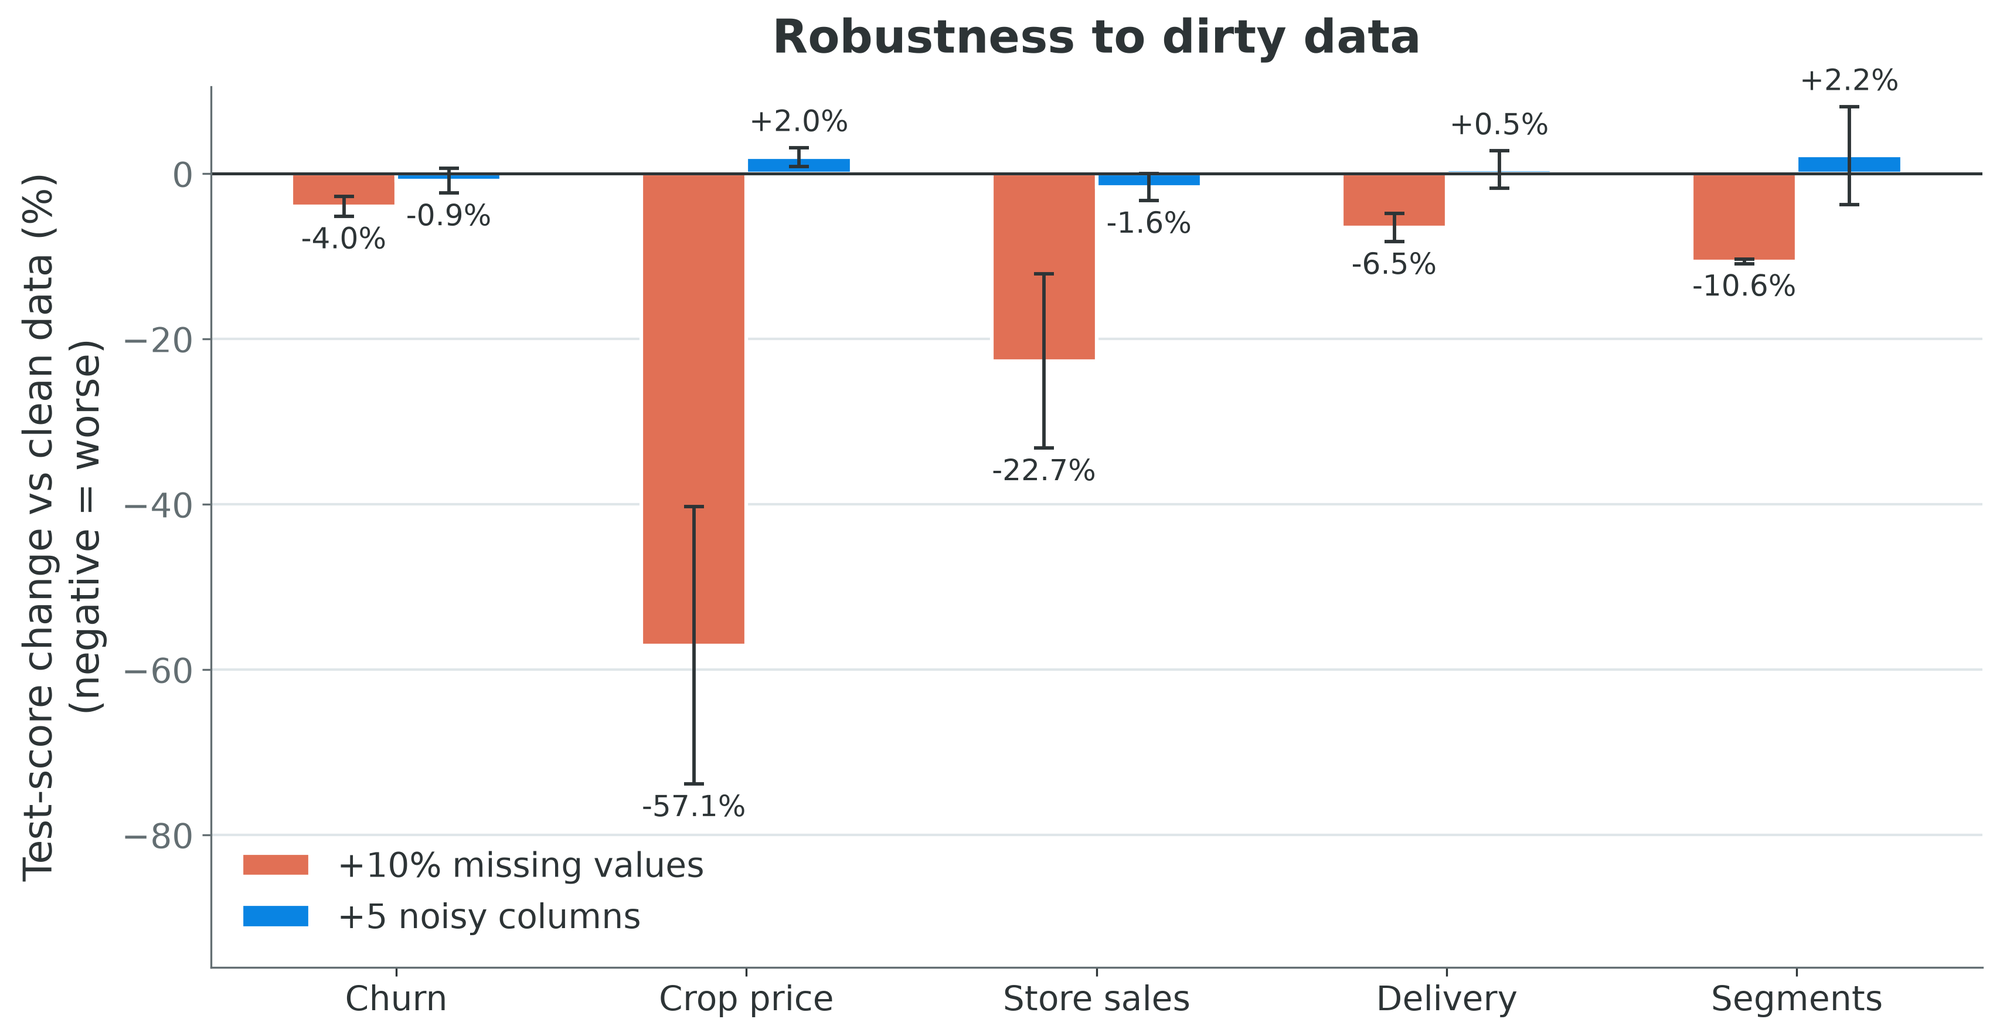
\includegraphics[width=\linewidth,height=7.3in,keepaspectratio]{figures/robustness.png}
  \caption{Robustness: change of the test score with 10\% extra missing values and with 5 noisy columns}\label{fig:7.4}
\end{figure}

Noise columns changed every score by at most 2.2\%: irrelevant features did not mislead the models. Missing values hurt more: 6 of the 10 perturbed settings stayed within 5\% of the clean score, and the largest losses were crop price (RMSE +57.1\%) and store sales (+22.7\%), plausibly because the simple imputation cannot recover the blanked information. Verification still passed in 29 of the 30 perturbed runs.

\FloatBarrier
\section{Impact of Threshold Tuning on Churn}\label{sec:7.6}

Churners are the minority (32.8\%), so a 0.5 cut-off is conservative and misses many of them. Over the three seeds, threshold tuning raises churn F1 from 0.561 \ensuremath{\pm}~0.006 (cut-off 0.5) to 0.649 \ensuremath{\pm}~0.028, a change of \ensuremath{-}13.4\% when it is removed (Table~\ref{tab:7.4}). Table~\ref{tab:7.6} shows the effect in more detail for a single demo run (seed 42): the selected logistic regression on the seed-42 split (Step 5 benchmark).

\begin{table}[H]
\centering
\linespread{1}\small
\setlength{\tabcolsep}{4pt}
\caption{Threshold tuning on churn (single demo run, seed 42: logistic regression, test split)}\label{tab:7.6}
\begin{tabular}{|>{\raggedright\arraybackslash\hspace{0pt}}p{\dimexpr 0.4386\linewidth-2\tabcolsep-2\arrayrulewidth\relax}|>{\raggedleft\arraybackslash\hspace{0pt}}p{\dimexpr 0.2225\linewidth-2\tabcolsep-2\arrayrulewidth\relax}|>{\raggedleft\arraybackslash\hspace{0pt}}p{\dimexpr 0.3389\linewidth-2\tabcolsep-2\arrayrulewidth\relax}|}
\hline
\rowcolor{tableheader}\textbf{Metric} & \textbf{Cut-off 0.5} & \textbf{Tuned cut-off 0.32} \\
\hline
F1 & 0.5579 & 0.6230 \\ \hline
Precision & 0.5824 & 0.5241 \\ \hline
Recall & 0.5354 & 0.7677 \\ \hline
Accuracy & 0.7200 & 0.6933 \\ \hline
ROC AUC (threshold-free) & 0.7738 & 0.7738 \\ \hline
\end{tabular}
\end{table}

The tuned cut-off \textbf{trades a little precision and accuracy for much higher recall}: in this run about 77\% of churners are found instead of 54\%, usually the right trade-off for a retention campaign. Over the three seeds the tuned thresholds were 0.32, 0.36 and 0.23.

The cut-off also drives the \textbf{risk tiers} (Figure~\ref{fig:5.5}; the same single demo run, seed 42, scored on all 3,000 customers). High risk starts at a probability of 0.4609 --- the larger of the threshold 0.32 and the 70th percentile --- and holds 900 customers (30.0\%); Medium (0.32 to 0.4609) holds 447 (14.9\%) and Low 1,653 (55.1\%). The strongest drivers were \code{contract\_\allowbreak{}type} (34\% of the explanation), \code{tenure\_\allowbreak{}months} (20\%) and \code{payment\_\allowbreak{}method} (13\%). Moving the high-risk customers to a two-year contract would lower their average predicted churn probability from 0.651 to 0.193 according to the model --- a statement about the model, not a guaranteed effect of a campaign.

\FloatBarrier
\section{Clustering: Adjusted Rand Index versus Rand Index}\label{sec:7.7}

AutoML-Agent scores clustering with the Rand index (RI) \cite{ref17}, the share of record pairs on which clustering and ground truth agree. Because most pairs belong to different groups, RI rewards over-splitting and is not corrected for chance: a random assignment into four groups already scores about 0.62 here, and in a first run an untuned k-means with 8 clusters beat the tuned 4-cluster model on RI. The \textbf{adjusted Rand index} \cite{ref18}, ARI = (RI \ensuremath{-} E[RI]) / (max(RI) \ensuremath{-} E[RI]), scores about 0 for random labels and 1 for a perfect match. IDSS therefore uses ARI wherever ground truth exists and still reports RI (Table~\ref{tab:7.7}).

The investigation also exposed a bug: the Gaussian mixture ran a single EM initialisation and, for some seeds, its refit stopped in a poor optimum (ARI \ensuremath{\approx} 0.53 instead of 0.84), which made added noise look like an improvement. It now uses several initialisations (5, or 3 above 20,000 rows). Segments was re-run after both changes; the replaced runs are kept under \code{superseded} in \code{evaluation.json}.

\begin{table}[H]
\centering
\linespread{1}\small
\setlength{\tabcolsep}{4pt}
\caption{Clustering results with ARI and RI (Segments, mean \ensuremath{\pm}~std over 3 seeds)}\label{tab:7.7}
\begin{tabular}{|>{\raggedright\arraybackslash\hspace{0pt}}p{\dimexpr 0.3248\linewidth-2\tabcolsep-2\arrayrulewidth\relax}|>{\raggedright\arraybackslash\hspace{0pt}}p{\dimexpr 0.3656\linewidth-2\tabcolsep-2\arrayrulewidth\relax}|>{\raggedleft\arraybackslash\hspace{0pt}}p{\dimexpr 0.1548\linewidth-2\tabcolsep-2\arrayrulewidth\relax}|>{\raggedleft\arraybackslash\hspace{0pt}}p{\dimexpr 0.1548\linewidth-2\tabcolsep-2\arrayrulewidth\relax}|}
\hline
\rowcolor{tableheader}\textbf{Configuration} & \textbf{Models chosen} & \textbf{ARI \ensuremath{\uparrow}} & \textbf{RI \ensuremath{\uparrow}} \\
\hline
Full system & Gaussian mixture \ensuremath{\times} 3 & 0.816 \ensuremath{\pm}~0.045 & 0.930 \ensuremath{\pm}~0.017 \\ \hline
\ensuremath{-} hyperparameter tuning & agglomerative \ensuremath{\times} 2, k-means & 0.523 \ensuremath{\pm}~0.078 & 0.804 \ensuremath{\pm}~0.046 \\ \hline
Single-model baseline & k-means \ensuremath{\times} 3 & 0.508 \ensuremath{\pm}~0.012 & 0.841 \ensuremath{\pm}~0.006 \\ \hline
Full system, +10\% missing & agglomerative, Gaussian mixture \ensuremath{\times} 2 & 0.729 \ensuremath{\pm}~0.042 & 0.896 \ensuremath{\pm}~0.014 \\ \hline
Full system, +5 noisy columns & Gaussian mixture \ensuremath{\times} 3 & 0.833 \ensuremath{\pm}~0.053 & 0.936 \ensuremath{\pm}~0.019 \\ \hline
\end{tabular}
\end{table}

The random baseline scored RI = 0.625 but ARI = 0.004, which shows why the chance-corrected index is fairer.

\FloatBarrier
\section{Efficiency}\label{sec:7.8}

With the fast budget the search plus refit took 2.7 s (Segments) to 19.8 s (Churn) on average; Delivery averaged 72.2 s with a wide spread because one seed triggered a full-budget re-plan (157.9 s). Inference took 0.016 to 0.201 ms per row, preprocessing included; the time-series pipeline is the slowest per row, probably because it builds lag and rolling features at prediction time (Figure~\ref{fig:7.5}).

\begin{figure}[htbp]
  \centering
  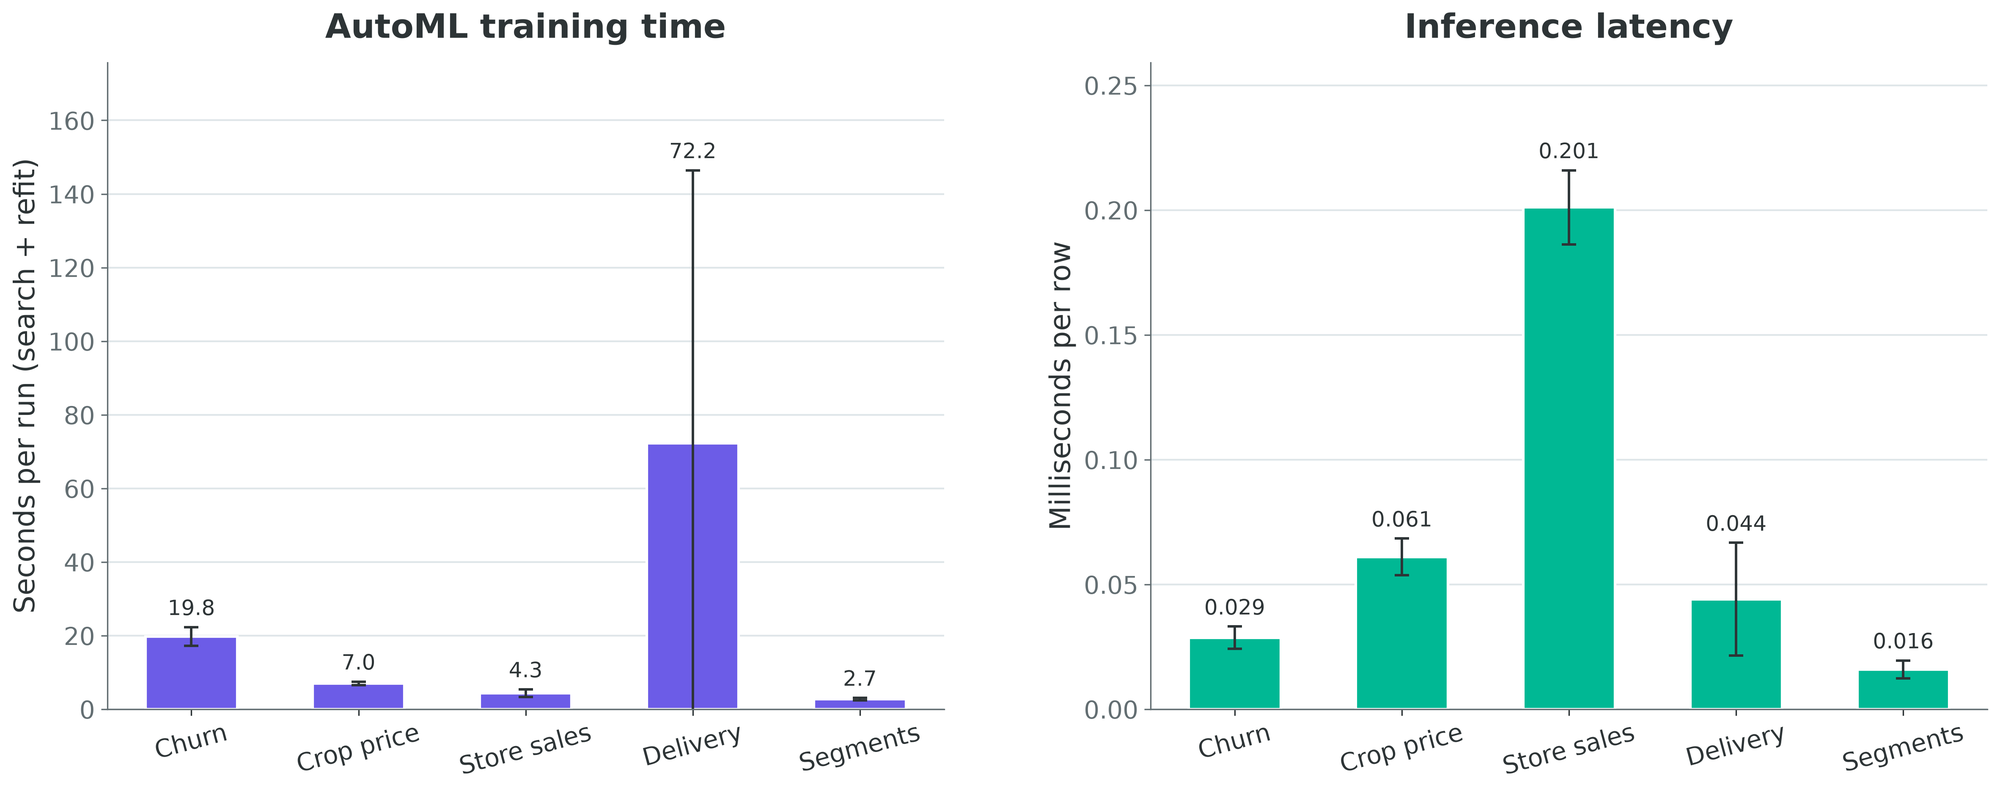
\includegraphics[width=\linewidth,height=7.3in,keepaspectratio]{figures/efficiency.png}
  \caption{Efficiency: AutoML training time per run and inference latency per row}\label{fig:7.5}
\end{figure}

\FloatBarrier
\section{Verification Outcomes}\label{sec:7.9}

Verification passed in 14 of 15 clean full-system runs. Table~\ref{tab:7.8} lists the full-system and variant runs that did not pass; all failed the overfitting check (train--test gap \ensuremath{\geq} 0.15 on the primary 0--1 metric).

\begin{table}[H]
\centering
\linespread{1}\footnotesize
\setlength{\tabcolsep}{4pt}
\caption{Runs that did not pass verification}\label{tab:7.8}
\begin{tabular}{|>{\raggedright\arraybackslash\hspace{0pt}}p{\dimexpr 0.1315\linewidth-2\tabcolsep-2\arrayrulewidth\relax}|>{\raggedleft\arraybackslash\hspace{0pt}}p{\dimexpr 0.0820\linewidth-2\tabcolsep-2\arrayrulewidth\relax}|>{\raggedright\arraybackslash\hspace{0pt}}p{\dimexpr 0.2114\linewidth-2\tabcolsep-2\arrayrulewidth\relax}|>{\raggedright\arraybackslash\hspace{0pt}}p{\dimexpr 0.1405\linewidth-2\tabcolsep-2\arrayrulewidth\relax}|>{\raggedleft\arraybackslash\hspace{0pt}}p{\dimexpr 0.0974\linewidth-2\tabcolsep-2\arrayrulewidth\relax}|>{\raggedright\arraybackslash\hspace{0pt}}p{\dimexpr 0.1563\linewidth-2\tabcolsep-2\arrayrulewidth\relax}|>{\raggedright\arraybackslash\hspace{0pt}}p{\dimexpr 0.1809\linewidth-2\tabcolsep-2\arrayrulewidth\relax}|}
\hline
\rowcolor{tableheader}\textbf{Dataset} & \textbf{Seed} & \textbf{Configuration} & \textbf{Selected model} & \textbf{Test F1} & \textbf{Re-planned} & \textbf{Outcome} \\
\hline
Delivery & 44 & Full system, clean & LightGBM & 0.636 & Yes & Still failing; DONE, flagged \textit{not verified} \\ \hline
Delivery & 42 & Full system, +10\% missing & XGBoost & 0.625 & Yes & Still failing; flagged \textit{not verified} \\ \hline
Churn & 43 & \ensuremath{-} threshold tuning & LightGBM & 0.568 & Yes & Still failing; flagged \textit{not verified} \\ \hline
\end{tabular}
\end{table}

The single default LightGBM failed the same check in 9 of 15 runs (Churn, Store sales and Delivery on every seed). These cases show the verifier working as intended: when a boosted-tree model fitted the training rows much better than the test rows and the full-budget re-plan could not fix it, the system completed the analysis but labelled the result \textit{not verified} instead of presenting an over-fitted model as trustworthy.

\FloatBarrier
\section{Discussion}\label{sec:7.10}

\textbf{Strengths.}

\begin{itemize}
  \item \textbf{Every run finishes} (SR = 1.00) because the LLM plans but never writes training code.
  \item \textbf{Better than trivial on every dataset}, with RMSE reductions of 85.1\% and 60.5\% and an ARI of 0.816 against about 0.
  \item \textbf{Each component contributes}: search, tuning and threshold tuning raise CS from 0.854 to 0.900, and threshold tuning alone raises F1 on the imbalanced churn data from 0.561 to 0.649 (\ensuremath{-}13.4\% without it).
  \item \textbf{Robust to irrelevant features}: five noise columns changed scores by at most 2.2\%.
  \item \textbf{Honest self-assessment}: the test split was read once in every run, baselines used the same split, over-fitting was reported rather than hidden, and the evaluation itself caught a misleading metric and an engine bug.
  \item \textbf{Decisions, not only scores}: risk tiers with stated cut-offs, drivers and actions with expected effects, and a brief whose numbers are grounded in computed facts.
\end{itemize}

\textbf{Limitations.}

\begin{itemize}
  \item \textbf{Synthetic data}: real business data is noisier and may contain drift, label noise or leakage, so these results are not performance on real data.
  \item \textbf{The LLM path is not benchmarked}: the evaluation ran offline, so parsing, the knowledge brief, the LLM review and the written insights used their fallbacks; the results measure the engine and the pipeline.
  \item \textbf{Small study}: three seeds, the fast budget and one machine.
  \item \textbf{Missing values} are the main weakness (crop price RMSE +57.1\%), and on Delivery the single re-plan did not cure over-fitting; a different strategy on the second attempt would be needed.
  \item \textbf{Correlation, not causation}: drivers, what-if results and counterfactual actions describe the model's response, not real-world effects, which only an experiment can measure.
\end{itemize}

\FloatBarrier
\section{Summary}\label{sec:7.11}

On five synthetic, seeded datasets IDSS completed every run (SR = 1.00) with NPS = 0.800 and CS = 0.900, beat the baseline everywhere and passed verification in 14 of 15 full-system runs. The ablation showed the value of model search, tuning and especially threshold tuning; the robustness study showed that noise is harmless while missing values hurt; ARI made the clustering evaluation fair; and the verifier flagged over-fitted runs instead of hiding them.

% Generated by scripts/build_latex.py from docs/report/ch8_conclusion.md: edit the Markdown, not this file.
\chapter{Conclusion and Future Scope}\label{ch:8}

\FloatBarrier
\section{Conclusion}\label{sec:8.1}

We designed, built, tested and evaluated an \textbf{Intelligent Decision Support System (IDSS)} that turns a business question in plain language and a table of data into a verified machine-learning model and explained, actionable decisions. Inspired by AutoML-Agent \cite{ref9}, we kept its multi-agent decomposition, structured requirements, retrieval-augmented planning, multi-stage verification and evaluation metrics, and changed the division of labour so that \textbf{LLM agents plan and explain while deterministic, tested code computes every number}.

The objectives of Section~\ref{sec:1.3.2} were met:

\begin{enumerate}
  \item A resumable 13-state Orchestrator coordinates seven agents, each with a deterministic fallback, so the full pipeline runs without an LLM.
  \item The Requirement Agent checks relevance, parses and repairs the requirement against the data and asks at most two rounds of clarifying questions.
  \item The AutoML engine tunes a fixed scikit-learn / XGBoost / LightGBM zoo with Optuna within budgets and constraints, tunes the decision threshold and reads the test split exactly once, which is audited.
  \item Seven verification checks decide whether a result can be trusted, with one re-plan and an explicit \textit{not verified} label when the problem persists.
  \item SHAP drivers, what-if simulation, risk tiers, counterfactual actions and forecasts are combined in a grounded decision brief and PDF / Markdown reports.
  \item A 17-endpoint FastAPI backend and an eight-page Streamlit interface with Demo Mode make the system usable from a browser, and runs survive restarts.
  \item Only aggregates reach the LLM, keys stay in \code{.env}, LLM-written code runs only in a sandbox and all loops and retries are bounded.
  \item On five synthetic, seeded datasets the system completed every run (SR = 1.00) with NPS = 0.800 and CS = 0.900, beat the baseline everywhere and passed verification in 14 of 15 runs; 449 automated tests (447 offline, all passing) cover 93\% of the code.
\end{enumerate}

The project also taught us that honest evaluation changes a system: the Rand index proved misleading for clustering, so we adopted the adjusted Rand index \cite{ref18}, and the same investigation revealed and fixed a real bug; a small component, threshold tuning, mattered more on imbalanced data than hyperparameter tuning; and a verifier that may say ``not verified'' is more useful to a decision maker than one that always passes. IDSS has clear limits --- one table at a time, synthetic and offline evaluation, sensitivity to missing values and model-based rather than causal what-if results --- but within them it shows that LLM agents for language combined with deterministic engines for computation give a decision support system that is conversational, reproducible, self-checking and safe to run on a laptop.

\FloatBarrier
\section{Future Scope}\label{sec:8.2}

\begin{itemize}
  \item \textbf{Real-data studies:} public benchmark datasets and a partner organisation's data, with a user study of decision quality and time saved.
  \item \textbf{Benchmark the LLM path:} parsing accuracy, usefulness of clarifying questions, faithfulness of briefs and cost per run across several providers.
  \item \textbf{Stronger AutoML:} cross-validation for small data, ensembling, better imputation for missing values, more and multi-series forecasting models, calibrated prediction intervals.
  \item \textbf{Smarter re-planning:} change the strategy after a failed verification (regularisation, simpler models, more cleaning), not only the budget.
  \item \textbf{Causal and prescriptive decisions:} uplift modelling, cost-aware optimisation of actions, feasibility constraints in counterfactuals.
  \item \textbf{Multi-user deployment and model operations:} authentication, a job queue, containers, prediction services, drift monitoring and scheduled retraining.
  \item \textbf{Richer knowledge and explanations:} domain knowledge packs, embedding-based retrieval with cited passages, interactive explanations and reports in regional languages such as Marathi and Hindi.
\end{itemize}

\FloatBarrier
\section{Summary}\label{sec:8.3}

IDSS met its eight objectives: it understands a plain-language question, builds and verifies a model with deterministic code, turns it into explained, actionable decisions and delivers them through a safe, resumable web application that also works offline. The future work follows from its limitations --- real data, evaluation of the LLM path, robustness to missing data and causal decision support.

% References in the college style, numbered by first citation as in the Word report.
% Generated by scripts/build_latex.py from docs/report/references.md.
\begin{thebibliography}{99}
\frontentry{References}
\bibitem{ref1} D. J. Power, ``Decision Support Systems: Concepts and Resources for Managers'', \textit{Quorum Books (Greenwood Publishing Group), Westport, CT, USA, 2002.}

\bibitem{ref2} F. Pedregosa, G. Varoquaux, A. Gramfort, V. Michel, B. Thirion, O. Grisel, M. Blondel, P. Prettenhofer, R. Weiss, V. Dubourg, J. Vanderplas, A. Passos, D. Cournapeau, M. Brucher, M. Perrot and \'{E}. Duchesnay, ``Scikit-learn: Machine Learning in Python'', \textit{Journal of Machine Learning Research, vol. 12, 2011, pp. 2825--2830.}

\bibitem{ref3} T. Chen and C. Guestrin, ``XGBoost: A Scalable Tree Boosting System'', \textit{Proceedings of the 22nd ACM SIGKDD International Conference on Knowledge Discovery and Data Mining (KDD '16), ACM, San Francisco, CA, USA, 2016, pp. 785--794.}

\bibitem{ref4} G. Ke, Q. Meng, T. Finley, T. Wang, W. Chen, W. Ma, Q. Ye and T.-Y. Liu, ``LightGBM: A Highly Efficient Gradient Boosting Decision Tree'', \textit{Advances in Neural Information Processing Systems 30 (NIPS 2017), Curran Associates, Long Beach, CA, USA, 2017, pp. 3146--3154.}

\bibitem{ref5} M. Feurer, A. Klein, K. Eggensperger, J. T. Springenberg, M. Blum and F. Hutter, ``Efficient and Robust Automated Machine Learning'', \textit{Advances in Neural Information Processing Systems 28 (NIPS 2015), Curran Associates, Montr\'{e}al, Canada, 2015, pp. 2962--2970.}

\bibitem{ref6} J. Bergstra, R. Bardenet, Y. Bengio and B. K\'{e}gl, ``Algorithms for Hyper-Parameter Optimization'', \textit{Advances in Neural Information Processing Systems 24 (NIPS 2011), Curran Associates, Granada, Spain, 2011, pp. 2546--2554.}

\bibitem{ref7} T. Akiba, S. Sano, T. Yanase, T. Ohta and M. Koyama, ``Optuna: A Next-generation Hyperparameter Optimization Framework'', \textit{Proceedings of the 25th ACM SIGKDD International Conference on Knowledge Discovery \& Data Mining (KDD '19), ACM, Anchorage, AK, USA, 2019, pp. 2623--2631.}

\bibitem{ref8} S. Yao, J. Zhao, D. Yu, N. Du, I. Shafran, K. Narasimhan and Y. Cao, ``ReAct: Synergizing Reasoning and Acting in Language Models'', \textit{International Conference on Learning Representations (ICLR 2023), Kigali, Rwanda, 2023. \url{https://arxiv.org/abs/2210.03629}}

\bibitem{ref9} P. Trirat, W. Jeong and S. J. Hwang, ``AutoML-Agent: A Multi-Agent LLM Framework for Full-Pipeline AutoML'', \textit{Proceedings of the 42nd International Conference on Machine Learning (ICML 2025), PMLR, Vancouver, Canada, 2025. \url{https://arxiv.org/abs/2410.02958}}

\bibitem{ref10} S. M. Lundberg and S.-I. Lee, ``A Unified Approach to Interpreting Model Predictions'', \textit{Advances in Neural Information Processing Systems 30 (NIPS 2017), Curran Associates, Long Beach, CA, USA, 2017, pp. 4765--4774.}

\bibitem{ref11} S. Wachter, B. Mittelstadt and C. Russell, ``Counterfactual Explanations without Opening the Black Box: Automated Decisions and the GDPR'', \textit{Harvard Journal of Law \& Technology, vol. 31, no. 2, 2018, pp. 841--887 (preprint 2017). \url{https://arxiv.org/abs/1711.00399}}

\bibitem{ref12} Q. Wu, G. Bansal, J. Zhang, Y. Wu, B. Li, E. Zhu, L. Jiang, X. Zhang, S. Zhang, J. Liu, A. H. Awadallah, R. W. White, D. Burger and C. Wang, ``AutoGen: Enabling Next-Gen LLM Applications via Multi-Agent Conversation'', \textit{arXiv preprint arXiv:2308.08155, 2023. \url{https://arxiv.org/abs/2308.08155}}

\bibitem{ref13} S. Hong et al., ``Data Interpreter: An LLM Agent for Data Science'', \textit{arXiv preprint arXiv:2402.18679, 2024. \url{https://arxiv.org/abs/2402.18679}}

\bibitem{ref14} P. Lewis, E. Perez, A. Piktus, F. Petroni, V. Karpukhin, N. Goyal, H. K\"{u}ttler, M. Lewis, W. Yih, T. Rockt\"{a}schel, S. Riedel and D. Kiela, ``Retrieval-Augmented Generation for Knowledge-Intensive NLP Tasks'', \textit{Advances in Neural Information Processing Systems 33 (NeurIPS 2020), Curran Associates, 2020, pp. 9459--9474.}

\bibitem{ref15} M. T. Ribeiro, S. Singh and C. Guestrin, ``{}`Why Should I Trust You?': Explaining the Predictions of Any Classifier'', \textit{Proceedings of the 22nd ACM SIGKDD International Conference on Knowledge Discovery and Data Mining (KDD '16), ACM, San Francisco, CA, USA, 2016, pp. 1135--1144.}

\bibitem{ref16} B. W. Boehm, ``Software Engineering Economics'', \textit{Prentice-Hall, Englewood Cliffs, NJ, USA, 1981.}

\bibitem{ref17} W. M. Rand, ``Objective Criteria for the Evaluation of Clustering Methods'', \textit{Journal of the American Statistical Association, vol. 66, no. 336, 1971, pp. 846--850.}

\bibitem{ref18} L. Hubert and P. Arabie, ``Comparing Partitions'', \textit{Journal of Classification, Springer, vol. 2, no. 1, 1985, pp. 193--218.}

\end{thebibliography}

% Generated by scripts/build_latex.py from docs/report/publications.md.
\chapter*{Publications and Certificates}
\frontentry{Publications and Certificates}

\noindent Nil.

\appendix
% Generated by scripts/build_latex.py from docs/report/appendix_a_user_manual.md: edit the Markdown, not this file.
\chapter{User Manual (Short)}\label{ch:A}

This appendix summarises how to install and use IDSS. The full manual is \code{docs/\allowbreak{}user\_\allowbreak{}manual.\allowbreak{}md} in the repository.

\FloatBarrier
\section{Requirements}\label{sec:A.1}

\begin{itemize}
  \item Windows 10 or 11, Python 3.12 and Git; about 2 GB of free disk space for the virtual environment.
  \item Optional: an API key for an OpenAI-compatible LLM provider (OpenAI, Groq, Google Gemini) or a local Ollama model. Without one, everything except \textit{Ask Your Data} works in offline mode.
\end{itemize}

\FloatBarrier
\section{Installation}\label{sec:A.2}

From a PowerShell window in the project folder:

\begin{lstlisting}
python -m venv .venv
.venv\Scripts\python.exe -m pip install -r requirements.txt
Copy-Item .env.example .env
# optional check: the offline test suite
.venv\Scripts\python.exe -m pytest -q
\end{lstlisting}

To use an LLM, set \code{LLM\_\allowbreak{}PROVIDER}, \code{LLM\_\allowbreak{}MODEL} and \code{LLM\_\allowbreak{}API\_\allowbreak{}KEY} in \code{.env} (the file stays on the computer and is ignored by Git). Leave them empty for offline mode.

\FloatBarrier
\section{Starting and Stopping}\label{sec:A.3}

\begin{lstlisting}
powershell -ExecutionPolicy Bypass -File scripts\run_all.ps1
\end{lstlisting}

This starts the API (\code{http:/\allowbreak{}/\allowbreak{}localhost:8000}, interactive documentation at \code{/docs}) in a new window and then the user interface at \code{http:/\allowbreak{}/\allowbreak{}localhost:8501}. Stop the UI with Ctrl+C and close the API window to stop the backend. Both servers listen on this computer only.

\FloatBarrier
\section{Pages}\label{sec:A.4}

\begin{table}[H]
\centering
\linespread{1}\small
\setlength{\tabcolsep}{4pt}
\caption{Pages of the user interface}\label{tab:A.1}
\begin{tabular}{|>{\raggedright\arraybackslash\hspace{0pt}}p{\dimexpr 0.2128\linewidth-2\tabcolsep-2\arrayrulewidth\relax}|>{\raggedright\arraybackslash\hspace{0pt}}p{\dimexpr 0.7872\linewidth-2\tabcolsep-2\arrayrulewidth\relax}|}
\hline
\rowcolor{tableheader}\textbf{Page} & \textbf{What the user does} \\
\hline
Home & Reads the overview, sees headline numbers and recent runs; \textbf{Demo Mode} runs the churn example in one click \\ \hline
Upload Data & Uploads a CSV, Excel, JSON or Parquet file (\ensuremath{\leq} 50 MB) and reads its profile and warnings \\ \hline
New Analysis & Describes the problem in plain language (or picks an example), chooses the \textit{fast} or \textit{full} budget and, optionally, the actionable columns, and starts the analysis \\ \hline
Run Monitor & Follows the stages and the event timeline; answers clarifying questions when the run asks for them \\ \hline
Results & Reads the test metrics, the leaderboard, the verification checks, the key drivers and the charts \\ \hline
Decision Center & Reads the decision brief, risk tiers or forecast and recommended actions; runs what-if simulations for one record or a segment \\ \hline
Ask Your Data & Asks questions about the data (needs an LLM); the generated code and its output are shown \\ \hline
Reports & Downloads the PDF or Markdown report and previews it \\ \hline
\end{tabular}
\end{table}

\FloatBarrier
\section{A First Run (about 3 minutes)}\label{sec:A.5}

\begin{enumerate}
  \item On \textbf{Home}, press \textbf{Demo Mode} (or upload \code{data/\allowbreak{}samples/\allowbreak{}customer\_\allowbreak{}churn.\allowbreak{}csv} on \textbf{Upload Data} and choose the churn example on \textbf{New Analysis}).
  \item On \textbf{Run Monitor}, watch the run move from INIT through TRAIN and VERIFY to DONE.
  \item On \textbf{Results}, check the best model, its F1 score on the held-out test data and the verification checks.
  \item In the \textbf{Decision Center}, read the High / Medium / Low risk tiers and the recommended actions, then open the what-if simulator, change \code{contract\_\allowbreak{}type} to another contract and press \textbf{Simulate}.
  \item On \textbf{Reports}, download the PDF.
\end{enumerate}

\FloatBarrier
\section{Troubleshooting}\label{sec:A.6}

\begin{table}[H]
\centering
\linespread{1}\small
\setlength{\tabcolsep}{4pt}
\caption{Common problems}\label{tab:A.2}
\begin{tabular}{|>{\raggedright\arraybackslash\hspace{0pt}}p{\dimexpr 0.4362\linewidth-2\tabcolsep-2\arrayrulewidth\relax}|>{\raggedright\arraybackslash\hspace{0pt}}p{\dimexpr 0.5638\linewidth-2\tabcolsep-2\arrayrulewidth\relax}|}
\hline
\rowcolor{tableheader}\textbf{Problem} & \textbf{Solution} \\
\hline
``Backend not running -- start scripts/run\_api.ps1'' & Start the API (or use \code{run\_\allowbreak{}all.ps1}) and refresh the page \\ \hline
Upload rejected (413 / 415) & Files must be at most 50 MB and of type \code{.csv}, \code{.xlsx}, \code{.json} or \code{.parquet} \\ \hline
``409 busy'' / ``Another run is training'' & Only one run trains at a time; wait for it on the Run Monitor page \\ \hline
Run stuck in NEEDS\_INPUT & It is waiting for an answer on the Run Monitor page \\ \hline
Results say ``not verified'' & A quality check failed (see Results \ensuremath{\rightarrow} Verification); treat the results with caution, try the \textit{full} budget or more data \\ \hline
Ask Your Data is disabled & Configure an LLM in \code{.env} and restart the API \\ \hline
A run is marked FAILED after a restart & The API stopped while it was training; start a new run \\ \hline
\end{tabular}
\end{table}

% Generated by scripts/build_latex.py from docs/report/appendix_b_weekly_progress.md: edit the Markdown, not this file.
\chapter{Weekly Progress}\label{ch:B}

This appendix records the work done in each of the eight weeks, in the five-point form of the department's \textit{Project Weekly Report}. The calendar dates (``From Date -- To Date'') are to be filled in by the team on each weekly report; the work is described by week number only. The commits listed are in the project's Git history.

\textbf{Project name:} Intelligent Decision Support System Using Generative AI and Machine Learning

\textbf{Group members:} Raj Vishwas Patil, Bhavesh Vinod Patil, Chaitany Rajesh Naval, Varun Darshan Patil

\textbf{Guide:} Dr. Arjun Jadhaw; \textbf{HoD:} Dipak Patil

\FloatBarrier
\setcounter{secnumdepth}{0}
\section{Week 1 \textemdash{} Foundation}
\setcounter{secnumdepth}{2}

Work done during week: From \_\_\_\_\_\_\_\_ To \_\_\_\_\_\_\_\_

\begin{enumerate}
  \item Set up the repository, the Python 3.12 virtual environment, pinned dependencies and the project conventions (\code{CLAUDE.md}, \code{README.md}, \code{.env.example}).
  \item Implemented typed settings read from \code{.env}, with API keys stored as secret strings that are never logged.
  \item Implemented the logging module and the single LLM client: OpenAI-compatible, a timeout on every call, at most 3 retries with exponential backoff, and structured (Pydantic-validated) outputs.
  \item Defined the shared Pydantic schemas (for example \code{UserRequirement}) and the folder structure for agents, ML engine, decision layer, knowledge, sandbox and storage.
  \item Set up pytest with a temporary workspace and a mocked LLM; wrote the foundation tests (commits \code{146b1cf}, \code{417219c}).
\end{enumerate}

Lead this week: Raj Vishwas Patil (LLM client, schemas), Chaitany Rajesh Naval (settings, logging), Varun Darshan Patil (test harness); Bhavesh Vinod Patil (library selection).

\FloatBarrier
\setcounter{secnumdepth}{0}
\section{Week 2 \textemdash{} Data Module}
\setcounter{secnumdepth}{2}

Work done during week: From \_\_\_\_\_\_\_\_ To \_\_\_\_\_\_\_\_

\begin{enumerate}
  \item Built the data loader for CSV (delimiter and encoding detection), Excel, JSON / JSON lines and Parquet.
  \item Built the profiler: semantic column types, missing values, distinct counts, suggested target and task, and warnings for possible leakage and class imbalance.
  \item Implemented cleaning, the 70/20/10 split (stratified for classification, chronological for time series) and the preprocessing pipeline (imputation, scaling, capped one-hot encoding).
  \item Implemented the Data Agent, which sends only aggregates to the LLM for a plain-English summary and falls back to a template.
  \item Generated the synthetic sample datasets (\code{make\_\allowbreak{}samples.py}) and wrote the data-module tests (commit \code{cd2b765}).
\end{enumerate}

Lead this week: Bhavesh Vinod Patil; Varun Darshan Patil (samples, tests).

\FloatBarrier
\setcounter{secnumdepth}{0}
\section{Week 3 \textemdash{} Requirement Agent and Orchestrator}
\setcounter{secnumdepth}{2}

Work done during week: From \_\_\_\_\_\_\_\_ To \_\_\_\_\_\_\_\_

\begin{enumerate}
  \item Wrote the prompt templates and the prompt loader (\code{\#\# system} / \code{\#\# user} sections, \code{\$variable} placeholders).
  \item Implemented the Requirement Agent: relevance check, parsing into a \code{UserRequirement}, deterministic repair of target, task type and metrics, sufficiency check and clarifying questions.
  \item Implemented the Orchestrator state machine (INIT \ensuremath{\rightarrow} \ldots{} \ensuremath{\rightarrow} DONE, plus NEEDS\_INPUT and FAILED) with one handler per state.
  \item Saved the run context atomically to \code{state.json} after every transition, with resume support and bounded loops.
  \item Added a live LLM demo script and the state-machine tests (commit \code{53ce937}).
\end{enumerate}

Lead this week: Raj Vishwas Patil (agent, prompts), Chaitany Rajesh Naval (persistence); Varun Darshan Patil (tests).

\FloatBarrier
\setcounter{secnumdepth}{0}
\section{Week 4 \textemdash{} AutoML Engine}
\setcounter{secnumdepth}{2}

Work done during week: From \_\_\_\_\_\_\_\_ To \_\_\_\_\_\_\_\_

\begin{enumerate}
  \item Built the model zoo: classification, regression, clustering and time-series candidates, each with a build function and an Optuna search space.
  \item Implemented the tuner (TPE sampler, median pruner, two-stage trials on large data, failed trials pruned) and the evaluator (metric registry, complexity measures).
  \item Implemented the trainer: selection on the validation split, refit on train + validation, a single audited evaluation on the test split, saved model, leaderboard and metrics.
  \item Implemented the Model Agent: LLM ranking restricted to zoo names, default ranking as fallback, constraint parsing (latency, training time, explainability).
  \item Ran the first benchmark on the samples (\code{docs/\allowbreak{}results/\allowbreak{}step4\_\allowbreak{}benchmark.\allowbreak{}md}) and wrote the AutoML tests (commit \code{9f8d017}).
\end{enumerate}

Lead this week: Bhavesh Vinod Patil (engine), Raj Vishwas Patil (Model Agent); Varun Darshan Patil (tests, benchmark).

\FloatBarrier
\setcounter{secnumdepth}{0}
\section{Week 5 \textemdash{} RAG, Verifier and Sandbox}
\setcounter{secnumdepth}{2}

Work done during week: From \_\_\_\_\_\_\_\_ To \_\_\_\_\_\_\_\_

\begin{enumerate}
  \item Wrote ten best-practice notes and built the offline TF-IDF knowledge index with caching, retrieval and the Knowledge Agent; optional web search only with an API key.
  \item Added decision-threshold tuning on the validation split and trivial baselines on the test split.
  \item Implemented the Verifier with seven rule-based checks, an optional LLM review and one re-plan with the full budget.
  \item Implemented the sandbox (AST guard, isolated child process, timeout, output limit, no secrets) and the Analysis Agent for \textit{Ask Your Data}.
  \item Wrote the tests for retrieval, verification, re-planning and sandbox security (commit \code{eea311a}).
\end{enumerate}

Lead this week: Raj Vishwas Patil (knowledge), Bhavesh Vinod Patil (Verifier, thresholds), Chaitany Rajesh Naval (sandbox); Varun Darshan Patil (tests).

\FloatBarrier
\setcounter{secnumdepth}{0}
\section{Week 6 \textemdash{} Decision Layer}
\setcounter{secnumdepth}{2}

Work done during week: From \_\_\_\_\_\_\_\_ To \_\_\_\_\_\_\_\_

\begin{enumerate}
  \item Implemented SHAP explanations (tree and linear explainers, permutation fallback) mapped back to the original columns.
  \item Implemented the what-if simulator for single records and for segments with structured filters and validated changes.
  \item Implemented the recommender: actionable columns, risk tiers with stated cut-offs, counterfactual actions, lever effects, segment actions, forecasts with an uncertainty band.
  \item Implemented the Insight Agent with the number-grounding check and a grounded template fallback.
  \item Built the PDF and Markdown report builder and ran two complete offline runs with reports (\code{demo\_\allowbreak{}step6.py}, commit \code{aa24eed}).
\end{enumerate}

Lead this week: Bhavesh Vinod Patil (explanations, recommender), Raj Vishwas Patil (Insight Agent), Varun Darshan Patil (reports); Chaitany Rajesh Naval (Orchestrator integration).

\FloatBarrier
\setcounter{secnumdepth}{0}
\section{Week 7 \textemdash{} FastAPI Backend and Streamlit UI}
\setcounter{secnumdepth}{2}

Work done during week: From \_\_\_\_\_\_\_\_ To \_\_\_\_\_\_\_\_

\begin{enumerate}
  \item Implemented the SQLite database (SQLAlchemy 2.0) and the repository for datasets, runs and events, mirrored by the Orchestrator.
  \item Implemented the FastAPI backend with 17 endpoints, upload limits, path checks and a uniform error format.
  \item Implemented the background RunWorker (one training at a time) and the recovery of interrupted runs at start-up (commit \code{29007c0}).
  \item Built the eight-page Streamlit interface and its HTTP client, including the Run Monitor, Decision Center and Reports pages.
  \item Wrote the API tests and the UI client and page tests (commit \code{7f13403}).
\end{enumerate}

Lead this week: Chaitany Rajesh Naval (backend), Varun Darshan Patil (UI); Raj Vishwas Patil and Bhavesh Vinod Patil (integration of agent and result endpoints).

\FloatBarrier
\setcounter{secnumdepth}{0}
\section{Week 8 \textemdash{} Evaluation and Documentation}
\setcounter{secnumdepth}{2}

Work done during week: From \_\_\_\_\_\_\_\_ To \_\_\_\_\_\_\_\_

\begin{enumerate}
  \item Wrote the offline evaluation script and ran the benchmark, SR / NPS / CS, ablation and robustness studies with three seeds (\code{docs/\allowbreak{}results/\allowbreak{}evaluation.\allowbreak{}md}).
  \item Switched the clustering metric to the adjusted Rand index and fixed the Gaussian mixture initialisation found during the evaluation; re-ran the Segments dataset.
  \item Wrote the documentation: architecture, user manual, API reference, testing notes, limitations; generated the diagrams (commit \code{a3aefd2}).
  \item Applied the dashboard theme to the UI and captured the screenshots automatically (commit \code{3965778}).
  \item Wrote the content of this project report and prepared the formatted report and the weekly reports.
\end{enumerate}

Lead this week: Bhavesh Vinod Patil (evaluation), Varun Darshan Patil (theme, screenshots, documentation); Raj Vishwas Patil and Chaitany Rajesh Naval (review, report).

The ``Lead this week'' lines follow the roles of Table~\ref{tab:3.4} and the planned allocation of Table~\ref{tab:3.5}; all four members shared testing, review and integration every week.

\end{document}
